\documentclass[12pt]{article} % 11 pt %DIF > 
\usepackage{ulem}
%DIF 1c1
%DIF LATEXDIFF DIFFERENCE FILE


%DIF < \documentclass[12pt]{article}
%DIF -------
%DIF -------

\usepackage{mathptmx} % Times New Roman AER
\usepackage[utf8]{inputenc}
\usepackage[T1]{fontenc}
\usepackage{hyperref}
\usepackage[authoryear]{natbib}
%DIF 7a7
\usepackage[hyperpageref]{backref} %DIF > 
%DIF -------
\usepackage{textcomp}
\usepackage{subcaption}
\usepackage{graphicx}
\usepackage{fancybox}
\usepackage{xcolor}
\usepackage{makeidx}
\usepackage{float}
\usepackage{amsmath,amssymb}
\usepackage{eurosym}
\usepackage{multicol}
\usepackage{footmisc}
%DIF 18a19-20
\usepackage{enumitem} %DIF > 
%\usepackage{ulem} %DIF > 
%DIF -------
%\usepackage[toc,page]{appendix}
\usepackage{array,multirow,makecell}
\usepackage[modulo]{lineno}
\renewcommand{\arraystretch}{0.73}
\setcellgapes{1pt}
\makegapedcells
\renewcommand*\thetable{\Roman{table}}
\renewcommand*\thefigure{\Roman{figure}}
\renewcommand{\thetable}{\Alph{section}.\arabic{table}}
\renewcommand{\thefigure}{\Alph{section}.\arabic{figure}}
%\usepackage{chngcntr}
%\counterwithin{figure}{section}
%\counterwithin{table}{section}
\renewcommand{\floatpagefraction}{0.8}
%\renewcommand{\footnotelayout}{\setstretch{0.5}}
\newcolumntype{R}[1]{>{\raggedleft\arraybackslash }b{#1}}
\newcolumntype{L}[1]{>{\raggedright\arraybackslash }b{#1}}
\newcolumntype{C}[1]{>{\centering\arraybackslash }b{#1}}
%\usepackage[left=2.4cm,right=2.4cm,top=2.5cm,bottom=2.5cm]{geometry}
%DIF 37-38c40-41
%DIF < \usepackage[left=1.3in,right=1.3in,top=1.3in,bottom=1.3in]{geometry} % AER
%DIF < \linespread{1.4} % AER
%DIF -------
\usepackage[left=1.2in,right=1.2in,top=1.17in,bottom=1.17in]{geometry} % AER %DIF > 
\linespread{1.5} % AER %DIF > 
%DIF -------
\date{}
%DIF 40c43-46
%DIF < \hypersetup{citecolor=blue,colorlinks=true}
%DIF -------
\definecolor{darkblue}{rgb}{0.0,0.0,0.66} % Custom color: dark blue %DIF > 
 %DIF > 
\hypersetup{citecolor=blue,urlcolor=darkblue,colorlinks=true} %DIF > 
 %DIF > 
%DIF -------
%\setlength{\parindent}{1pt}

% Remarques Linus:
% 1) Etre plus clair sur le « motivated reasoning » : où est-ce qu’on l’identifie, i.e. qu’est-ce qui nous permet d’identifier ça dans nos données. => peut-être être moins catégorique la première fois qu'on en parle, Table 3.1 (dire qu'a priori la causalité peut aller dans les deux sens), mais être plus précis la deuxième fois (en pointant spécifiquement la variable Approval)
% 2) Définir plus clairement préférences et croyances en introduction. Dire que lorsqu’on étudie les préférences envers les politiques (plutôt qu’envers des biens), les croyances sont en jeu car les effets ne sont pas connus avec certitude par les agents (à l’inverse de ce que l’on suppose généralement pour les biens).

%DIF 47c53-57
%DIF < % TODO: show correlation objective - subjective gain / approval
%DIF -------
% Remarques AER: %DIF > 
% 1) (ref 3) contribution à la littérature motivated reasoning dans un contexte plus proche du "field" que de l'expe. %DIF > 
% 2) (ref 2) remarque sur la potentielle confusion entre réforme du gouv et réforme du sondage %DIF > 
% 3) (ref 1/3) discuter du choix de ne pas "incentivize" le report des croyances %DIF > 
% 4) (ref 1) améliorer la discussion du LATE et des possibilités d'extrapolation %DIF > 
%DIF -------

%DIF 49a59-60
% Suggestion: raisons pour lesquelles les gens pourraient penser que la taxe favorise les riches: le passage à l'électrique leur serait plus rentable. 1. coût du crédit, 2. les riches font plus de km avec leur voiture neuve, 3. les pauvres achètent d'occasion %DIF > 
 %DIF > 
%DIF -------
% Tax Me If You Convince Me
% How to Make French People Like the Carbon Tax
% Can We Reconcile French People with the Carbon Tax?
% Can French people learn to accept the carbon tax?
% Tax Me If I Win: \\ 
% Yellow Vests, Endogenous Beliefs and Carbon Tax Aversion
%DIF 55-56c67-68
%DIF < \title{\textsc{Yellow Vests, Carbon Tax Aversion, and Biased Beliefs}\footnote{\scriptsize Acknowledgments: We are grateful to Mouez Fodha, Fanny Henriet and Katheline Schubert for their comments and their help to get funding. We also thank Béatrice Boulu-Reshef, Stefano Carattini, Nicolas Jacquemet, Mathias Lé, Linus Mattauch, Joseph Stiglitz, Thierry Verdier, and seminar participants at the Paris School of Economics. We are thankful to Christina Hobbs for the proof-reading. We would also like to show our gratitude to the Harvard Business School for allowing us to use its Qualtrics account. We acknowledge financial support from the Cepremap, EUR PGSE (ANR-17-EURE-0001) ANR (ANR16-CE03-0011), and Université Paris 1 Panthéon-Sorbonne economics doctoral school (ED 465).}}
%DIF < \author{Thomas Douenne and Adrien Fabre\footnote{\scriptsize Douenne: Paris School of Economics, Université Paris 1 Panthéon-Sorbonne, 48 Boulevard Jourdan, 75014, Paris, France (email: thomas.douenne@psemail.eu); Fabre: Paris School of Economics, Université Paris 1 Panthéon-Sorbonne, 48 Boulevard Jourdan, 75014, Paris, France (email: adrien.fabre@psemail.eu)}} 
%DIF -------
\title{\textsc{Yellow Vests, Carbon Tax Aversion, \\ and Biased Beliefs}\footnote{\scriptsize Acknowledgments: We are grateful to Mouez Fodha, Fanny Henriet and Katheline Schubert for their comments and their help to get funding. We also thank Stefano Carattini, Linus Mattauch, Joseph Stiglitz, Thierry Verdier, as well as seminar participants at the Paris School of Economics, Columbia University, University of Pennsylvenia, University of Amsterdam, University of Quebec at Montréal, KU Leuven, Erasmus University Rotterdam, Environmental Defense Fund, EIEE-CMCC (Milan), OECD, OFCE, and conference participants at FSR Climate Annual Conference (Florence), ADRES (Lyon), FAERE (Rennes). We are thankful to Christina Hobbs for the proof-reading. We acknowledge financial support from the Cepremap, EUR PGSE (ANR-17-EURE-0001) ANR (ANR16-CE03-0011), and Université Paris 1 Panthéon-Sorbonne economics doctoral school (ED 465).}} %DIF > 
\author{Thomas Douenne and Adrien Fabre\footnote{\scriptsize Douenne: Paris School of Economics, Université Paris 1 Panthéon-Sorbonne, 48 Boulevard Jourdan, 75014, Paris, France (email: thomas.douenne@psemail.eu); Fabre: Paris School of Economics, Université Paris 1 Panthéon-Sorbonne, 48 Boulevard Jourdan, 75014, Paris, France (email: adrien.fabre@psemail.eu)}} %DONEw : nettoyage dans les remerciements (Béatrice Boulu-Reshef, Nicolas Jacquemet, Mathias Lé, FAERE ?), inclure les séminaires y compris fly outs. %DIF > 
%DIF -------

\date{}
%DIF PREAMBLE EXTENSION ADDED BY LATEXDIFF
%DIF UNDERLINE PREAMBLE %DIF PREAMBLE
\RequirePackage[normalem]{ulem} %DIF PREAMBLE
\RequirePackage{color}\definecolor{RED}{rgb}{1,0,0}\definecolor{BLUE}{rgb}{0,0,1} %DIF PREAMBLE
\providecommand{\DIFaddtex}[1]{{\protect\color{blue}\uwave{#1}}} %DIF PREAMBLE
\providecommand{\DIFdeltex}[1]{{\protect\color{red}\sout{#1}}}                      %DIF PREAMBLE
%DIF SAFE PREAMBLE %DIF PREAMBLE
\providecommand{\DIFaddbegin}{} %DIF PREAMBLE
\providecommand{\DIFaddend}{} %DIF PREAMBLE
\providecommand{\DIFdelbegin}{} %DIF PREAMBLE
\providecommand{\DIFdelend}{} %DIF PREAMBLE
%DIF FLOATSAFE PREAMBLE %DIF PREAMBLE
\providecommand{\DIFaddFL}[1]{\DIFadd{#1}} %DIF PREAMBLE
\providecommand{\DIFdelFL}[1]{\DIFdel{#1}} %DIF PREAMBLE
\providecommand{\DIFaddbeginFL}{} %DIF PREAMBLE
\providecommand{\DIFaddendFL}{} %DIF PREAMBLE
\providecommand{\DIFdelbeginFL}{} %DIF PREAMBLE
\providecommand{\DIFdelendFL}{} %DIF PREAMBLE
%DIF HYPERREF PREAMBLE %DIF PREAMBLE
\providecommand{\DIFadd}[1]{\texorpdfstring{\DIFaddtex{#1}}{#1}} %DIF PREAMBLE
\providecommand{\DIFdel}[1]{\texorpdfstring{\DIFdeltex{#1}}{}} %DIF PREAMBLE
\newcommand{\DIFscaledelfig}{0.5}
%DIF HIGHLIGHTGRAPHICS PREAMBLE %DIF PREAMBLE
\RequirePackage{settobox} %DIF PREAMBLE
\RequirePackage{letltxmacro} %DIF PREAMBLE
\newsavebox{\DIFdelgraphicsbox} %DIF PREAMBLE
\newlength{\DIFdelgraphicswidth} %DIF PREAMBLE
\newlength{\DIFdelgraphicsheight} %DIF PREAMBLE
% store original definition of \includegraphics %DIF PREAMBLE
\LetLtxMacro{\DIFOincludegraphics}{\includegraphics} %DIF PREAMBLE
\newcommand{\DIFaddincludegraphics}[2][]{{\color{blue}\fbox{\DIFOincludegraphics[#1]{#2}}}} %DIF PREAMBLE
\newcommand{\DIFdelincludegraphics}[2][]{% %DIF PREAMBLE
\sbox{\DIFdelgraphicsbox}{\DIFOincludegraphics[#1]{#2}}% %DIF PREAMBLE
\settoboxwidth{\DIFdelgraphicswidth}{\DIFdelgraphicsbox} %DIF PREAMBLE
\settoboxtotalheight{\DIFdelgraphicsheight}{\DIFdelgraphicsbox} %DIF PREAMBLE
\scalebox{\DIFscaledelfig}{% %DIF PREAMBLE
\parbox[b]{\DIFdelgraphicswidth}{\usebox{\DIFdelgraphicsbox}\\[-\baselineskip] \rule{\DIFdelgraphicswidth}{0em}}\llap{\resizebox{\DIFdelgraphicswidth}{\DIFdelgraphicsheight}{% %DIF PREAMBLE
\setlength{\unitlength}{\DIFdelgraphicswidth}% %DIF PREAMBLE
\begin{picture}(1,1)% %DIF PREAMBLE
\thicklines\linethickness{2pt} %DIF PREAMBLE
{\color[rgb]{1,0,0}\put(0,0){\framebox(1,1){}}}% %DIF PREAMBLE
{\color[rgb]{1,0,0}\put(0,0){\line( 1,1){1}}}% %DIF PREAMBLE
{\color[rgb]{1,0,0}\put(0,1){\line(1,-1){1}}}% %DIF PREAMBLE
\end{picture}% %DIF PREAMBLE
}\hspace*{3pt}}} %DIF PREAMBLE
} %DIF PREAMBLE
\LetLtxMacro{\DIFOaddbegin}{\DIFaddbegin} %DIF PREAMBLE
\LetLtxMacro{\DIFOaddend}{\DIFaddend} %DIF PREAMBLE
\LetLtxMacro{\DIFOdelbegin}{\DIFdelbegin} %DIF PREAMBLE
\LetLtxMacro{\DIFOdelend}{\DIFdelend} %DIF PREAMBLE
\DeclareRobustCommand{\DIFaddbegin}{\DIFOaddbegin \let\includegraphics\DIFaddincludegraphics} %DIF PREAMBLE
\DeclareRobustCommand{\DIFaddend}{\DIFOaddend \let\includegraphics\DIFOincludegraphics} %DIF PREAMBLE
\DeclareRobustCommand{\DIFdelbegin}{\DIFOdelbegin \let\includegraphics\DIFdelincludegraphics} %DIF PREAMBLE
\DeclareRobustCommand{\DIFdelend}{\DIFOaddend \let\includegraphics\DIFOincludegraphics} %DIF PREAMBLE
\LetLtxMacro{\DIFOaddbeginFL}{\DIFaddbeginFL} %DIF PREAMBLE
\LetLtxMacro{\DIFOaddendFL}{\DIFaddendFL} %DIF PREAMBLE
\LetLtxMacro{\DIFOdelbeginFL}{\DIFdelbeginFL} %DIF PREAMBLE
\LetLtxMacro{\DIFOdelendFL}{\DIFdelendFL} %DIF PREAMBLE
\DeclareRobustCommand{\DIFaddbeginFL}{\DIFOaddbeginFL \let\includegraphics\DIFaddincludegraphics} %DIF PREAMBLE
\DeclareRobustCommand{\DIFaddendFL}{\DIFOaddendFL \let\includegraphics\DIFOincludegraphics} %DIF PREAMBLE
\DeclareRobustCommand{\DIFdelbeginFL}{\DIFOdelbeginFL \let\includegraphics\DIFdelincludegraphics} %DIF PREAMBLE
\DeclareRobustCommand{\DIFdelendFL}{\DIFOaddendFL \let\includegraphics\DIFOincludegraphics} %DIF PREAMBLE
%DIF END PREAMBLE EXTENSION ADDED BY LATEXDIFF

\begin{document}
\maketitle
%DIF <  TODO after publication: voxeu article / google group
%DIF >  TODO after publication: voxeu article 
% DONE: Nous observons également un effet de confirmation : les répondants se mettent davantage à accepter la réforme quand nous leur confirmons qu'ils gagnent que quand nous leur apprenons qu'ils gagnent. (on le dit pas pck c'est ambigu, cf. messenger)

%DIF >  Suggestion: effet CC par chgt de rôle, pas chgt croyance ; nuancer "biais"
\DIFaddbegin 

\DIFaddend %\vspace*{0.6cm}
%\noindent
%{\Large \textbf{Disclaimer: This is a work in progress and, therefore, a draft version of the final paper.Please, do not cite without the authors' permission.}}

\vspace*{-0.2cm}\begin{center}
\textbf{Abstract} 
\end{center}

%\hfill \break
\vspace*{0.5cm}
\noindent
\DIFdelbegin \DIFdel{\hspace*{0.7cm} }\DIFdelend \DIFaddbegin \DIFadd{\hspace*{-0.5cm}
%DIF >  DONEw: National -> official
%DIF >  DONEww: Correcting these three biases would suffice to generate majority approval. -> We predict a widespread approval if these three biases could be corrected. % If these three biases could be corrected, it would suffice to generate majority approval
}\DIFaddend \parbox{15cm}{\noindent {\small \DIFdelbegin \textit{\DIFdel{Using a representative survey, we find that after the Yellow Vests movement, French people would largely reject a Tax \& Dividend policy, i.e. a carbon tax whose revenues are redistributed uniformly to each adult. However, they overestimate their net monetary loss, wrongly think the policy is regressive, and do not perceive it as environmentally effective. Correcting these three biases would suffice to generate majority approval. Yet, only a small minority can be convinced. Indeed, if overly pessimistic beliefs cause tax rejection, they also result from it through motivated reasoning, which manifests what we define as ``tax aversion''.}}%DIFAUXCMD
\DIFdelend \DIFaddbegin \textit{\DIFadd{Using a representative survey, we find that after the Yellow Vests movement, French people would largely reject a Tax \& Dividend policy, i.e. a carbon tax whose revenues are redistributed uniformly to each adult. However, they overestimate their net monetary loss, wrongly think the policy is regressive, and do not perceive it as environmentally effective. We predict a widespread approval if these three biases could be corrected. Yet, only a small minority can be convinced. Indeed, if overly pessimistic beliefs cause tax rejection, they also result from it through motivated reasoning, which manifests what we define as ``tax aversion''.}}\DIFaddend }}  %DIF <  TODO: to all households -> to each adult; et ailleurs dans le papier aussi TODO: algan
%DIF >  This paper seeks to understand how beliefs form and determine attitudes towards policies. Using a new survey and official households' survey data, we investigate the case of carbon taxation in France in the context of the Yellow Vests movement that started against it. We find that French people would largely reject a Tax \& Dividend policy, i.e. a carbon tax whose revenues are redistributed uniformly to each adult. However, they also overestimate the negative impact of the scheme on their purchasing power, wrongly think it is regressive, and do not perceive it as environmentally effective. Using information about the scheme as instruments to robustly identify causal effects, our econometric analysis shows that if we could rectify these three biased beliefs, it would suffice to generate majority approval. Yet, only a small minority can be convinced by new information and revisions are biased towards pessimism. Finally, if overly pessimistic beliefs cause tax rejection, they also result from it through motivated reasoning, which manifests what we define as ``tax aversion''.

%DIF >  DONEw remove "persistent",  #3 "correcting these three biases" not caveated -> replace by "if we could correct these three biases"?; retirer "endogenously"
%DIF >   Using information about the scheme as instruments to identify robust causal effects, our econometric analysis shows that correcting these three biases would suffice to generate majority approval. Yet, we find that people's beliefs are persistent and their revisions biased towards pessimism so that only a small minority can be convinced. Indeed, if overly pessimistic beliefs cause tax rejection, they also result from it through motivated reasoning, which manifests what we define as ``tax aversion''
%DIF >  DONEw: to all households -> to each adult; et ailleurs dans le papier aussi
\DIFaddbegin 

\DIFaddend %Finally, this paper elicits the link between biases, motivated reasoning, and tax aversion.
%We identify robust causal effects of motives for accepting the tax. This paper also contributes to the literature of formation of beliefs by providing evidence for motivated reasoning and tax aversion.
%Our econometric analysis shows that correcting these three bias would suffice to generate majority acceptance.
\vspace*{0.7cm}

% Old : Using a new survey and National households' survey data, we investigate French perception over carbon taxation. We find that French people largely reject a Tax \& Dividend policy where revenues of the tax would be redistributed uniformly. However, their perception about the properties of the tax are biased: people overestimate the negative impact on their purchasing power, wrongly think the scheme is regressive, and do not perceive it as environmentally effective. Our econometric analysis shows that correcting these three bias would suffice to generate majority acceptance. Yet, we find that people's beliefs are persistent and their revisions biased towards pessimism, so that only a few can be convinced.

% Note: taxe partielle relative 

JEL classification: D72; D91; H23; H31; Q58
% D72	Political Processes: Rent-Seeking, Lobbying, Elections, Legislatures, and Voting Behavior
% D91	Role and Effects of Psychological, Emotional, Social, and Cognitive Factors on Decision Making
% H23	Externalities • Redistributive Effects • Environmental Taxes and Subsidies
% H31	Fiscal Policies and Behavior of Economic Agents : Households
% Q48	Energy : Government Policy
% Q52	Pollution Control Adoption and Costs • Distributional Effects • Employment Effects
% Q58	Environmental Economics : Government Policy

Keywords: Climate Policy; Carbon tax; Bias; Beliefs; Preferences; Tax aversion \DIFdelbegin \DIFdel{; Perceptions %DIF <  France; 
}\DIFdelend %DIF > ; Perceptions 

\newpage
%\tableofcontents
%\linenumbers

\newpage
\section{Introduction}
% DONE: *our* T&D; increase *in* the tax; energies -> energy (?)
% Suggestion: our -> the T&D ?
% Note!: enquêtes opinion => plutôt pour l'autre papier

% on observe un point, proxy de la distribution des croyances. Les préférénces font le pont entre croyances et choix.

% Intro : les croyances comme ingrédient manquant pour comprendre le lien entre les propriétés des politiques et leur acceptation par la société. Dans ce papier on veut montrer le rôle fondamental des croyances pour comprendre ce lien. Lorsque les croyances sont biaisées, (et a fortiori lorsqu'elles sont endogènes), une politique aux propriétés désirables peut être massivement rejetée par la population. Dire ensuite que l'on souhaite étudier cela dans un contexte spécifique : celui des GJ en France, et de leur opposition à la taxe carbone. Donner ici les éléments de contexte. L'avantage de cette nouvelle manière de présenter le papier, est que l'on n'a plus besoin de se défendre contre l'argument de la spécificité du cas français : notre objet d'étude est justement ce cas spécifique, et c'est parce qu'il est spécifique qu'il révèle un phénomène intéressant mais qui pour autant peut se manifester ailleurs peut-être sous d'autres formes et vis-à-vis de politiques différentes.

%DIF >  DONE: dramatic shift -> turnaround/reversal
%DIF >  DONE: ajouté le lien vers la pétition
%DIF >  DONE: footnote sur le fait que c'est pas "price of carbon" mais un truc sectoriel
The French government had initially committed to an ambitious trajectory for the price of carbon.\footnote{More precisely, the ``Contribution Climat-Énergie'' is a \textit{sectoral} carbon tax specific to fossil fuels.} Initiated in 2014 at 7\euro/tCO$_\textnormal{2}$, the French carbon tax reached 44.6\euro/tCO$_\textnormal{2}$ in 2018 and was supposed to continue growing to hit 86.2\euro/tCO$_\textnormal{2}$ by 2022. Yet, at the end of 2018, the same government that had accelerated the price trajectory decided to abandon it and froze the tax at its current level for an undetermined period. This turnaround in French climate policy is the direct consequence of the popular protest of the ``Yellow Vests'', which started against the carbon tax.\footnote{Following a massive \href{https://www.change.org/p/pour-une-baisse-des-prix-\%C3\%A0-la-pompe-essence-diesel}{petition} against rising gasoline prices in November 2018, hundreds of thousands of people started protesting. They would wear their recognizable fluorescent clothing and gather on roundabouts and tolls every day, and demonstrate in Paris each Saturday. The Yellow Vests express a general concern for their purchasing power as well as discontent for French elites and institutions.} Among several factors, the negative impact of the tax on households' purchasing power has certainly been a key driver of public's discontent. The increasing revenues from the carbon tax were mostly used to fund the budget rather than redistributed to households, raising concerns over the distributive effects of the policy. In order to tackle the negative impact of carbon taxation on households' purchasing power, economists have proposed a mechanism known as ``Tax \& Dividend'', i.e. a carbon tax whose revenue is redistributed uniformly to \DIFdelbegin \DIFdel{all households}\DIFdelend \DIFaddbegin \DIFadd{each adult}\DIFaddend . This strategy has recently been supported by 3,354 American economists in \href{https://www.clcouncil.org/media/EconomistsStatement.pdf}{The Wall Street Journal}, ``To maximize the fairness and political viability of a rising carbon tax''. Implicitly, it is therefore assumed that with a design that ensures that the properties of the tax are aligned with people's \textit{preferences} one should be able to generate support for it. But is it really sufficient? In this paper, we argue that to understand the link between the properties of a policy and its support, one has to account for a critical ingredient: \textit{beliefs}.
%DIF >  DONE: "Among several factors, the negative impact..." -> "The negative impact " 

%DIF >  Doneww: remplace "" The objective of this paper is to understand how to deal with both climate change and people's biased beliefs towards policies. 
%DIF >  TODO: mieux disentangle beliefs/preferences?
%DIF >  Old: The objective of this paper is to understand how the interaction between one's \textit{beliefs} and \textit{preferences} affects one's attitude towards policies.
The objective of this paper is to understand how \DIFdelbegin \DIFdel{the interaction between one's }\textit{\DIFdel{beliefs}} %DIFAUXCMD
\DIFdel{and }\textit{\DIFdel{preferences}} %DIFAUXCMD
\DIFdel{affects one's attitude towards policies}\DIFdelend \DIFaddbegin \DIFadd{beliefs about a policy form and then determine attitudes towards it}\DIFaddend . The recent events undoubtedly make the \DIFdelbegin \DIFdel{carbon tax in France }\DIFdelend \DIFaddbegin \DIFadd{French carbon tax }\DIFaddend an interesting case study. In order to explain French attitudes towards carbon taxation, we conducted a survey on a representative sample of 3,002 French households. We focus on a ``Tax \& Dividend'' carbon tax with uniform lump sum compensation, which allows one to specify clearly the distributive effects of the policy, in contrast to the policy abandoned by the government. The reform is approved by only 10\% of respondents and disapproved by 70\% (the rest do not know or do not want to answer). We analyze the perceptions of three well-known determinants of acceptance of the carbon tax: the impact on one's purchasing power, the progressivity of the scheme, and its environmental effectiveness. We compare subjective beliefs elicited from our new survey to objective impacts on \DIFdelbegin \DIFdel{respondents'}\DIFdelend \DIFaddbegin \DIFadd{people's }\DIFaddend purchasing power computed using \DIFdelbegin \DIFdel{National }\DIFdelend \DIFaddbegin \DIFadd{official }\DIFaddend households' survey data. This comparison shows that people largely overestimate the negative impact of carbon taxation on their purchasing power. \DIFaddbegin \DIFadd{For instance, while 70\% of households are expected to win from this policy, only 14\% think they would. }\DIFaddend Similarly, while the scheme proposed in our survey is progressive, a large majority of individuals perceive it as regressive. In addition, a majority of respondents do not believe that such a policy would reduce pollution and fight climate change. Using information reported over their energy equipment and usage, we are able to compute a respondent-specific estimation of the tax incidence. This estimation enables us to look at the heterogeneity in biases. We find that the people most opposed to the policy, and in particular those supportive of the Yellow Vests, are the most biased, i.e. the most inclined to over-estimate their losses. Thus, one may wonder whether biased beliefs lead to policy rejection or if the causality goes in the other direction.

To disentangle the effect of initial biases on attitudes towards the policy from the reversed effect of attitudes on perceptions, we investigate the effect of providing new information to respondents through \DIFdelbegin \DIFdel{a random treatment}\DIFdelend \DIFaddbegin \DIFadd{random treatments}\DIFaddend . Respondents randomly receive (or not) a piece of information about the progressivity and/or about the effectiveness of the policy, as well as the \DIFaddbegin \DIFadd{customized }\DIFaddend information --- derived from our respondent-specific estimation --- that their household is expected to win or lose from the policy. We also specify that this latter information is correct in five cases out of six, a probability that we carefully estimated out-of-sample. A first \DIFdelbegin \DIFdel{result is that displaying information convinces only a few people}\DIFdelend \DIFaddbegin \DIFadd{observation is that our treatments fail to rectify pessimistic beliefs}\DIFaddend . For example, among those advantaged by the reform who wrongly believe they would lose, only 12\% are convinced that they would gain when we disclose our estimation to them. Worse, respondents revise their beliefs in a biased way, giving more weight to new information when it shows they would lose from the reform, i.e. when it provides them with arguments against the tax. We also find \DIFaddbegin \DIFadd{robust }\DIFaddend evidence of motivated reasoning in the formation of beliefs, as those who already approved of the reform are less prone to biases in the revision, while those most opposed to it such as supporters of the Yellow Vests tend to discard new information unless it goes against the tax. Moreover, we find that motivated reasoning is accentuated among highly educated people, suggesting that it stems from an adaptive advantage rather than a cognitive deficiency. 
%DIF >  DONE: one's beliefs about winning or losing from the policy => one's beliefs about winning or losing purchasing power from the policy
%DIF >  DONE: remove --- or conditionally random --- 

The information displayed being random \DIFdelbegin \DIFdel{--- or conditionally random --- }\DIFdelend we can then use it as instruments to measure the causal effect of holding certain beliefs on acceptance. In the case of self-interest (taken as one's beliefs about winning or losing purchasing power from the policy), we supplement these treatments by testing the approval for a different Tax \& Dividend whose compensation is targeted to people with incomes below a threshold that varies between respondents to create exogenous variations in eligibility. The method we use in this case is noteworthy, as it embeds a regression discontinuity design inside an instrumental variables regression in order to estimate the causal effect of eligibility at different levels of income. Overall, we find that beliefs in self-interest, environmental effectiveness, and progressivity all have a large effect on acceptance: about 40 percentage points (p.p.) for the first two and 27 p.p. for the latter, all else equal. These motives also appear more as complements than substitutes: in a hypothetical scenario where all biased beliefs could be corrected, we estimate an approval rate as high as 90\%. This result suggests that rejection of carbon taxation does not commonly result from clashing principles, such as a disinterest in climate or a dislike of price instruments, but rather from biased beliefs about the properties of the reform. Since beliefs are formed endogenously in a motivated way, people's biases gain inertia, so that new information might only push their attitude in one direction.\footnote{The ``campaign effect'' documented by \citet{anderson_can_2019} (in the case of referenda in the US state of Washington) is an example of how support for a carbon tax can decrease substantially after it enters the public debate. It may explain why acceptance of an increase in the carbon tax plummeted with the Yellow Vests movement, down from a level of 48\% \citep{ademe_representations_2018} in the middle range of other countries' \citep{brechin_public_2010}. This effect confirms that the French carbon tax may be an insightful case study to understand what could happen in other countries when a controversial policy is publicly debated.} %DIF >  Suggestion: I think we push too much our results from the OLS and not enough those with the IV. When presenting the paper, people express doubt about this 90% result and are more interested by the LATE of the IV and how we can extrapolate from this. -> here it is not so clear whether the numbers we give come from OLS or IV, maybe it's good to keep this ambiguity at this stage.

The contribution of this paper is two-fold. First, it contributes to a recent literature that has emerged to understand the political economy of climate policies, as this issue is becoming critical in the public debate. For a thorough review of this literature, we refer the reader to  \citet{carattini_overcoming_2018}, and also suggest the more synthetic \citet{klenert_making_2018}, as well as \citet{millner_beliefs_2016} for a review of the political obstacles to environmental policies. \citet{stern_value_1993} is an early work proposing and testing a model of attitudes for environmental quality aimed at disentangling egoistic from altruistic motives on the one hand, and beliefs from values on the other hand. Among all possible attitudes, they show that beliefs about consequences on self-interest are the only predictor of the willingness to pay Pigouvian taxes. Using a post-electoral survey in Switzerland, \citet{thalmann_public_2004} also finds a correlation between carbon tax acceptance and self-interest, proxied by the number of cars owned. In surveys on British and Swedish respondents respectively, \citet{bristow_public_2010} and \citet{brannlund_tax_2012} document a higher approval rate when the reform addresses distributional issues. \citet{baranzini_effectiveness_2017} report that a majority of the people they interviewed in Geneva do not believe the tax would be effective, which confirms what \citet{dresner_history_2006} find with focus groups in the UK. Surveying Norwegian people, \citet{kallbekken_saelen_2011} show that self-interest matters for acceptance, but less than concerns for environmental effectiveness or distributional effects. On US data, \citet{anderson_can_2019} \DIFdelbegin \DIFdel{show }\DIFdelend \DIFaddbegin \DIFadd{argue }\DIFaddend that ideology explains most of the support for carbon taxation, and suggest that this effect would dominate that of self-interest.

In the present paper, we also study how acceptance depends on these three motives (i.e. self-interest, perceived environmental effectiveness and progressivity). We contribute to the literature by providing robust evidence for causal effects where past studies essentially show correlations, often relying on proxies such as fuel consumption to proxy self-interest \citep[e.g.][]{thalmann_public_2004,kallbekken_saelen_2011,anderson_can_2019}. In contrast to such shortcuts, we do not assume that people are fully rational nor have perfect information. Thus, our methodology offers a novel look at the political economy of climate policies, as it allows one to disentangle erroneous \emph{beliefs} from pure effects of \emph{preferences}.\DIFaddbegin \footnote{\DIFadd{We conceptualize attitudes as political choices on specific issues (in our case, acceptance of the Tax \& Dividend). We take preferences over policies as the mapping between beliefs (on what is) and attitudes (on what ought to be), i.e. how attitudes are determined as a function of beliefs. Conversely, motivated reasoning represents the feedback loop from attitudes to beliefs.}} \DIFaddend The paper also quantifies biases regarding the costs of the carbon tax. To our knowledge, it is the first study that compares subjective beliefs and objective data about the private costs that arise from carbon taxation. Given the intense public debate over the incidence of such a policy, identifying and measuring the discrepancy between actual impacts and their subjective perception is critical.
%DIF >  DONE: we also study how these three motives affect acceptance -> we also study how these three motives (i.e. self-interest, perceived environmental effectiveness and progressivity) affect acceptance. Sinon avec Anderson juste avant c'est pas clair quels sont les 3 motifs. => j'ai inversé la structure de la phrase du coup
% Suggestion: citer Fried et al (2018) qui analysent théoriquement les pbs d'acceptabilité politique d'une taxe sans dividende


%DIF > Old: Beyond the case of carbon pricing, our paper contributes to the literature on endogenous beliefs and how they relate to attitudes over policies. An important stream of literature in economics has studied the endogenous formation of beliefs when they directly enter utility \citep[e.g.][]{benabou_self-confidence_2002}, leading to a selective processing of new information with for example more weight being given to positive rather than negative news \citep[][]{eil_good_2011,mobius_et_al_2011,sharot_et_al_2011}. This literature has, to a large extent, focused on beliefs with respect to oneself or to specific events, but we show that similar effects also occur with political attitudes. The present paper shows that people asymmetrically process information about policies' outcomes, confirming an effect found in the lab with a fictitious electoral campaign \citep{redlawsk_hot_2002}. Indeed, in a context where the policy is largely perceived as undesirable, we find that positive news about its properties are largely discarded while negative ones are processed in a consistent way, if not with over-confidence in the information. Looking at the heterogeneity of this behavior, the paper also shows that the tendency to discard positive information about the policy is higher among people more opposed to it. This brings robust evidence that biases in perceptions do not only explain the attitudes towards policies, but also follow from it through motivated reasoning (\citet{ziva_kunda_case_1990}, see \citet{benabou_mindful_2016} for a recent review). This finding can be explained by the need to reconcile a core belief (here, the policy rejection) to an auxiliary belief (one's self-interest in the reform) as recently suggested by \citet{little_distortion_2019}. Besides, our results support hypotheses formulated in other papers that in a political context, motivated reasoning is generally a rational response to a polarized debate \citep{kahan_ideology_2013} as it allows one to preserve one's group identity \citep{druckman_evidence_2019}. Then, inertia in a biased belief can emerge from an anchoring and adjustment process where the direction of the revision of beliefs depends unconsciously on the affects triggered by new information \citep{taber_motivated_2001}. We believe our results apply beyond the case of carbon taxation, and illustrate more generally the determinants and consequences of tax aversion. Indeed, the few previous definitions of tax aversion \citep{sussman_axe_2011} are hardly exploitable empirically, as they do not relate the concept to an observable phenomenon. This may contribute to the limited number of papers on this topic \citep{kallbekken_et_al_2011,kessler_tax_2016}. Building upon our results, we can define \textit{tax aversion} as ``a gut rejection of a tax (or taxation in general) that influences beliefs about the tax properties such as its effectiveness, fairness, or sameness with an equivalent measure labeled differently''. Our work then shows that tax aversion can be identified through motivated reasoning, by observing that the initial tax rejection impacts how one integrates new information into one's beliefs. % DONEw enlever guillemets ? -> oui sinon on a l'impression qu'on cite quelqu'un d'autre, et c'est pas nécessaire pour proposer notre propre définition.
%DIF >  removed  that have been so far essentially supported by lab experiments (see XXX)
\DIFaddbegin 

\DIFaddend Beyond the case of carbon pricing, our paper contributes to the literature on \DIFdelbegin \DIFdel{endogenous }\DIFdelend \DIFaddbegin \DIFadd{biased }\DIFaddend beliefs and how they relate to attitudes over policies. \DIFdelbegin \DIFdel{An important stream of literature in economics has studied the endogenous formation of beliefs when they directly enter utility \mbox{%DIFAUXCMD
\citep[e.g.][]{benabou_self-confidence_2002}}\hspace{0pt}%DIFAUXCMD
, leading to a selective processing of new information with for example more weight being given to positive rather than negative news \mbox{%DIFAUXCMD
\citep[][]{eil_good_2011,mobius_et_al_2011,sharot_et_al_2011}}\hspace{0pt}%DIFAUXCMD
. This literature has, to a large extent, focused on beliefs with respect to oneself or to specific events, but we show that similar effects also occur with political attitudes . The present paper shows that people asymmetrically process information about policies' outcomes, confirming an effect found in the lab with a fictitious electoral campaign \mbox{%DIFAUXCMD
\citep{redlawsk_hot_2002}}\hspace{0pt}%DIFAUXCMD
. Indeed, in a context where the policy is largely perceived as undesirable, we find that positive news about its properties are largely discarded while negative ones are processed in a consistent way, if not with over-confidence in the information. Looking at the heterogeneity of this behavior, the paper also shows that the tendency to discard positive information about the policy is higher among people more opposed to it. This brings robust evidence that biases in perceptions do not only explain the attitudes towards policies, but also follow from it through }\DIFdelend \DIFaddbegin \DIFadd{Recent research has shown how biased beliefs on inequality and social mobility affect people's attitudes regarding distributive policies \mbox{%DIFAUXCMD
\citep[e.g.][]{cruces_et_al_2013,kuziemko_et_al_2015,alesina_intergenerational_2018}}\hspace{0pt}%DIFAUXCMD
. Our paper adds to this literature by investigating the relationship between beliefs and attitudes on climate policies. It also goes further than previous studies by identifying a bi-directional relationship as we show that not only do beliefs determine attitudes, but attitudes over policies in turn shape beliefs. Indeed, using a representative survey, our paper brings evidence consistent with theories of }\DIFaddend motivated reasoning (\citet{ziva_kunda_case_1990}, see \citet{benabou_mindful_2016} for a recent review) \DIFdelbegin \DIFdel{. This finding can be explained by the need to reconcile a core belief (here, the policy rejection) to }\DIFdelend \DIFaddbegin \DIFadd{that have so far been mostly tested in the lab \mbox{%DIFAUXCMD
\citep[e.g.][]{redlawsk_hot_2002,thaler_2019}}\hspace{0pt}%DIFAUXCMD
. In particular, our results support the recent theory of \mbox{%DIFAUXCMD
\citet{little_distortion_2019} }\hspace{0pt}%DIFAUXCMD
who formalizes motivated reasoning as a way to reconcile }\DIFaddend an auxiliary belief (one's self-interest in the reform) \DIFdelbegin \DIFdel{as recently suggested by \mbox{%DIFAUXCMD
\citet{little_distortion_2019}}\hspace{0pt}%DIFAUXCMD
. Besides, our results support hypotheses formulated in other papers that in a political context, motivated reasoning is generally a rational response to a polarized debate \mbox{%DIFAUXCMD
\citep{kahan_ideology_2013} }\hspace{0pt}%DIFAUXCMD
as it allows one to preserve one's group identity \mbox{%DIFAUXCMD
\citep{druckman_evidence_2019}}\hspace{0pt}%DIFAUXCMD
. Then, inertia in a biased belief can emerge from an anchoring and adjustment process where the direction of the revision of beliefs depends unconsciously on the affects triggered by new information \mbox{%DIFAUXCMD
\citep{taber_motivated_2001}}\hspace{0pt}%DIFAUXCMD
}\DIFdelend \DIFaddbegin \DIFadd{to a core belief (here, the policy rejection)}\DIFaddend . We believe our results apply beyond the case of carbon taxation, and illustrate more generally the determinants and consequences of tax aversion. Indeed, the few previous definitions of tax aversion \citep{sussman_axe_2011} are hardly exploitable empirically, as they do not relate the concept to an observable phenomenon. This may contribute to the limited number of papers on this topic \citep{kallbekken_et_al_2011,kessler_tax_2016}. Building upon our results, we can define \textit{tax aversion} as \DIFdelbegin \DIFdel{``}\DIFdelend a gut rejection of a tax (or taxation in general) that influences beliefs about the tax properties such as its effectiveness, fairness, or sameness with an equivalent measure labeled differently\DIFdelbegin \DIFdel{''}\DIFdelend . Our work then shows that tax aversion can be identified through motivated reasoning, by observing that the initial tax rejection impacts how one integrates new information into one's beliefs.

%DIF >  Suggestion : , at the exception of \citet{schardmann_et_al_wp}
\DIFaddbegin 

\DIFaddend % Indeed, the few previous definitions of tax aversion \citep{sussman_axe_2011} are hardly exploitable, as they do not relate the concept to an observable phenomenon. This may contribute to the limited number of papers on this topic \citep{kallbekken_et_al_2011,kessler_tax_2016}

The rest of the paper is organized as follows. In section \ref{sec:survey}, we describe our survey and other data sources. In section \ref{sec:perceptions}, we compare subjective perceptions to objective data, and measure the bias regarding the impacts of carbon taxation. In section \ref{sec:persistence}, we highlight new biases in the way individuals revise these beliefs. In section \ref{sec:motives5}, we estimate the effects on acceptance of rectifying biased beliefs. Section \ref{sec:conclusion} concludes. Further results and methodological complements are reported in the Appendix, such as an estimation of the willingness to pay for the carbon tax in Appendix \ref{sec:WTP}.

% Suggestion: remplacer "preferences" par "values". Le pb c'est que ça fait modifier bcp d'éléments du texte, et puis "preference" est un mot-clé commun pour ce genre de questions. L'avantage c'est qu'on évite de créer de l'ambiguïté chez des gens comme Linus. Dans le paragraphe suivant, j'emploie les deux mais je ne devrais pas : il faut choisir l'un des deux et le répéter tout du long.
%  paragraph below: je suis pas très satisfait de ce paragraphe car il casse le rythme (dense) de l'intro, est un peu trop long par rapport à son contenu, et peut même divertir le lecteur en lui faisant relativiser les résultats décrits après. Peut-être qu'on peut condenser les premières phrases, ou bien se passer du paragraphe et distiller son contenu ailleurs dans l'intro, par ex dans des footnotes. -> Je suis d'accord je pense qu'il ne va pas. Mais à mon avis il faut chanegr toute la structure de l'intro. Elle pourrait aussi être plus longue et la revue de littérature plus fournie.

% DONE: allows to -> allows one to; at variance with -> in contrast to; such policy -> such a policy; convince -> convinces; them our estimation -> estimation to them; provides them WITH; . , ., and .; other things -> all else equal; specific -> specific to France / to this moment in France; => *** Je ne sais pas quoi mettre ici... J'ai remplacé par "suggesting that French preferences for climate are not specific to the current context." mais j'aimais autant le "are not specific." => !! je suis revenu à la version simple. Christina n'avait pas compris, mais j'ai testé avec d'autres et ils ont compris
% DONE ajouté "The method we use in the latter case is noteworthy, as it embeds a regression discontinuity design inside an instrumental variables regression in order to estimate the causal effect of eligibility at different levels of income."

% literature on motivated reasoning: 
% !! Druckman & McGrath 2019 NCC propose MR to explain CC beliefs polarization, but say lack of evidence (formal model from Little, and Kraft et al for detailed mechanisms, Le Yaouanq endogeneizes motivations through self-interest); evidence for model in other context: Redlawsk) + Kahan: characterizes MR on CC as rational
% - Little (2019) formalizes model of core/auxiliary beliefs and accuracy/directional MR
% - Taber et al 2001: anchoring and adjustment process, with long term memory providing affects and direction
% - Kraft et al 2015: similar model of hot cognition (with nice diagram)
% ! Redlawsk 2002: empirical evidence for situated MR of these models, with fictitious electorel campaign
% - Garça et al 2016: situated evidence for moral disengagement with meat consumption (not really about MR)
% ! Kahan 2013: shows empirically that political MR about CC is not a reasoning deficiency but as a reasoning adaptation suited to promoting the interest that individuals have in conveying their membership in and loyalty to affinity groups central to their personal well-being => we can also test if more intelligent are more prone to MR
% - Bowles 1998: literature review on how economic institutions shape beliefs, e.g. cultural equilibrium does not require equal pay-off, as long as belonging to one group (of beliefs) is rewarding
% ! Lusk et al 2014: show that beliefs matter in WTP for food characteristics, improvin wrt previous studies
% ! Lusk & Rozan 2008: show that policies influence beliefs hence preference through example of GMO label
% !! Druckman & McGrath 2019 NCC propose MR to explain CC beliefs polarization, but say lack of evidence

% DONE On the contrary -> At variance with such shortcuts
% DONE: At variance with -> In contrast to; allows to -> allows one to; enable to -> enable one to
% also follow from it -> also follow from the policy rejection? 
% This result echoes recent advances in the literature on beliefs’ revisions with utility derived from new information 

%DIF >  DONEw: je suggère de modifier les titres de sections pour avoir un plan plus clair. Plutôt que 3. Perception, 4. Are beliefs persistent?, et 5. Motives for acceptance, je suggère 3. Biased Beliefs, 4. How attitudes shape beliefs, 5. How beliefs determine attitudes. Cela donnera de la lisibilité au raisonnement et à la thèse général de l'article, et une plus grande connexion entre les parties.
\DIFaddbegin 

\DIFaddend \section{Survey and data} \label{sec:survey}

\subsection{Our survey, ``Beliefs \& climate policies''\label{subsec:Survey-Beliefs-climate}}


\subsubsection{Survey data collection }

The 3,002 responses were collected in February and March 2019 through the survey company Bilendi. This company maintains a panel of French respondents whom they can email with survey links. Respondents are
paid 3\euro{} if they fully complete the survey. The respondents who choose to respond are first channeled through some screening questions that ensure that the final sample is representative along six socio-demographic characteristics: gender, age (5 brackets), education (4), socio-professional category (8), size of town (5) and region (9). The quotas are relaxed by 5\% to 10\% relative to actual proportions. Table \ref{tab:Sample-Characteristics} in Appendix \ref{sec:Raw-Data} shows that our sample is still extremely representative. Nonetheless, observations are weighted to correct for small differences between sample and population proportions. The median time for completion of the survey was 19 minutes. We made sure that all questions requiring some concentration were in the first half of the survey. % DONE correct small -> correct for small

\subsubsection{The survey \label{subsubsec:the-survey}}

The full survey in French can be seen \href{http://preferences-pol.fr/doc_q.php#_e}{online}\DIFaddbegin \DIFadd{, and the translated questionnaire is detailed in Appendix \ref{sec:questionnaire}}\DIFaddend .\footnote{\href{http:\/\/preferences-pol.fr\/doc\_q.php\#\_e}{preferences-pol.fr/doc\_q.php\#\_e}} It contains several random branches and treatments that are independent from one another: Figure \ref{fig:survey} presents in a diagram the sequence of treatments (represented by ellipses) and questions (boxes).



\paragraph{Priming on environmental issues}
% DONE! ., ., or .; THE long run; worrying -> concerning; consists in -> of
Two blocks of information are randomly displayed or not: one on climate change and the other on particulate matter. This priming divides the sample in four groups, who receive either one block of information, the other, none, or both of them. Climate change information includes temperature trends for the long run future, concerning facts on current and expected impacts, and a claim that keeping global warming below 2\,℃ is technically feasible. Particulates information consists of the estimated impact on French mortality (48,000 deaths per year), life expectancy (9 months less), and the assertion that reducing fuel consumption would improve health. The time spent on each block is saved, and links to scientific references are provided to support the information.

\paragraph{Household characteristics}
% DONE: energetic characteristics -> energy usage; containS; surface -> size; ., ., and .;
In addition to the quotas strata, socio-demographic characteristics include zip code, household structure, income of the respondent and of their household. A block on energy usage contains questions that allow us to estimate the impact of a carbon tax increase on housing expenditures: size of accommodation, heating type (collective or individual) and energy source; as well as on transport expenditures: number of vehicles, type(s) of fuel, distance travelled last year, and average fuel economy. The distributions of answers are much in-line with official statistics, as shown in Table \ref{tab:app-energetic-characs} in Appendix \ref{sec:Raw-Data}.

\paragraph{Partial tax reform}
% To study the perception of different indirect taxes, respondents are first asked (using a Likert scale) whether they would lose more or less purchasing power than the average French household through an increase of the VAT tax (where both additional rate and usage of the revenues remain unspecified). Then, one partial tax reform is randomly allocated to the respondent: it consists in an increase of the carbon tax by 50\euro{}/t$\text{CO}_{2}$ specific either to heating fuel and gas, or to gasoline and diesel. Partial reforms on housing and transport feature the same string of questions. Similarly to the VAT question, it starts with the relative loss of purchasing power. The objective of these questions is first to assess people's perception of the impact of indirect taxes on their purchasing power \textit{relative to other households}. The second objective is to identify whether there is something specific to energy taxes compared to other indirect taxes, and transport relative to housing energies. 
% DONE revenues of the tax -> ... tax increase
% Suggestion: results VAT
% DONE: consists in -> of; ., ., or .; ask -> ask for; of consumption -> of per consumption; come closer -> better align
One partial tax reform is randomly allocated to the respondent: it consists of an increase in the carbon tax by 50\euro{}/t$\text{CO}_{2}$ specific either to heating fuel and gas, or to gasoline and diesel. Partial reforms on housing and transport feature the same string of questions. We first ask whether the respondent thinks their household would lose more or less than average in case of an unspecified increase in indirect taxation, both for the VAT tax and for the energy considered (housing or transport). Then, we specify in a new block that the revenues of the tax increase would be distributed equally to each adult, entailing a yearly transfer of 50\euro{} (resp. 60\euro{}) for the partial tax on housing (resp. transport).\footnote{We chose to redistribute per adult instead of per consumption unit to make the scheme more understandable. We limited the number of beneficiaries to two per household to better align with current welfare benefits that depend on the number of consumption units.} We also provide the price increases implied by the tax: $+13\%$ (resp. $+15\%$) for gas (resp. domestic fuel) on the one hand, and $+0.11$\euro{} (resp. $+0.13$\euro{}) for a liter of gasoline (resp. diesel) on the other. We make clear at the beginning that this survey is conducted by two researchers in social sciences, but we present the policy starting with ``The government studies...'' to capture the effect of distrust in government that could arise in the actual political process. Then, we ask the respondent whether their household would win, lose, or be unaffected by the reform. Depending on their answer, we further ask them to estimate their expected gain (or loss) among 5 (or 6) intervals. The interval thresholds are tailored to each respondent, as they are computed in proportion of the number of consumption units of their household (as defined by \href{http://ec.europa.eu/eurostat/statistics-explained/index.php/Glossary:Equivalised_disposable_income}{Eurostat}). \DIFaddbegin \DIFadd{The questions were not incentivized. Indeed, \mbox{%DIFAUXCMD
\citet{sapienza_zingales_2013} }\hspace{0pt}%DIFAUXCMD
show that people think that economic experts are too optimistic regarding the carbon tax, so incentivizing the answers could have led respondents to misreport their true beliefs and shift them towards what they think the researchers expect. }\DIFaddend Finally, respondents are asked to estimate their own elasticity as well as that of French people. To this end, we borrow the phrasing of \citet{baranzini_effectiveness_2017}, and ask for the expected decrease in consumption that would follow a 30\% increase in the price of heating (or equivalently, an increase of 0.50\euro{}/L in fuel prices), among 5 brackets.

%DIF >  Suggestion: in social sciences -> justifier ce choix ?
\DIFaddbegin 

\DIFaddend %\paragraph{Compensated carbon tax increase}
%\clearpage
\paragraph{Tax \& Dividend}

% TODO: vérifier que le header est bien placé

\subparagraph{Initial perceptions}

Our main reform of interest is an increase by 50\euro{}/t$\text{CO}_{2}$ of the French carbon tax, that concerns both housing and transport.\footnote{Electricity is exempt from the French carbon tax ``Contribution Climat Energie'' (CCE) as it is already taxed by the EU-ETS, and has a low carbon content due to the large share of nuclear power.} The revenues generated are redistributed equally, so that each adult receives a yearly lump sum compensation of 110\euro{} (this figure was obtained using typical elasticities, see \ref{subsubsec:comparing-obj-subj}). After describing the reform, a first block of questions elicits the respondent's perceptions. Their subjective gain is asked in the same manner as for the partial tax. The priming that ``scientists agree that a carbon tax would be effective in reducing pollution'' is randomly displayed or not before asking whether the reform would be effective in reducing pollution and fighting climate change. Then, respondents are asked to pick the categories of losers and winners with the reform. Finally, we ask: ``Would you approve this reform?'' and let the respondent choose between ``Yes'', ``No'' and ``PNR (I don't know, I don't want to answer)''. In the following, we say that a respondent \emph{approves }a reform if they respond ``Yes'', and that they \emph{accept} the reform if they do \emph{not} respond ``No''. Given the low rates of approval, we study primarily the acceptance to get tighter confidence intervals. We also provide results for approval, and obtain similar findings.

\subparagraph{Opinion \emph{after knowledge}}
% DONE: one third of the respondentS; tell -> explain; over -> out of; ask to the -> ask the;  exempted -> exempt; on -> by (footnote)
To \DIFdelbegin \DIFdel{test the persistence of beliefs }\DIFdelend \DIFaddbegin \DIFadd{assess how beliefs are formed }\DIFaddend and measure the importance of self-interest and fairness motives in the acceptance of the reform, we provide some information on the effect of the reform. To a random half of the sample, we explain that ``this reform would increase the purchasing power of the poorest households and decrease that of the richest, who consume more energy''. To two-thirds of the respondents (the remaining half plus one-third of the respondents with that priming on \emph{progressivity}), we \DIFdelbegin \DIFdel{explain }\DIFdelend \DIFaddbegin \DIFadd{provide customized information explaining }\DIFaddend that: ``In five cases out of six, a household with your characteristics would {[}win/lose{]} through the reform. (The characteristics taken into account are: heating using {[}energy source{]} for an accommodation of {[}surface{]} m$^{2}$; {[}distance{]} km travelled with an average consumption of {[}fuel economy{]} L for 100 km.)''. Indeed, section \ref{subsubsec:computation_feedback} shows that we estimate correctly if a household wins or lose in 83\% of cases. 

%During the survey collection, we understood that 
% DONE: was -> is; it is -> so; ask again -> ask again for ... and for; pick -> choose; for -> of
As most respondents do not believe the claim that the reform is progressive, we ask the second half of the sample whether they think so, to analyze the effects of priming on compliant respondents. We also ask again for the winning category (i.e. if the respondent's household would win, lose or be unaffected by the reform) and for the approval to the reform. Finally, we let the respondent choose the reasons why this reform seems beneficial, and undesirable. We report these results in a companion paper, \citet{douenne_french_2019}, where we also study the socio-demographic determinants of approval.

\paragraph{Tax \& Targeted Dividend}
% DONE: deals with -> is given; ., ., and .; featuring -> with; s' -> 's
In this block, we ask for the winning category and for the approval of four alternative reforms. Each respondent is given just one of them, which differs from the main reform only in the way revenues are recycled. Here, the payments, still equal among recipients, are targeted to adults whose income is below some threshold. The four thresholds correspond to the bottom 20\%, 30\%, 40\%, and 50\% of the income distribution. They are computed using inflated deciles of individual income from the \emph{Enquête sur les Revenus Socio-Fiscaux }(ERFS 2014) produced by Insee (the French national statistics bureau).\footnote{Incomes entitled to the household rather to its members, such as certain welfare benefits, are divided equally among the two oldest adults of the household.} Respondents whose income lies between two thresholds are allocated randomly to a reform with one of them. When the income is close to only one threshold (i.e. when its percentile in the distribution is below 20 or within $\left[50;70\right]$), the allocated reform corresponds to that one. When the respondent's income is above 2220\euro{}/month (which is the 70th. percentile), the reform they face is determined by the income of the household's second adult. Finally, when both (or the only one) adults in the household earn more than 2220\euro{}/month, their reform is allocated randomly between the four variants. Table \ref{tab:Compensation-amount-by} describes the targeted reforms and the proportion of respondents allocated to each of them, along with the proportion one would expect from the \emph{ERFS}. The two sets of figures match almost perfectly, indicating that our sample is representative along the income dimension.

%\vspace{0.4cm}

\begin{table}[H]
\caption{\label{tab:Compensation-amount-by}Characteristic of the targeted
reform by target of the payment.}
\centering%
\begin{tabular}{ccccc}
\hline 
\hline 
Targeted percentiles & $\leq20$ & $\leq30$ & $\leq40$ & $\leq50$\tabularnewline
\hline 
Income threshold (\euro{}/month) & 780 & 1140 & 1430 & 1670\tabularnewline
Payment to recipients (\euro{}/year) & 550 & 360 & 270 & 220\tabularnewline
Proportion of respondents & .356 & .152 & .163 & .329\tabularnewline
\emph{Expected proportion of respondents} & \emph{.349} & \emph{.156} & \emph{.156} & \emph{.339}\tabularnewline
\hline 
\hline 
\end{tabular}

\end{table}


\paragraph{Other questions}
% DONE: scrutinize -> examine => *** "Scrutinize" me paraît correct puisque c'est analyser minutieusement (et on détaille les nombreux aspects de l'analyse). Mais "examine" est plus simple, ça sonne peut-être mieux. => !! dommage que j'aie pas Christina sous le coude mais elle trouvait que ça sonnait bizarrement scrutinize
% . We -> In this paper, we; ., ., and .; over -> on (etc.); ask -> also ask for;
% positioning -> position; the -> ; *** Ok pour position, d'après ce que je vois sur Linguee, en anglais "positioning" a plus un sens stratégique et est beaucoup utilisé en marketing. En revanche plus bas (deuxième "positioning" du texte) j'ai l'impression que si on remplace on perd le sens. Je n'ai donc remplacé que celui-là. => !! ok
We do not detail the other questions of the survey, because we analyze them in a companion paper, \citet{douenne_french_2019}. In \DIFdelbegin \DIFdel{this }\DIFdelend \DIFaddbegin \DIFadd{that }\DIFaddend paper, we examine opinions on environmental policies, including other ways to recycle the revenues of a carbon tax. We measure the knowledge and perceptions of climate change; ask some specific questions on shale gas, the influence of climate change on the choice to give birth, and one's willingness to change their lifestyle. We study the use, availability, and satisfaction with public transportation and active mobility. We also ask for political preferences, including position in relation to the Yellow Vests. Finally, we let the respondent express any comment in a text box.

\subsubsection{Ensuring data quality}
% DONE: spend -> spent; 

We took several steps to ensure the best possible data quality. We excluded the 4\% of respondents who spent less than 7 minutes on the full survey. We confirm that response time is not significantly correlated with our variables of interest (such as approval or subjective gain). In order to screen out inattentive respondents, a test of quality of the responses was inserted, which asked to select ``A little'' on a Likert scale. The 9\% of respondents who failed the test were also excluded, which yields a final sample of 3002 respondents. Also, when the questions about a reform were spread over different pages, we recalled the details of the reform on each new page. We checked for careless or strange answers on numerical questions, such as income or the size of the household. We flagged 10 respondents with aberrant answers to the size of the household (and capped it to 12) and up to 273 respondents with inconsistent answers, such as a household income smaller than individual income, or a fuel economy higher than 90 liters per 100 km. An examination of these answers shows no significant correlation with our variables of interest, and suggests that these respondents have simply mistaken the question. Among these inconsistent answers, 58 respondents have answered more than 10,000\euro{} as their monthly income (despite the word ``monthly'' being in bold and underlined), with answers in the typical range of French \DIFaddbegin \DIFadd{annual }\DIFaddend incomes. We have divided these figures by 12.
%a size of household smaller than the number of adults, or 
%  (e.g. they may have confounded the zip code with the household size, or household income with individual income)

\subsubsection{Notations}

To improve the understanding of our specifications in the regression Tables, we adopt consistent notations throughout the paper. For questions where possible answers are ``Yes''/``No''/``PNR'', we define two kinds of dummy variables: the default ones correspond to \textit{not ``No''} answers, while we put a dot on dummy variables for \textit{``Yes''}. For example, acceptance is denoted $A$ while approval is denoted $\dot{A}$. Furthermore, for questions that are asked several times, namely acceptance and winning category, an exponent is added to specify the step at which the question is asked. Table \ref{tab:notations} describes these exponents as well as the notations corresponding to the different notions of gain that we use. Uppercase is used for binary and lowercase for continuous variables, Greek letters denote objective notions, with a hat for our estimation of gains and without for the true (unknown) ones. To give another example, the broad notion of self-interest at the initial step, i.e. the belief that one does not lose, is denoted $G^I$, and the strict belief that one wins at Tax \& Targeted dividend is denoted $\dot{G^T}$.
%  (when omitted, the implicit step is the \textit{initial} one)
% (or simply $G$)

%\vspace{-0.2cm}

\begin{table}[H]
\caption{Notations for the different reforms and for gain notions.}
\label{tab:notations}

\centering \begin{tabular}{lcccc}
\\[-1.8ex]\hline 
\hline\\[-2.6ex] Step & Initial & \multicolumn{2}{c}{After knowledge} & with Targeting\tabularnewline

Variants & $-$ & Progressivity & Feedback & $-$\tabularnewline
 \hline \\[-2.3ex] 
Exponent & \emph{I} & \emph{P} & \emph{F} & \emph{T} \\ 
\hline 
\hline \\[-1.8ex] 
\end{tabular}

\medskip

\centering \begin{tabular}{lccc}
\\[-1.8ex]\hline 
\hline \\[-2.6ex] 
Gain & Subjective & True & Estimated\tabularnewline
 \hline \\[-2.3ex] 
Numeric & $g$ & $\gamma$ & $\widehat{\gamma}$\tabularnewline
Binary & $\dot{G}$ ($g>0$), $G$ ($g\geq0$) & $\Gamma$ & $\widehat{\Gamma}$ \\ 
\hline 
\hline \\[-1.8ex] 
\end{tabular}

\end{table}

\subsection{Official households surveys\label{subsec:Households-surveys}}

    \subsubsection{Eliciting objective aggregates and distributions \label{subsubsec:comparing-obj-subj}}
\DIFaddbegin 

\DIFaddend % DONE: with THE actual; 
One of the goals of the paper is to compare respondents' perceptions with the actual impact of a carbon tax on households' purchasing power. For this purpose, we use the database constructed by \DIFdelbegin \DIFdel{\mbox{%DIFAUXCMD
\citet{douenne_vertical_2018} }\hspace{0pt}%DIFAUXCMD
}\DIFdelend \DIFaddbegin \DIFadd{\mbox{%DIFAUXCMD
\citet{douenne_2020} }\hspace{0pt}%DIFAUXCMD
}\DIFaddend whose objective was to estimate the distributive effects of a carbon tax for French households. This database matches two households surveys produced by Insee: the consumer survey \emph{Budget de Famille} (BdF 2011) and the transport survey \emph{Enquête Nationale Transports et Déplacements} (ENTD 2008).

\paragraph{Consumer survey ``Budget de Famille''}

The consumer survey \emph{Budget de Famille} (BdF 2011) is a household survey providing information over all households' revenues and expenditures, together with many socio-demographic characteristics. It was conducted in several waves from October 2010 to September 2011, over a representative sample of 10,342 French households. The main advantage of BdF when studying the incidence of carbon taxation is that expenditures in both housing and transportation energies are reported. Consumption of housing energies is taken from households' bills, and for most other goods respondents report their expenditures over the past week. As explained in \DIFdelbegin \DIFdel{\mbox{%DIFAUXCMD
\citet{douenne_vertical_2018}}\hspace{0pt}%DIFAUXCMD
}\DIFdelend \DIFaddbegin \DIFadd{\mbox{%DIFAUXCMD
\citet{douenne_2020}}\hspace{0pt}%DIFAUXCMD
}\DIFaddend , this data collection is problematic when looking at the incidence of a tax on transportation energies, as short-run fluctuations in consumption lead to overestimate the variation in expenditures.

\paragraph{Transport survey ``Enquête Nationale Transports et Déplacements''}
% DONE: enables US; such a matching -> such matching; are -> is
 To overcome this limitation, BdF is matched with the transport survey \emph{Enquête Nationale Transports et Déplacements} (ENTD 2008). ENTD was conducted in several waves from April 2007 to April 2008, over a representative sample of 20,178 French households. It provides information on households characteristics, their vehicle fleet and use over the past week, but most importantly it gives information on annual distances travelled with these vehicles. This last information enables us to recover the distribution of transport fuel expenditures without over-estimating its spread. Such matching is not necessary for housing energies as these already represent consumption over long periods in BdF. Finally, data from National Accounts is used to make the data representative of the year 2017. %\footnote{National Accounts data for 2018 were not yet available.}

 \paragraph{Computing tax incidence and revenues}

%DIF >  DONE: ", i.e. the dividend received minus the increase in fossil fuels expenditures"
From this dataset, we are able to compute the distribution of households' \textit{objective} net gains in purchasing power after the policies proposed, i.e. the dividend received minus the increase in fossil fuels expenditures. We also use it to determine the total tax revenue to be redistributed lump sum. The formulas used for these computations are given in Appendix \ref{appendix:formulas}. Our computations use typical elasticities found in the literature on French households: $-0.4$ for transport and $-0.2$ for housing, as well as an incidence borne at 80\% by consumers.\footnote{These values correspond to the short run uncompensated price elasticities estimated by \DIFdelbegin \DIFdel{\mbox{%DIFAUXCMD
\citet{douenne_vertical_2018}}\hspace{0pt}%DIFAUXCMD
}\DIFdelend \DIFaddbegin \DIFadd{\mbox{%DIFAUXCMD
\citet{douenne_2020}}\hspace{0pt}%DIFAUXCMD
}\DIFaddend , and are in line with previous findings on French households \citep[e.g.][]{clerc_marcus,bureau_distributional_2011}.} 
 %Our baseline simulations assume that 80\% of the tax pass through consumers, and that households react to increases in prices with uncompensated price elasticities of $-0.4$ and $-0.2$ for transport and housing energies respectively.
 % 
 % DONE: households -> households'; enables -> enables us
    \subsubsection{Computing households' expected net gains\label{subsubsec:computation_feedback}}

\paragraph{Simulating expected gains for the feedback}
% DONE: transport energies -> transportation energies; energetic -> energy; households -> household; to the ones -> as the ones; very -> highly; the one -> that;
Households are asked about yearly distance travelled and average fuel consumption of their private vehicles. From this information, it is then possible to compute the expected cost of a carbon tax on transport fuels. For housing energies, the collected information does not enable such simple calculations. Instead, we use the housing survey \emph{Enquête Logement} (EL 2013) that provides information on household expenditures in housing energies as well as many demographic and energy characteristics. The survey was conducted between June 2013 and June 2014 over a sample of 27,137 households in metropolitan France. This enables us to compute the expected cost from the carbon tax on housing energies, and regress it on household characteristics. The results are provided in Appendix \ref{appendix:estimation_feedback_regression}, where they are shown to be as least as accurate as the ones obtained from alternative prediction methods and specifications. The distribution of housing energy expenditures is highly comparable to that of BdF. Adding this estimated cost to the one simulated for transportation energies, subtracting the amount received in lump sum transfers, and dividing by the number of consumption units, we estimate the impact of the policy on the purchasing power of each household.

\paragraph{Assessing feedback's accuracy}
% DONE: enables -> enables us
The previous estimation could have also been conducted with BdF data. Still, running this estimation on the housing survey enables us to test the accuracy of our prediction out-of-sample: for each household in BdF, we compute the impact of the policy on their purchasing power and compare it to the prediction from our simulations. Figure \ref{fig:proba_pred} in Appendix \ref{subsec:app_perception_si} shows how the probability that our prediction is correct depends on objective gains. For five households out of six, we correctly predict whether their purchasing power would increase or decrease through the policy. We make this ratio symmetrical: among households in BdF predicted to win, 83.4\% were actual winners, while among those predicted to lose, 83.4\% were actual losers. Since the simulation and its test are done on different households, there is no concern for over-fitting: the probability that our feedback is correct is not overestimated. Assuming that the characteristics reported by our respondents are correct, there is no reason to believe that the probability of error is higher or lower when simulations are applied to our survey respondents.
% This ratio is made -> We make this ratio DONE


\section{\DIFdelbegin \DIFdel{Perceptions}\DIFdelend \DIFaddbegin \DIFadd{Biased beliefs}\DIFaddend }\label{sec:perceptions}

    \subsection{Self-interest}\label{subsec:perc_si}

\paragraph{Over-estimation of policy costs}
% DONE: clearly appears -> is evident; transports -> transport; ., ., and .; are the same than for -> is the same as that of; common -> widespread; 
Figure \ref{fig:kernel_pdf} plots the kernel density of expected net gains for objective data from BdF, and subjective beliefs from our survey. Figure \ref{fig:step_cdf} compares the CDF of objective vs. subjective net gains.\footnote{The subjective intervals are translated into numerical values, assuming that the distribution within each interval is the same as that of BdF data. Within each bin, we draw values that match the actual distribution for the PDF, while we simply take the actual average for the CDF. Among the several methods that we tried to assign numerical values, all realistic ones yield identical results, and we find an overestimation of policy costs even in the most conservative one (taking the maximal bounds of intervals).} It is evident from these figures that on average, respondents overestimate the cost of the policy, even in the extreme case of perfectly inelastic expenditures. This result holds both for the carbon tax and for partial carbon taxes on transport and housing energies. The average net gains from the carbon tax on transport, housing, and both, are respectively 18\euro{} per consumption unit (c.u.), 6\euro{} per c.u., and 24\euro{} per c.u. from BdF data. Extrapolating from our survey, we instead find average subjective net gains of respectively $-61$\euro{}, $-43$\euro{}, and $-89$\euro{}. The median gap of 116\euro{} between objective and subjective gains indicates a substantial bias towards loss from typical respondents. This bias is widespread, as we find that 89\% of respondents underestimate their gain of purchasing power using our household-specific estimation. This proportion remains as high as 77 \% when assuming inelastic expenditures, which provides a lower bound on the share who underestimate their net gain in utility. In other words, while 70\% of households should benefit (in monetary terms) from the compensated carbon tax, only 14\% think they would (and 22\% see themselves unaffected).\footnote{For transport and housing energy taxes, the objective proportions of winners are very similar at respectively 74\% and 67\%, while the subjective shares are 16\% and 17\% (with 22\% and 30\% of unaffected).}

%how do we treat non-affected? (?)
% how many think they lose from housing although they don't use hydrocarbons? 30%, 90% think to gain less than 50

%The subjective loss is larger for the carbon tax as a whole than for the sum of its two partial components. Several effects can explain this apparent inconsistency. First, some respondents might have spent less effort to estimate the effect of the tax as whole, because of potential survey fatigue with the second question of the same type. Second, as people do not know precisely their energy expenditures and as they are risk-averse, they may not reason using the expectation of their gain (over their subjective distribution of gains). The lack of additivity between the two components of the gain could thus stem from people reasoning with the expectation of a concave transformation $t$ of their gain, assuming that $\forall x,\,t \left(x \right) \leq x$. Third, there could be a labeling effect, as the complete tax is referred to as a ``carbon tax'' while the partial taxes are presented as a ``fuel tax'' and a ``tax on natural gas and domestic fuel''. Such an effect should be related to the recent outcry over the impact of the carbon tax on households' purchasing power, rather than to the ``anti-tax effect'' documented in \citep{kallbekken_you_2011,brannlund_tax_2012,baranzini_effectiveness_2017}, as all reforms were labeled as a ``tax''. 

%\vspace*{0.5cm}



%This mis-perception of one's gain echoes a mis-perception in one's relative exposure to indirect taxation. Indeed, 54\% (resp. 56\%) of respondents think that their household would lose more or much more purchasing power than average in case of an increase in taxes on housing (resp. on transport) energies, while only 15\% (resp 10\%) feel they would lose less or much less than average. This bias appears to concern any kind of indirect taxation, and not specifically Pigovian taxes. In fact, the bias is even more pronounced in case of an increase in the value-added tax, where 60\% think to lose more than average vs. 2\% who think to lose less.
% This mis-perception of one's gain could be explained by an over-estimation of the policy's aggregate cost - e.g. respondents thinking the government would not commit to the dividend - or a bias in one's exposure \textit{relative} to other households.
%Two distinct types of beliefs could lead people to mis-perceive their gains. One explanation is that people overestimate the aggregate policy cost, for instance because they think the government would not commit to the dividend so that they only anticipate raising taxes. A second explanation is that people have a biased view of their \textit{own} exposure to the policy relative to other households. This second explanation is supported by our questions on the unspecified taxes where we find that 54\% (resp. 56\%) of respondents think that their household would lose more or much more purchasing power than average in case of an increase in taxes on housing (resp. on transport) energies, while only 15\% (resp 10\%) feel they would lose less or much less than average. Respondents may have compared their household with others in terms of either absolute cost, or in proportion of their purchasing power, 

% Note : si on garde ce paragraphe (mais je ne suis pas sûr qu'il faille, du moins sans élaborer davantage), dire qu'ils peuvent juger soit en termes relatifs soit en termes absolus, et selon la définition choisie, chacun peut imaginer perdre d'une certiane manière. Et faire écho à la difficulté des gens à se situer relativement aux autres (cf. littérature). La question posée est très imprécise, et les réponses reflètent la tendance des répondants à envisager le pire des scénarios possibles dès lors qu'il y a de l'incertitude (ou de la lattitude dans les réponses possibles). Peut aussi jeter le discrédit sur nos résultats (risque d'un "I don't believe this result" ou quelque chose comme ça). Une option pourrait aussi être d'exploiter ce résultat comme un indice que nos résultats ne dépendent pas trop du contexte actuel puisque la TVA n'a pas été particulièrement au coeur du débat ni ciblée par le mouvement GJ.

\paragraph{Heterogeneity in bias}
% DONE: insures -> ensures; Besides -> ; other things -> all else; as -> to be; ., ., and .; are -> is; less -> less likely;
\DIFaddbegin 

\begin{table}[!htbp] \centering 
  \caption{\DIFaddFL{Determinants of bias in subjective gains}} 
  \label{tab:bias} 
\DIFaddFL{\makebox[\textwidth][c]{ \begin{tabular}{@{\extracolsep{5pt}}lccc} 
\\[-1.8ex]\hline 
\hline \\[-1.8ex] 
\\[-1.8ex] & \multicolumn{3}{c}{Large bias ($\left|\widehat{\gamma}-g\right| > 110$)} \\ 
\\[-1.8ex] & \textit{OLS} & \textit{logit} & \textit{OLS} \\ 
\hline \\[-1.8ex] 
 Initial tax: PNR (I don't know) &  &  & $-$0.179 \\ 
  &  &  & (0.023) \\ 
  Initial tax: Approves &  &  & $-$0.284 \\ 
  &  &  & (0.031) \\ 
  Sex: Female & 0.036 & 0.030 & 0.042 \\ 
  & (0.020) & (0.020) & (0.019) \\ 
  Ecologist & $-$0.064 & $-$0.061 & $-$0.025 \\ 
  & (0.026) & (0.026) & (0.026) \\ 
  Yellow Vests: PNR & 0.039 & 0.035 & 0.024 \\ 
  & (0.036) & (0.035) & (0.036) \\ 
  Yellow Vests: understands & 0.081 & 0.062 & 0.041 \\ 
  & (0.025) & (0.024) & (0.025) \\ 
  Yellow Vests: supports & 0.108 & 0.103 & 0.051 \\ 
  & (0.026) & (0.025) & (0.026) \\ 
  Yellow Vests: is part of & 0.202 & 0.193 & 0.147 \\ 
  & (0.048) & (0.040) & (0.047) \\ 
 \hline \\[-1.8ex] 
Controls: Socio-demo, political leaning & \checkmark & \checkmark & \checkmark \\ 
Observations & 3,002 & 3,002 & 3,002 \\ 
R$^{2}$ & 0.061 &  & 0.098 \\ 
\hline 
\hline \\[-1.8ex] 

\end{tabular} 
} }{\footnotesize \\ \quad \\ \textsc{\DIFaddFL{Note:}} \DIFaddFL{Standard errors are reported in parentheses. For logit, average marginal effects are reported and not coefficients. The list of controls can be found in Appendix \ref{set_controls}.}}  \end{table}
%DIF >  DONEw: added Note

\DIFaddend In order to characterize profiles of individuals more likely to mis-perceive their gains, we regress mis-perception over many respondents' characteristics. Mis-perception is defined as a gap between objectively estimated and subjective net gains beyond 110\euro{} per c.u., because our estimation differs from true objective gain by more than 110\euro{} in only 5\% of cases. This definition ensures that the 55\% of respondents with a mis-perception have in fact a large bias. Other definitions for the bias yield very similar results. The results given in Table \ref{tab:bias} show that mis-perception is largely idiosyncratic: controlling for a large set of variables\footnote{The control variables used throughout the paper are described in Appendix \ref{set_controls}.} (column 1), the R$^\textnormal{2}$ remains small (0.06). Still, we identify several variables having a significant effect on mis-perception. In particular, females appear to mis-perceive their gain 4 percentage points (p.p.) more on average, all else equal. Ecologists on the other hand are about 6 p.p. less likely to display a large bias. Interestingly, while the standard left/right political leaning has no significant effect, the position towards the Yellow Vests appears to be the most critical determinant in mis-perception. Relative to respondents who declared to be opposed to the movement, those who declared to ``understand'', ``support'', or ``be part'' of it are more likely to mis-perceive their gains. This effect is increasing with the degree of adhesion, up to 20 p.p. for individuals who declared to be part of the movement. Column (3) additionally includes one's position towards the policy as a covariate: we see that people who approve the policy are 28 p.p. less likely to mis-perceive their gains relative to those who do not accept it, and 10 p.p. less likely relative to those who do not know. We can think that the degree of support of the policy is what determines most of the bias (explaining e.g. why \textit{ecologist} loses its explanatory power when we control for the support), and that the Yellow Vests variables remain significant only because they capture different \textit{degrees} of rejection of the tax (which our Yes/No question cannot do).  %Admittedly, the direction of the causality is not resolved so that motivated reasoning can only be conjectured at this stage; yet we provide robust evidence for motivated reasoning in section \ref{subsec:update_si}.  
% These last two results (difference with ecologists and supporters of Yellow Vests) suggest that mis-perceptions could be explained by ``motivated reasoning'' \citep{ziva_kunda_case_1990}, a tendency to form beliefs in accordance with preferences. This hypothesis is supported by the results from column (3), where one's position towards the policy is included: people who approve the policy are 28 p.p.

Overall, typical biases are large and closely related to one's convictions. However, the direction(s) of causality between beliefs and rejection is not resolved at this stage. Section \ref{sec:persistence} provides robust evidence that some people think they lose because they oppose the tax, while section \ref{sec:motives5} shows that perceived outcomes causally influence approval.

\DIFdelbegin %DIFDELCMD < \begin{table}[!htbp] \centering 
%DIFDELCMD <   %%%
%DIFDELCMD < \caption{%
{%DIFAUXCMD
\DIFdelFL{Determinants of bias in subjective gains}} 
  %DIFAUXCMD
%DIFDELCMD < \label{tab:bias} 
%DIFDELCMD < %%%
\DIFdelFL{\makebox[\textwidth][c]{ \begin{tabular}{@{\extracolsep{5pt}}lccc} 
\\[-1.8ex]\hline 
\hline \\[-1.8ex] 
\\[-1.8ex] & \multicolumn{3}{c}{Large bias ($\left|\widehat{\gamma}-g\right| > 110$)} \\ 
\\[-1.8ex] & \textit{OLS} & \textit{logistic} & \textit{OLS} \\ 
\hline \\[-1.8ex] 
 Initial tax: PNR (I don't know) &  &  & $-$0.179 \\ 
  &  &  & (0.023) \\ 
  Initial tax: Approves &  &  & $-$0.284 \\ 
  &  &  & (0.031) \\ 
  Sex: Female & 0.036 & 0.030 & 0.042 \\ 
  & (0.020) & (0.020) & (0.019) \\ 
  Ecologist & $-$0.064 & $-$0.061 & $-$0.025 \\ 
  & (0.026) & (0.026) & (0.026) \\ 
  Yellow Vests: PNR & 0.039 & 0.035 & 0.024 \\ 
  & (0.036) & (0.035) & (0.036) \\ 
  Yellow Vests: understands & 0.081 & 0.062 & 0.041 \\ 
  & (0.025) & (0.024) & (0.025) \\ 
  Yellow Vests: supports & 0.108 & 0.103 & 0.051 \\ 
  & (0.026) & (0.025) & (0.026) \\ 
  Yellow Vests: is part of & 0.202 & 0.193 & 0.147 \\ 
  & (0.048) & (0.040) & (0.047) \\ 
 \hline \\[-1.8ex] 
Controls: Socio-demo, political leaning & \checkmark & \checkmark & \checkmark \\ 
Observations & 3,002 & 3,002 & 3,002 \\ 
R$^{2}$ & 0.061 &  & 0.098 \\ 
\hline 
\hline \\[-1.8ex]  
\end{tabular} 
} }%DIFDELCMD < \end{table} 
%DIFDELCMD < 

%DIFDELCMD < %%%
\DIFdelend %    \subsubsection{Subjective vs. objective elasticities}

%\paragraph{Households perceived elasticities}

%As the tax is directly presented through its impact on final prices, respondents do not need to make any assumption on its incidence. However, they may have a perception of their own price elasticity that differs from our assumptions. As explained in section \ref{subsubsec:the-survey}, our questionnaire enables to elicit respondents' perceived price elasticity for transport and housing energies. It distinguishes between respondents' own elasticity, and the one perceived for French people. 
% On average, respondents perceived transport fuel price elasticity of French people at $-0.43$, and their own elasticity at a consistent $-0.36$ (after reweighting by fuel expenditures). 45\% of respondents see themselves as strictly more constrained than average for fuel consumption, which is in-line with the objective share of households who spend more fuel than average: 41\%. Concerning housing energies, aggregate and personal subjective elasticities are respectively $-0.41$ and $-0.33$.

%As the tax is directly presented through its impact on final prices, respondents do not need to make any assumption on its incidence. However, they may have a perception of their own price elasticity that differs from our assumptions, and that might explain subjective gains lower than our estimations. Average subjective elasticities are reported in Table \ref{tab:elast}. For transport fuels, the average perceived aggregate elasticity is consistent with the literature (complete ref), as in \citet{baranzini_effectiveness_2017}. For housing energies, average estimate of respondents' own elasticities lies in the upper bound of the literature estimates, while aggregate elasticities are slightly overestimated. Among several possible explanations for this over-estimation, we might think that people discount too much the non-monetary costs of investing in new equipment in the future, especially when it comes to others. Another possible explanation is that housing energy prices being little salient, people react less to price changes than they wish. Besides, 54\% (resp. 61\%) of respondents report to be inelastic for transport (resp. housing): this is mainly due to mobility constraints for transport (64\% of cases) while it mostly reflects a non-fossil type of heating for housing (61\%). %  say it's weighted? préciser que ce sont des élasticités de court terme.

% enlever la dernière phrase ? -> Plutôt pour le 2e papier à la limite ? => oui

% \begin{table}[!h] \centering 
%   \caption{Average price elasticities (weighted by expenditures for \textit{own}) and shares of inelastic households.}
%   \label{tab:elast}
% \makebox[\textwidth][c]{
% \begin{tabular}{lccc}
% \hline 
% \hline & Objective & \multicolumn{2}{c}{Subjective} \\
% \cline{2-4} 
% \\[-2.3ex] & ($\pm$0.1) & Own & French \\
% \hline \\[-2ex] 
%   Transport   & $-$0.4 & $-$0.36 & $-$0.43 \\
%     Housing  & $-$0.2 & $-$0.33 & $-$0.41 \\
% \hline 
% \hline \\[-1.8ex] 
% \end{tabular}
% } \end{table}

% \begin{table}[!h] \centering 
%   \caption{Average price elasticities (weighted by expenditures for \textit{own}) and shares of inelastic households.}
%   \label{tab:elast}
% \makebox[\textwidth][c]{
% \begin{tabular}{lccccc}
% \hline 
% \hline \\[-2.3ex] & Objective & \multicolumn{2}{c}{Subjective} & \multicolumn{2}{c}{Share with own elasticity at 0} \\
% \cline{2-6} 
% \\[-2.3ex] & ($\pm$0.1) & Own & French  & Regular use & Low or no use \\
% \hline \\[-2ex] 
%   Transport   & $-$0.4 & $-$0.36 & $-$0.43 & 0.34 & 0.20  \\
%     Housing  & $-$0.2 & $-$0.33 & $-$0.41 & 0.24 & 0.37 \\
% \hline 
% \hline \\[-1.8ex] 
% \end{tabular}
% } \end{table}


% \paragraph{Robustness of the results} The gap between objective and subjective net gains from Tax \& Dividend cannot be explained by households' lower perceived elasticities. Indeed, few people underestimate aggregate elasticity. Moreover, as a lower bound on the expected share of losers, Figure \ref{fig:step_cdf} shows the distribution of net gains for perfectly inelastic households. Even in this extreme case, we should expect 53\% of winners from Tax \& Dividend (52\% and 64\% for transport and housing energy taxes, respectively). This analysis confirms that most respondents underestimate their net gain.

    \subsection{Environmental effectiveness}

A well established result in the literature on the acceptability of climate policies is the perceived ineffectiveness of Pigouvian instruments \citep[e.g.][]{dresner_social_2006,kallbekken_et_al_2011, baranzini_effectiveness_2017}. In particular, people do not see carbon taxes as effective to fight climate change. Our findings confirm this result: among our survey respondents, only 17\% answered ``Yes'' when asked whether our Tax \& Dividend would be effective in reducing pollution and fighting climate change, 66\% answered ``No'', 18\% that they did not know.

% DONE: little elastic -> quite inelastic (rather would be less intense); price signals -> price changes; transports -> transport
An explanation sometimes encountered to explain perceptions of ineffectiveness is that most people believe that energy consumption is quite inelastic \citep{kallbekken_saelen_2011,carattini_overcoming_2018}. To test this hypothesis, we regress a binary variable $E$ equal to 0 if the respondent does not perceive the policy as environmentally effective and 1 otherwise, on their subjective price elasticity for French people. As respondents were randomly assigned to transport or housing, we run a separate regression for both types of energies. Table \ref{table:elasticities_effectiveness} in Appendix \ref{subsec:app_perception_ee} reports results with and without control variables. They all consistently indicate that a respondent anticipating an elasticity of $-$1 is (on average) 6 p.p. more likely to perceive the policy as effective than one anticipating no elasticity. Although significant, the magnitude of the effect is modest, showing that the perceived ineffectiveness of tax instruments should not be reduced to small subjective elasticities. Indeed, among respondents who perceive the policy as environmentally ineffective, almost half anticipate responses to price changes larger than the literature.\footnote{Overall, average subjective elasticities are close to these estimates for transport (at $-$0.45) and somewhat overestimated for housing ($-$0.43). Among those who declared that the policy was not effective, 45\% (resp. 43\%) anticipated an aggregate elasticity at or below $-$0.5 for housing (resp. for transport), while elasticities obtained from the literature are around $-$0.2 for housing and $-$0.4 for transport.\label{fnel}}

% DONE: disbelieve -> do not believe; affect substantially -> substantially affect; to simulation -> to the simulation; an interpretation of our results is that they do not -> they may not OR our results suggest that they do not *** Ok comme ça, le suggest est mieux que le "may" avec lequel on a l'impression qu'on ne se mouille pas. => !! Soit, moi je trouvais que rien dans nos résultats confirmait cette hypothèse, mais ça me va.
% alterea ... (change order of words and at -> to be)

A more plausible explanation for perceived ineffectiveness is that people do not believe that the policy would be sufficient to \textit{substantially} affect pollution and climate change. Taking respondents' average anticipated elasticities for transport and housing energies (that are fairly accurate\footref{fnel}), the tax should reduce French greenhouse gas (GhG) emissions by 5.7 Mt of CO$_\textnormal{2}$ equivalent (CO$_\textnormal{2}$e) each year, according to the simulation from BdF data. This reduction corresponds to 0.8\% of French annual emissions, 0.01\% of global ones, and does not suffice to reach the official objective of \DIFdelbegin \DIFdel{a decrease in emissions by 1.8\% }\textit{\DIFdel{each year}} %DIFAUXCMD
\DIFdel{to reach }\DIFdelend carbon neutrality in 2050.\footnote{The computations are based on households' carbon emissions. In 2014, French GhG consumption based emissions were equal to 712 MtCO$_\textnormal{2}$e \citep{cgdd_chiffres_2019}. 2017 global emissions were 53.5 GtCO$_\textnormal{2}$e \citep{unep_emissions_2018}.\DIFdelbegin %DIFDELCMD < \href{https://www.alterea.fr/strategie-nationale-bas-carbone-de-la-france-en-consultation/}{Alterea} %%%
\DIFdel{evaluates the reduction required to meet }%DIFDELCMD < \href{https://www.ecologique-solidaire.gouv.fr/strategie-nationale-bas-carbone-snbc}{France National Low-Carbon Strategy} %%%
\DIFdel{\mbox{%DIFAUXCMD
\citep{ministry_of_ecology_france_2015} }\hspace{0pt}%DIFAUXCMD
to be 1.8\% each year.}\DIFdelend } Thus, although respondents do anticipate responses to price incentives, our results suggest that they do not perceive a 50\euro/tCO$_\textnormal{2}$ national carbon tax as a proportionate reaction to climate change. 
%DIF >   a decrease in emissions by 4.6\% \textit{each year} to reach  \href{https://www.alterea.fr/strategie-nationale-bas-carbone-de-la-france-en-consultation/}{Alterea} evaluates the reduction required to meet \href{https://www.ecologique-solidaire.gouv.fr/strategie-nationale-bas-carbone-snbc}{France National Low-Carbon Strategy} \citep{ministry_of_ecology_france_2015} to be 1.8\% each year.

%DIF >  DONEw: Erreur dans Alterea. Faire le calcul nous-mêmes à partir de CGDD (2018): p. 20, on voit que émissions baissent de 450 Mt en 2015 à 85 Mt en 2050, soit -4.6% / an pendant 35 ans.
% Source : https://www.ecologique-solidaire.gouv.fr/suivi-strategie-nationale-bas-carbone
% SNBC: -1.8% par an https://www.alterea.fr/strategie-nationale-bas-carbone-de-la-france-en-consultation/
% source 2014: https://www.statistiques.developpement-durable.gouv.fr/sites/default/files/2018-12/datalab-46-chiffres-cles-du-climat-edition-2019-novembre2018_1.pdf


    \subsection{Progressivity}
% DONE: acceptance of -> accept; large -> broad; poorest -> the poorest; against -> compared to; was not -> has not been
It is often argued that a critical barrier to accept carbon taxation is its perceived distributional impact, in particular the higher burden imposed on lower income households \citep{bristow_public_2010,brannlund_tax_2012,gevrek_public_2015}. A broad literature has shown that carbon taxation alone is regressive \citep{poterba_is_1991,metcalf_distributional_1999,grainger_who_2010}, meaning that it is more costly for poorer households as a share of their resources. However, it has also been shown that redistributing its revenue through uniform lump sum transfers --- a mechanism known as flat-recycling --- can make the policy progressive \citep{west_williams_04,bento_distributional_2009,williams_initial_2015}, including for France \DIFdelbegin \DIFdel{\mbox{%DIFAUXCMD
\citep{bureau_distributional_2011,douenne_vertical_2018}}\hspace{0pt}%DIFAUXCMD
}\DIFdelend \DIFaddbegin \DIFadd{\mbox{%DIFAUXCMD
\citep{bureau_distributional_2011,douenne_2020}}\hspace{0pt}%DIFAUXCMD
}\DIFaddend . Figure \ref{figure:effort_rate_uc} in Appendix \ref{subsec:app_distributive} displays the average net gain by income decile for our Tax \& Dividend. It clearly appears from this figure that lower income households would gain more than richer households, both in relative and in absolute terms. Yet, only 19\% of respondents think the policy would benefit the poorest households, compared to 60\% who declare it would not, and 21\% who do not know. These results show that beliefs about the distributive effects of carbon taxation are biased, which has not been shown in previous studies. 
% not consistent with observed transfers. Even when proposed a progressive scheme, most people perceive it as regressive. This result is new as past studies have not jointly assessed and compared people's perceptions and actual distributive consequences of carbon taxation policies.

\section{\DIFdelbegin \DIFdel{Are }\DIFdelend \DIFaddbegin \DIFadd{How attitudes shape }\DIFaddend beliefs \DIFdelbegin \DIFdel{persistent? }\DIFdelend \label{sec:persistence}}

%DONE: coincided -> coincides; shown -> shown to be; ., ., and .; reaction -> reactions; 
The previous section has shown that people's low acceptance of our Tax \& Dividend coincides with biased beliefs about the properties of the scheme. As knowledge about these properties has been shown to be decisive for acceptance \citep{carattini_overcoming_2018}, it is important to assess \DIFdelbegin \DIFdel{to what extent beliefs are persistent}\DIFdelend \DIFaddbegin \DIFadd{how beliefs are formed}\DIFaddend . In the following, we test respondents' reactions to information about their gains, environmental effectiveness, and progressivity. If their biased views simply reflect a lack of knowledge, we should expect them to revise their beliefs after new information is provided, what we refer to as ``update''. %We show that on average people ``update''\footnote{Please note that we use the term ``update'' to refer to ``revise one's beliefs''.} less than they should, indicating persistent biased beliefs. Moreover, we show that revisions are asymmetric and strongly biased towards pessimism.


% Think about the possibility to assess confirmation bias: confirmation could be on the win/lose or on the for/against the tax.

	\subsection{Self-interest}\label{subsec:update_si}

\paragraph{Conservatism and pessimism}

After telling respondents that given their characteristics, they have 5 chances over 6 to ``win'' or ``lose'' from the policy, we observe that only 39\% of them agree with our feedback $(G^F = \widehat{\Gamma})$, far from the 83\% expected for a correct update. This result is consistent with findings of the literature that people tend to update like ``conservative'' Bayesians \citep{edwards_conservatism_1968}. The full transition matrices of people's beliefs are given in Tables \ref{table:transition_matrix_positive_feedback} and \ref{table:transition_matrix_negative_feedback} in Appendix \ref{subsec:app_perception_si}. More concisely, Table \ref{table:confidence_intervals_beliefs_feedback} reports the share of respondents whose beliefs after being informed are aligned with our feedback, with the corresponding 95\% binomial confidence intervals. It shows that, for the 24\% of individuals who receive a ``lose'' feedback $(\widehat{\Gamma} = 0)$, the \textit{ex post} belief is on average consistent with Bayesian updating. If anything, these people would rather tend to agree \textit{too much} with our noisy signal, especially when excluding people who initially consider themselves as unaffected (i.e. focusing on $g^I \neq 0$), for whom 83\% does not lie in the 95\% confidence interval.\footnote{We observe that respondents revise their beliefs less when they feel ``unaffected'', indicating that some of them may have misunderstood this category for ``I don't know''.} The observed conservatism on the whole sample therefore comes from respondents who receive a ``win'' feedback $(\widehat{\Gamma} = 1)$. Among the 60\% of respondents who initially thought they would lose in this group, only 12\% endorse the ``win'' feedback. This is in sharp contrast with the respondents who initially thought they would win and receive a ``lose'' feedback, since 82\% of them endorse our prediction. Thus, pessimistic beliefs are persistent \DIFaddbegin \DIFadd{to our treatment}\DIFaddend , but optimistic ones are not.

\begin{table}[!htbp] \centering 
  \caption{Share of respondents with new beliefs aligned with feedback.}
  \label{table:confidence_intervals_beliefs_feedback} 
\begin{tabular}{@{\extracolsep{5pt}}lcc} 
\\[-1.8ex]\hline 
\hline \\[-1.8ex] 
 & \multicolumn{2}{c}{\textit{Aligned with feedback: $G^F = \widehat{\Gamma}$}} \\ 
\cline{2-3} 
\\[-1.8ex] & $\widehat{\Gamma} = 1$ & $\widehat{\Gamma} = 0$ \\ \vspace*{0.5cm} & (75.8\%)  & (24.2\%) \\ \hline \\[-1.8ex] 
 Initial belief winner ($g^I > 0$) & 78.8\% & 81.5\% \\ 
 (14.0\%) & {\small $\left[73.2\% ; 83.4\%\right]$} & {\small $\left[65.0\% ; 91.3\%\right]$} \\ 
  & & \\ 
 Initial belief unaffected ($g^I = 0$) & 21.6\% & 44.9\% \\ 
 (21.7\%) & {\small $\left[17.6\% ; 26.2\%\right]$} & {\small $\left[33.5\% ; 56.8\%\right]$} \\ 
  & & \\ 
 Initial belief loser ($g^I < 0$) & 12.2\% & 93.9\% \\ 
 (64.3\%) & {\small $\left[10.3\% ; 14.5\%\right]$} & {\small $\left[90.9\% ; 96.0\%\right]$} \\ 
   & & \\ 
 Initial belief affected ($g^I \neq 0$) & 26.1\% & 92.9\% \\ 
 (78.3\%) & {\small $\left[23.7\% ; 28.7\%\right]$} & {\small $\left[89.8\% ; 95.1\%\right]$} \\ 
  & & \\[-1.8ex] \hline \\[-1.8ex]
 All & 25.1\% & 85.7\% \\ 
 (100\%) & {\small $\left[23.0\% ; 27.3\%\right]$} & {\small $\left[82.2\% ; 88.7\%\right]$} \\ 
 & & \\[-1.8ex]\hline 
\hline \\[-1.8ex]
\end{tabular}
{
\\ $\quad$ \\
\footnotesize \textsc{Note:} The 95\% confidence intervals for binomial probabilities are given in brackets.}
\end{table}

% This includes some respondents who overestimate their gains (4\%), but mostly respondents who overestimate their losses (96\%). // , which mostly includes respondents with a bias towards loss (82\%)
Table \ref{table:confidence_intervals_beliefs_feedback_biased} in Appendix \ref{subsec:app_perception_si} conducts the same analysis for the 28\% of respondents whose gain is largely positive or largely negative, i.e. above 110\euro{} per c.u. in absolute terms. For such respondents, our out-of-sample prediction of the winning category is correct in 99\% of cases, as can be seen in the Figure \ref{fig:proba_pred} in Appendix \ref{subsec:app_perception_si}. The alignments with our feedback are similar for the whole sample and for these respondents for whom we are sure to make a correct prediction. The similarity of alignments for different prediction accuracy rules out the possibility that some respondents do not update because their private information would be \textit{truly} more accurate than our prediction.

%DIF > There are several ways to rationalize the conservatism and pessimism we observe. The simplest is that respondents perceive our information as biased. They may think that economic experts are too optimistic in estimating their likelihood to win. Indeed, \citet{sapienza_zingales_2013} show that 50\% of American people do not believe that the government would fulfill its pledge to pay a carbon dividend. As a result, the respondents may trust less information coming from us when it is optimistic.
There are several ways to rationalize the conservatism and pessimism we observe. The simplest is that respondents perceive our information as biased. They may think we wrongly estimate their likelihood to win and that we are too optimistic. \DIFaddbegin \DIFadd{As a result, they may assign relatively more weight to pessimistic information coming from us. This is in line with widespread disagreement between economic experts and the general public about carbon taxation \mbox{%DIFAUXCMD
\citep{sapienza_zingales_2013}}\hspace{0pt}%DIFAUXCMD
, for which 51\% of Americans do not trust that the government would actually pay the promised dividends. }\DIFaddend A second interpretation is that they give too much value to their private information relative to the base rate one, a phenomenon known as base rate neglect \citep{grether_bayes_1980}. That is to say, pessimistic winners might be over-confident in seeing themselves as specific so that they partly discard the new information, e.g. by thinking they are part of the one-sixth for whom our prediction is erroneous. Another explanation is that uncertainty makes people see their possible gains as a distribution \citep[see][]{stiglitz_addressing_2019}. Then, instead of reporting the average of this distribution, people subject to \DIFdelbegin \DIFdel{risk-aversion or }\DIFdelend loss-aversion would reason with conservative estimates for their gains, even more so if they believe that this survey can influence policy makers. In the end, these interpretations are of course not mutually exclusive and empirically not distinguishable, as they all lead to too much pessimism in the revision of their beliefs.
%DIF > OLD:There are several ways to rationalize the conservatism and pessimism we observe. The simplest is that respondents perceive our information as biased. They may think we wrongly estimate their likelihood to win and that we are too optimistic. A second interpretation is that they give too much value to their private information relative to the base rate one, a phenomenon known as base rate neglect \citep{grether_bayes_1980}. That is to say, pessimistic winners might be over-confident in seeing themselves as specific so that they partly discard the new information, e.g. by thinking they are part of the one-sixth for whom our prediction is erroneous. Another explanation is that uncertainty makes people see their possible gains as a distribution \citep[see][]{stiglitz_addressing_2019}. Then, instead of reporting the average of this distribution, people subject to risk-aversion or loss-aversion would reason with conservative estimates for their gains, even more so if they believe that this survey can influence policy makers. In the end, these interpretations are of course not mutually exclusive and empirically not distinguishable, as they all lead to too much pessimism in the revision of their beliefs.

%DIF <  TODO: "respondents perceive our information as biased" -> on pourrait donner une référence ici, je pense notamment au papier : Friestad and Wright (1994) “The Persuasion Knowledge Model: How people cope with persuasion attempts” (>3000 citations, c'est la référence de base mais il y a peut-être d'autres papiers plus récents). L'idée de ce papier est que lorsqu'ils reçoivent une information dont le but est de les persuader, les gens ont conscience que la personne essayant de les persuader a un objectif et peut mettre en place des stratégies pour l'atteindre. Ils ne restent pas complètement passifs vis-à-vis de ce comportement de persuasion. => j'ai pas encore lu le papier mais pk pas rajouter après "They may think we wrongly estimate their likelihood to win and that we are too optimistic" : ", perhaps because the think we try to manipulate them \citep{friestad_persuasion_1994}."
%DIF >  Suggestion: "respondents perceive our information as biased" -> on pourrait donner une référence ici, je pense notamment au papier : Friestad and Wright (1994) “The Persuasion Knowledge Model: How people cope with persuasion attempts” (>3000 citations, c'est la référence de base mais il y a peut-être d'autres papiers plus récents). L'idée de ce papier est que lorsqu'ils reçoivent une information dont le but est de les persuader, les gens ont conscience que la personne essayant de les persuader a un objectif et peut mettre en place des stratégies pour l'atteindre. Ils ne restent pas complètement passifs vis-à-vis de ce comportement de persuasion. => j'ai pas encore lu le papier mais pk pas rajouter après "They may think we wrongly estimate their likelihood to win and that we are too optimistic" : ", perhaps because the think we try to manipulate them \citep{friestad_persuasion_1994}." RECTIFICATION: j'ai lu le papier et c'est vraiment pas intéressant (de mon point de vue), ça fait que décrire ce que les gens pensent quand un marketer tente de leur vendre un truc, c'est focalisé sur les relations commerciales. Mais je sais pas ce qu'on pourrait citer d'autre (l'autre truc auquel j'avais marche pas non plus), à part l'article de Zhou qu'on cite déjà. Sinon on zappe cette suggestion hein. Pck la littérature éco sur la persuasion (type "Bayesian persuasion") j'ai l'impression qu'elle se fait dans un cadre (jeu) bien précis, qui de ce que j'ai vu ne s'applique pas à nous. Et donc ça a pas de sens de balancer une référence de cette littérature si on n'a rien à dire dessus.
\DIFaddbegin 

\DIFaddend % Il y a peut-être aussi la littérature sur le cheap talk.

% detail why thinking they are part of the one sixth: those who think they gain think they are very special: in the only 5% who gain least among their category. When we tell them 17% lose in their category, they "learn" they lose.
% report the worst case scenario. Indeed, risk-aversion should lead people to reason with conservative estimates for gains. ... , even more so if they believe that this survey can influence policy makers

%report subjective winning categories before and after the feedback on the objective winning category. Among those expected to win, only 16\% initially think they would, which reflects the pessimistic bias. After giving a ``win'' feedback, the share only goes up to 25\%, far from the expected 83\% of winners in this group. Indeed, among the 60\% of winners who initially thought they would lose, only 12\% endorse the ``win'' feedback: pessimistic beliefs appear persistent. Oppositely, among those who receive a ``lose'' feedback, only 7\% initially thought they would win, and 82\% of them turned to ``lose'' belief. The correct updating of those who discover that they lose suggest an asymmetric updating, biased towards loss. Besides, we observe that respondents revise less their belief when they feel ``unaffected'', indicating that some of them may have misunderstood this category for ``I don't know''.



% \begin{figure}
% \begin{subfigure}{.5\textwidth}
% \centering
% 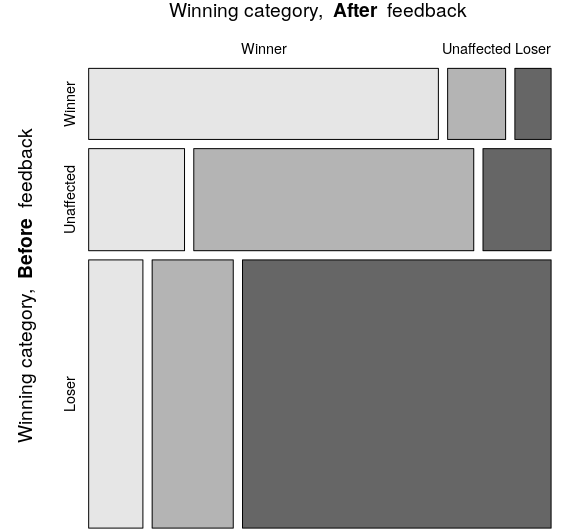
\includegraphics[width=\columnwidth]{Images/transition_matrix_winners.png}
% \caption{Winners (75.8\%)}
% \end{subfigure}\hfill
% \begin{subfigure}{.5\textwidth}
% \centering
% 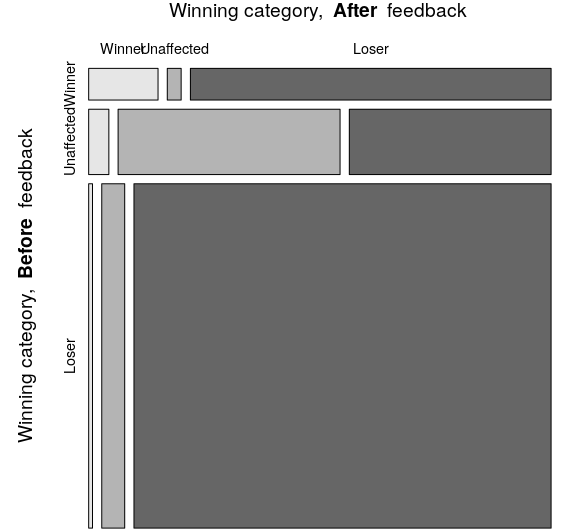
\includegraphics[width=\columnwidth]{Images/transition_matrix_losers.png}
% \caption{Losers (24.2\%)}
% \end{subfigure}
% \caption{Transition matrix among simulated...}
% \label{fig:transition_matrix}
% \end{figure}

%To rigorously show the persistence of pessimistic beliefs, we present in Table \ref{table:confidence_intervals_beliefs_feedback} the share of respondents whose beliefs are aligned with our feedback, and the corresponding 95\% binomial confidence intervals. Given the base rate information provided to respondents that our prediction is correct in five cases out of six, a perfect updating would have yield 83\% of answers aligned with our feedback. This value belongs to the 95\% confidence interval for respondents who receive a ``lose'' feedback ($\widehat{\Gamma} < 0$), but is far beyond for those who received a ``win'' ($\widehat{\Gamma} > 0$). Consistent with our findings on overestimation of policy costs, respondents are again too pessimistic in their beliefs' revision. They tend to agree much more with negative information about the policy outcome than with positive ones.

%A striking comparison is the difference in beliefs revision between those who initially believed they would win and received a ``lose'' feedback ($G > 0$, $\widehat{\Gamma} < 0$) and their opposite ($G < 0$, $\widehat{\Gamma} > 0$). While 82\% of the former changed their mind following the information, only 12\% of the latter did. In other words, a large majority of agents who initially thought they would lose ($G<0$) were not convinced by a contradictory (and positive) information, while those who initially though they would win ($G>0$) largely believed the negative information provided.

%\noindent
%The asymmetry in responses between the two groups of respondents whose initial beliefs were aligned with the feedback ($G=\widehat{\Gamma}$) is also remarkable. While 79\% of those with a ``win'' prior keep the same belief after receiving a ``win'' signal, their negative counterpart are 94\%. In one case, being told that the prior belief has 5 chances over 6 to be correct seems to increase uncertainty so that more than 1 over 6 people change their answer. In the other, being told that with 5 chances over 6 the household will actually lose confirms this initial belief for more than 5 households over 6. A last evidence of the asymmetry in responses comes from the population who initially answered ``unaffected''. When provided the information that they have 5 chances out of 6 to win, only 22\% of them switch to a ``win'' belief ($G^F > 0$ | $G = 0$, $\widehat{\Gamma} > 0$). Conversely, when provided the information that they have 5 chances out of 6 to lose, 45\% switch to this answer ($G^F < 0$ | $G = 0$, $\widehat{\Gamma} < 0$). Overall, it seems therefore that respondents align their beliefs much more when provided negative news about the tax outcome than positive ones.

%they still agree more thantheG= 0type ?

%Considering respondents who receive $\widehat{\Gamma} > 0$, the departure from perfect updating is clear. Even for respondents who initially answered they would win, the probability to keep this belief after a confirming feedback ($G^F > 0$ | $G > 0$, $\widehat{\Gamma} > 0$) has only a 2.5\% probability to be equal to 83.4\% or higher. Although we should expect these individuals to have private information such that they have more than 5 chances over 6 to win, they react to the feedback in the opposite direction.

\paragraph{Determinants of correct updating}


\begin{table}[!htbp] \centering 
  \caption{Asymmetric updating of winning category} 
  \label{asymmetric_simple} 
\makebox[\textwidth][c]{ \begin{tabular}{@{\extracolsep{5pt}}lcccc} 
\\[-1.8ex]\hline 
\hline \\[-1.8ex] 
\\[-1.8ex] & \multicolumn{4}{c}{Correct updating ($U$)} \\ 
\\[-1.8ex] & (1) & (2) & (3) & (4)\\ 
\hline \\[-1.8ex] 
 Constant & 0.120 & $-$0.035 & $-$0.146 & $-$0.116 \\ 
  & (0.012) & (0.179) & (0.178) & (0.179) \\ 
  Winner, before feedback ($\dot{G}$) & 0.695 & 0.685 & 0.646 & 0.659 \\ 
  & (0.078) & (0.080) & (0.080) & (0.080) \\ 
  Initial tax: PNR (I don't know) &  &  & 0.163 & 0.165 \\ 
  &  &  & (0.031) & (0.067) \\ 
  Initial tax: Approves &  &  & 0.158 & $-$0.056 \\ 
  &  &  & (0.046) & (0.115) \\ 
  Diploma (1 to 4) &  & 0.015 & 0.016 & 0.011 \\ 
  &  & (0.013) & (0.013) & (0.014) \\ 
  Diploma $\times$ Initial tax: PNR &  &  &  & $-$0.001 \\ 
  &  &  &  & (0.025) \\ 
  Diploma $\times$ Initial tax: Approves &  &  &  & 0.074 \\ 
  &  &  &  & (0.037) \\ 
  Retired &  & 0.143 & 0.146 & 0.142 \\ 
  &  & (0.080) & (0.079) & (0.079) \\ 
  Active &  & 0.165 & 0.175 & 0.175 \\ 
  &  & (0.055) & (0.054) & (0.054) \\ 
  Student &  & 0.249 & 0.234 & 0.239 \\ 
  &  & (0.076) & (0.075) & (0.075) \\ 
  Yellow Vests: PNR &  & $-$0.048 & $-$0.043 & $-$0.044 \\ 
  &  & (0.047) & (0.047) & (0.047) \\ 
  Yellow Vests: understands &  & $-$0.090 & $-$0.063 & $-$0.064 \\ 
  &  & (0.034) & (0.034) & (0.034) \\ 
  Yellow Vests: supports &  & $-$0.101 & $-$0.059 & $-$0.060 \\ 
  &  & (0.035) & (0.036) & (0.036) \\ 
  Yellow Vests: is part &  & $-$0.172 & $-$0.137 & $-$0.138 \\ 
  &  & (0.062) & (0.062) & (0.062) \\ 
 \hline \\[-1.8ex] 
Among invalidated & \checkmark & \checkmark & \checkmark & \checkmark \\ 
Includes controls &  & \checkmark & \checkmark & \checkmark \\ 
Observations & 1,365 & 1,365 & 1,365 & 1,365 \\ 
R$^{2}$ & 0.055 & 0.111 & 0.133 & 0.136 \\ 
\hline 
\hline \\[-1.8ex] 
\DIFaddbeginFL 

\DIFaddendFL \end{tabular} 
 } \\ \quad \\ {\footnotesize \textsc{Note:} Omitted variables are \textit{Unemployed/Inactive} and \textit{Yellow Vests: opposes}. The list of controls can be found in Appendix \ref{set_controls}. }  \end{table}  
% \begin{table}[!htbp] \centering 
%   \caption{Asymmetric updating of winning category} 
%   \label{asymmetric_simple} 
% \makebox[\textwidth][c]{ \begin{tabular}{@{\extracolsep{5pt}}lccc} 
% \\[-1.8ex]\hline 
% \hline \\[-1.8ex] 
% \\[-1.8ex] & \multicolumn{3}{c}{Correct updating ($U$)} \\ 
% \\[-1.8ex] & (1) & (2) & (3)\\ 
% \hline \\[-1.8ex] 
%  Constant & 0.120 & $-$0.041 & $-$0.150 \\ 
%   & (0.012) & (0.190) & (0.189) \\ 
%   Winner, before feedback ($\dot{G}$) & 0.695 & 0.685 & 0.646 \\ 
%   & (0.078) & (0.080) & (0.080) \\ 
%   Initial tax: PNR (I don't know) &  &  & 0.163 \\ 
%   &  &  & (0.031) \\ 
%   Initial tax: Approves &  &  & 0.158 \\ 
%   &  &  & (0.046) \\ 
%   Retired &  & 0.143 & 0.146 \\ 
%   &  & (0.080) & (0.079) \\ 
%   Active &  & 0.165 & 0.175 \\ 
%   &  & (0.055) & (0.054) \\ 
%   Student &  & 0.249 & 0.234 \\ 
%   &  & (0.076) & (0.075) \\ 
%   Yellow Vests: PNR &  & $-$0.048 & $-$0.043 \\ 
%   &  & (0.047) & (0.047) \\ 
%   Yellow Vests: understands &  & $-$0.090 & $-$0.063 \\ 
%   &  & (0.034) & (0.034) \\ 
%   Yellow Vests: supports &  & $-$0.101 & $-$0.059 \\ 
%   &  & (0.035) & (0.036) \\ 
%   Yellow Vests: is part of &  & $-$0.172 & $-$0.137 \\ 
%   &  & (0.062) & (0.062) \\ 
%  \hline \\[-1.8ex] 
% Among \textit{invalidated} & \checkmark & \checkmark & \checkmark \\ 
% Controls: Socio-demo, politics, estimated gains &  & \checkmark & \checkmark \\ 
% Observations & 1,365 & 1,365 & 1,365 \\ 
% R$^{2}$ & 0.055 & 0.111 & 0.133 \\ 
% \hline 
% \hline \\[-1.8ex] 
%DIF <  & \multicolumn{3}{r}{p$<$0.1; p$<$0.05; p$<$0.01} \\ 
%DIF >  
% \end{tabular} 
%  } \\ \quad \\ {\footnotesize \textsc{Note:} Omitted variables are \textit{Unemployed/Inactive} and \textit{Yellow Vests: opposes}. The list of controls can be found in Appendix \ref{set_controls}. }  \end{table}  

The observed asymmetry in beliefs' revision echoes a recent literature that has emphasized how people selectively process information regarding themselves or specific events, generally in \DIFdelbegin \DIFdel{an over-optimistic way \mbox{%DIFAUXCMD
\citep[][]{eil_good_2011,mobius_et_al_2011,sharot_et_al_2011}}\hspace{0pt}%DIFAUXCMD
. By contrast, our }\DIFdelend \DIFaddbegin \DIFadd{a way that satisfies their ego \mbox{%DIFAUXCMD
\citep[][]{eil_good_2011,mobius_et_al_2011,sharot_et_al_2011}}\hspace{0pt}%DIFAUXCMD
. Our }\DIFaddend results show that in the case of a policy considered as undesirable, people give more weight to negative news. \DIFdelbegin \DIFdel{Still}\DIFdelend \DIFaddbegin \DIFadd{Thus}\DIFaddend , both results are consistent with individuals forming their beliefs in a motivated way. To assess the extent of motivated reasoning, we analyze the heterogeneity in people's updating. To handle the notion of \textit{correct updating}, we define a variable $U$ which equals $+1$ if the respondent adopts a feedback that invalidates their initial belief, $-1$ if they update against the feedback that confirms it, or $0$ if they do not update. Over the sub-sample of \textit{invalidated} respondents who should have updated because their initial winning category is not aligned with our feedback, we regress the \textit{correct updating}, $U$, over the initial belief not to lose, $G^I$, and a vector of characteristics, \textbf{C}:
% diagram flow among those who should have updated upwards -> càd ? on oublie

\begin{equation}
	U_{i} = \delta_{0}+\beta_{U}G^I_{i}+\mathbf{\beta_C C}+\epsilon_{i}\hspace{0.3cm} \text{for}\,i:\,\text{sgn}\left(g_i\right)\neq\text{sgn}\left(\hat{\gamma}_i\right),
\end{equation}

\noindent
where $\text{sgn}$ is the sign function. The high value for $\beta_{U}$ reported in column (1) of Table \ref{asymmetric_simple} again proves that, among those who should have updated, those who initially think they would win (the optimistic losers) update significantly more correctly than those who do not think so (the pessimistic winners). Many other specifications have been tested, depending on how the unaffected are treated and whether controls are included or not, or with the winning category after the feedback as covariate, and they all confirm a win/lose asymmetry in updating.

% with the winning category after the feedback as covariate, and 
%Reciprocally, we can regress $U$ on the winning category after the feedback, over the same sub-sample of respondents who should have updated:
%\begin{equation}
%	U_{i}=\delta_{0}+\beta^{\prime}_{U}G_{i}^{F}+\epsilon_{i}\,|\,\dot{G_{i}} = %-\widehat{\Gamma_{i}}
%\end{equation}
%\noindent
%Again, $\beta^{\prime}_{U}$ is significantly above $0$ (see column (3) of Table \ref{asymmetric_simple}), suggesting a bias towards loss when updating. Indeed, among those who should have updated, those who end up as winner are disproportionately more correct in thinking so than those who switch or stay as losers.


Beyond this asymmetry, column (2) shows that some respondents' characteristics are correlated with correct updating. Relative to unemployed and inactive people, retired, active, and students update more correctly, the latter being 25 p.p. more likely to correctly revise their beliefs when invalidated than unemployed and inactive. Similarly to perceptions of net gains, position towards the Yellow Vests is significantly correlated with correct updating. The magnitude of this effect is large, as people who are part of the movement are 17 p.p. less likely to correctly update than people who oppose it. This can be linked to the Yellow Vests' higher distrust of the government, documented in \citet{algan_et_al_19}, that could apply to information provided by researchers regarding policies. Column (3) includes disapproval as a covariate: it indicates that, as for the initial bias in subjective gains, disapproving the reform is associated with a less correct update by 16 p.p. and partly explains the effect of the Yellow Vests. Appendix \ref{app:mr} confirms that the result holds true when \DIFaddbegin \DIFadd{initial }\DIFaddend subjective gains are accounted for, ruling out the explanation that this less correct updating is entirely due to specific priors of those who disapprove the reform. 

\paragraph{Motivated reasoning} % Explanatory mechanisms

%Druckman & McGrath 2019 NCC propose MR to explain CC beliefs polarization, but say lack of evidence (formal model from Little, and Kraft et al for detailed mechanisms, Le Yaouanq endogeneizes motivations through self-interest); evidence for model in other context: Redlawsk) + Kahan: characterizes MR on CC as rational

The previous result suggests that conservatism in belief revision does not simply follow from people's cognitive difficulties when dealing with Bayes' rule. The higher likelihood to update correctly of those who approve the reform is robust evidence that ideology and political identity shape belief formation. Such directional motivated reasoning has been proposed by \citet{druckman_evidence_2019} to explain polarization around beliefs on climate change. \citet{kahan_ideology_2013} provides empirical evidence that political motivated reasoning about climate change is not a reasoning deficiency but rather a reasoning adaptation following the interest that individuals have in conveying ``their membership in and loyalty to affinity groups central to their personal well-being''. In our case, the position relative to the Yellow Vests proxies the groups that respondents identify with, and the differentiated updating along this spectrum can be interpreted as motivated reasoning. Besides, the hypothesis that motivated reasoning follows from a rational adaptation purpose implies that better educated people are \textit{more} prone to motivated reasoning, as they are more able to formulate specious reasonings and reconcile antagonistic information and ideas. Column (4) supports this hypothesis, as the interaction term between diploma and initial tax approval is positive and significant, even capturing all the effect of initial tax approval. To our knowledge, this result is the first robust evidence of directional and rational motivated reasoning in the context of climate policies, and it provides empirical support for various models of endogenous belief formation. For example, \citet{little_distortion_2019} formalizes the idea that directional motives may override accuracy motives and update auxiliary beliefs (in our case, the winning category) in order to preserve their consistency with core beliefs (here, rejection of the tax). Building upon the cognitive and social mechanisms described by \citet{kraft_why_2015} and documented by e.g. \citet{redlawsk_hot_2002}, we hypothesize the following narrative as one of the possible channels through which aversion for the carbon tax became entrenched. The Yellow Vests first gathered to defend their interest (above all their purchasing power), and a side effect of the daily interactions on roundabouts was to bring material and emotional support to the protesters \citep{challier_rencontres_2019}. A group identity soon developed, which crystallized shared beliefs and affects such as a rejection of carbon taxation. This group identity gained support from a large majority of the population, notably through social networks. Now, due to the loyalty to the group as well as the affects that have entered their subconscious, Yellow Vests supporters oppose instinctively any carbon tax, and are prone to find excuses to cope with contradictory messages, e.g. by denying the reliability of these messages \citep{golman_preference_2016}. Admittedly, such a narrative falls short of explaining the majority rejection among those who oppose the Yellow Vests (which may originate from biased perceptions more than tax aversion), but it illustrates how biased beliefs can be so persistent among Yellow Vests supporters.
% Suggestion: To conclude, self-interest, affects, and trust in the government and in sources of information all influence beliefs and preferences, and the present paper is just a first step to disentangle all these effects.
%DIF <  DONE: nouvelles références: Challier; Golman et al. Le second c'est un papier d'éco sur comment on recherche à avoir des croyances cohérentes avec celles d'un groupe, pas sûr qu'lle soit bien introduite. La 1ere c'est de la socio et ça permet ptet de retirer la footnote. -> Done : footnote retirée : "\footnote{See also Florence Aubenas' \href{https://www.lemonde.fr/societe/article/2018/12/15/sur-les-ronds-points-les-gilets-jaunes-a-la-croisee-des-chemins_5397928_3224.html}{investigation} for \textit{Le Monde}.}"
%DIF >  DONE: nouvelles références: Challier; Golman et al. Le second c'est un papier d'éco sur comment on recherche à avoir des croyances cohérentes avec celles d'un groupe, pas sûr qu'lle soit bien introduite. La 1ere c'est de la socio et ça permet ptet de retirer la footnote. \footnote{See also Florence Aubenas' \href{https://www.lemonde.fr/societe/article/2018/12/15/sur-les-ronds-points-les-gilets-jaunes-a-la-croisee-des-chemins_5397928_3224.html}{investigation} for \textit{Le Monde}.}

%In particular, \citet{little_distortion_2019} formalizes some of the cognitive and social mechanisms detailed by \citet{kraft_why_2015}, while \citet{le_yaouanq_model_nodate} endogeneizes the directional motive as stemming from self-interest.  
% les gilets jaunes se sont constitués pour défendre leur intérêt, ça a entraîné une identité propre qui a procuré du soutien émotionnel et matériel à ses membres, de même que ça a développé des affects négatifs à l'égard de la taxe carbone, alors maintenant tant par loyauté au groupe auquel ils s'identifient que par préjugés, ils s'opposent intuitivement à toute taxe carbone, car la recherche de cohérence avec les idées de leur groupe l'emporte sur la recherche d'exactitude. Ceux qui sont les plus à même de former des raisonnements spécieux qui mettent en cohérence les informations contradictoires avec leur intention initiale sont les plus éduqués, d'où l'effet observé.
%ça peut avoir l'air tiré par les cheveux de prime abord mais j'invente rien, Kahan 2013, Kraft 2015 et Redawsk 2016 par ex, montrent ces effets
%et de conclure : l'intérêt personnel, les affects et la confiance envers le gouvernement se mêlent pour former les croyances et les préférences, et des recherches ultérieures permettraient de démêler les trois

% old: The previous results suggest that conservatism in belief revision does not simply follow from people's cognitive difficulties when dealing with Bayes' rule. The determinants identified (``win'' vs. ``lose'' feedback, attitude towards the policy, and the Yellow Vests) rather indicate that belief formation and revision are intrinsically linked to preferences, a mechanism known as ``motivated reasoning'' in the literature \citep{ziva_kunda_case_1990}. Closely related is the well documented ``confirmation bias'', the tendency to weigh information differently depending on whether it confirms a prior belief or not. More recently, studies have also shown evidence of a ``good news -- bad news effect'' \citep{eil_good_2011,sharot_et_al_2011}, meaning that people tend to give more weight to information that satisfies their ego or self-interest. Our results go \textit{a priori} in the opposite direction, since people discard what we could consider ``positive'' news $(\widehat{\Gamma} = 1)$ but not negative ones $(\widehat{\Gamma} = 0)$. Still, this effect is consistent with motivated reasoning as the lack of update has been shown much stronger for people who disapprove of the policy and for supporters of the Yellow Vests. Thus, people's positioning does not only bias their initial perception about the policy, but also how they process new information about it. % *** dans cette phrase, j'ai l'impression que ce n'est pas clair si on remplace "positioning" par "position". => !! ok

% A second explanation for the difficulty to convince some people is their distrust towards third parties, such as the State or media, that could apply to information provided by researchers. As shown by (ref), supporters of Yellow Vests trust the State less than supporters of any political party. A recent Avaaz report also documented the high receptivity of Yellow Vests followers to fake news on social media.

% The determinants identified (``win'' vs. ``lose'' feedback, attitude towards the policy and the Yellow Vests) rather indicate that beliefs formation and revision are intrinsically linked to trust and preferences. As shown by (ref), on average supporters of Yellow Vests trust the State less than supporters of any political parties including extreme right. A recent Avaaz report also documented the high receptivity of Yellow Vests followers to fake news on social media. The lack of trust in third parties could also apply to information provided by researchers.

%a mechanism known as ``motivated reasoning'' in the literature \citep{ziva_kunda_case_1990}.

    \subsection{Environmental effectiveness}\label{subsec:update_ee}


Table \ref{tab:update_ee} in Appendix \ref{subsec:app_perception_ee} reports the effect of displaying relevant information on the belief that our Tax \& Dividend is environmentally effective. The effect of reporting a scientific consensus on environmental effectiveness ($E$) is positive and statistically significant, but its magnitude --- around 5 p.p. --- seems modest given that the question immediately follows the priming. The effects of information on climate change ($CC$) or particulates ($PM$) are smaller, and only $CC$ is significant, which is understandable as they were displayed at the very beginning of the survey and do not mention any environmental policy. As suggested by \citet{millner_beliefs_2016}, given the complexity of the mechanisms at play, drawing a causal link between causes and consequences of environmental problems requires considerable cognitive effort, making it difficult to convince one about the effectiveness of policies that decentralize efforts to tackle pollution. Finally, we observe that our primings have no significant effect on beliefs over causes and consequences of climate change. Overall, these primings appear insufficient to change most people's mind about climate change and carbon tax effectiveness. % suggestion: ajouter une phrase pour dire que ça reste une question ouverte à quel point on pourrait convaincre les gens avec des arguments plus détaillés ?

%Table \ref{first_stage_environmental_effectiveness} in Appendix \ref{subsec:app_motives_1st_stage} reports the effect of displaying relevant information on the belief that Tax \& Dividend is environmentally effective. Each priming is associated with a lower propensity to believe the scheme is ineffective by 4 p.p. The effect of reporting a scientific consensus on environmental effectiveness ($E$) is significant, but its magnitude seems quite low, given that the question immediately follows the priming. Even with the same magnitude, effects of information on climate change ($CC$) or particulates ($PM$) seem more important, as these primings were displayed at the very beginning of the survey, and as they do not mention any environmental policy. As suggested by \citet{millner_beliefs_2016}, given the complexity of the mechanisms at play, making a causal link between causes and consequences of environmental problems requires considerable cognitive efforts. It is thus remarkable that the effect of these primings is comparable to our more direct information on the policy's effectiveness. Besides, it is worth noticing that receiving both pieces of information has the same effect as receiving only one of them. Finally, we observe that our primings have no significant effect on beliefs over causes and consequences of climate change. Overall, these primings appear insufficient to change most people's mind about climate change and carbon tax effectiveness.
% , but slightly changes the perceptions of which generations will be affected


   \subsection{Progressivity\label{subsec:persistence-prog}}

Table \ref{tab:prog} in Appendix \ref{subsec:app-prog} shows the absence of effect of explaining that our Tax \& Dividend is progressive on perceived progressivity: the correlation between the two is close to 0 (at $-0.006$) and even has an unexpected negative sign. Column (2) of the same table clarifies why our treatment does not change the overall share of people who think the policy is regressive: those who have a large bias in their perception of gains are in fact \textit{more} prone to perceive \textit{regressivity} once provided the information, by 13 p.p. This result may be a manifestation of the boomerang effect with people inclined to motivated reasoning, which has already been documented for Republican attitudes over climate change in the \DIFdelbegin \DIFdel{U.S. }\DIFdelend \DIFaddbegin \DIFadd{US }\DIFaddend \citep{zhou_boomerangs_2016}. Indeed, \citet{hovland_communication_1953} showed that when someone is pressured to make a certain choice, psychological reactance \citep[theorized by][]{brehm_theory_1966} can cause them to resist this pressure by adopting an opposite alternative.  Although the effect on those without a large bias is not significant, providing them with information is associated with a lower perceived regressivity by 5 p.p. A possible explanation for the strong belief in regressivity is that people view the tax as regressive (relative to income) and the transfer as neutral (in absolute values), and mistakenly conclude that their combination is regressive. In any case, without a deep explanation of the underlying mechanisms, the progressivity of the policy remains unintuitive for most people, and we cannot convince them easily.

%Somewhat surprisingly, there is not significant interaction between perceived progressivity and income on the winning category. => plutôt dans l'autre papier, ou dans section 3.

% Do regressions to see the effect of information on different outcomes => results hard to interpret 
% effect on gain depending on income => no clear effect
% Discuss link with political positionning => no clear effect
% Assess to what extent are these people different than others, using several socio-demo that we could regress on updating. => somehow done in table 'Determinants of bias in subjective gains'



\section{\DIFdelbegin \DIFdel{Motives for acceptance }\DIFdelend \DIFaddbegin \DIFadd{How beliefs determine attitudes }\DIFaddend \label{sec:motives5}}

Our results clearly indicate that, as of today, a carbon tax is unlikely to be accepted in France. However, we have also shown that people largely display incorrect perceptions about the true effects of the policy. Most of them overestimate the negative impact on their purchasing power, think that the policy is regressive, and do not see it as environmentally effective. In this section, we examine to what extent the low acceptance rate reflects intrinsic preferences or wrong perceptions. The question we address is whether correcting biased beliefs would be sufficient for a carbon tax to be accepted. 

    \subsection{Self-interest}

\paragraph{Identification challenge}

\DIFdelbegin \DIFdel{While }\DIFdelend %DIF >  Suggestion: parmi les gens se pensant initialement perdants mais qu'on convainc qu'ils sont non perdants, l'acceptation augmente de 30%: c'est l'effet de passer de "croire vaguement en la perte" à "se savoir gagnant". Ce qu'on mesure avec l'IV c'est l'effet de "se savoir gagnant" par opposition à "se savoir perdant" (cf. analyse.R fin de 5.1, où il y a d'autres stats).  je mets un to do juste pour que tu voies cette suggestion, même si tu y avais déjà pensé, et même si on ne va pas le rajouter pour AER pck il ne faut pas rallonger -> Ok
%DIF >  DONEw: replace "While three-quarters of the respondents are expected to win from our Tax \& Dividend, 62\% of these winners consider that they would not win and disapprove of the policy." by "Among the three-quarters of the respondents expected to win from our Tax \& Dividend, 62\% both consider that they would not win and disapprove of the policy."
\DIFaddbegin \DIFadd{Among the }\DIFaddend three-quarters of the respondents \DIFdelbegin \DIFdel{are }\DIFdelend expected to win from our Tax \& Dividend, 62\% \DIFdelbegin \DIFdel{of these winners }\DIFdelend \DIFaddbegin \DIFadd{both }\DIFaddend consider that they would not win and disapprove of the policy. We want to estimate to what extent knowing they would win would lead them to approve of the reform. Because respondents thinking they would win might differ in many respects from those thinking they would not, we cannot simply regress approval on perception of winning. 

%For instance, one could imagine that a person thinking she might lose would also be more likely to think that most people would lose, and thus be more likely to disapprove.

\paragraph{Main identification strategy}

% T & td -> a T & TD; affected -> assigned; Let us -> We; eligible to -> for; approves OF; two stage least-square model -> two-stage least square model
In order to identify the effect \textit{ceteris paribus} of self-interest on acceptance, we exploit exogenous variations in gains and losses. To do so, we consider a Tax \& Targeted Dividend, where respondents are randomly assigned to a compensation scheme to which they are eligible or not (see section \ref{subsubsec:the-survey}). Our methodology mixes a random discontinuity design (RDD) and an instrumental variable (IV) strategy. We denote by $I_{1,i}$ respondent's $i$ income, and by $I_{2,i}$ the income of the second adult of their household if there is one, which we control for with a dummy variable $S_i$ equal to 1 when there is a single adult. Let $T_{1,i}$ and $T_{2,i}$ be two binary variables indicating whether these individuals would be eligible for the transfer.\footnote{As explained in section \ref{subsubsec:the-survey}, we explicitly limit the number of beneficiaries to two per household.} We also denote by $G_i^T$ a dummy variable equal to 0 if respondent $i$ thinks they would lose from the Tax \& Targeted Dividend, and 1 otherwise. Similarly, $A_i^T$ is a dummy variable equal to 0 if respondent $i$ disapproves of this policy and 1 otherwise. We can then write a two-stage least square model, with the following first stage equation:
% Suggestion: si AER, citer Lemieux (RDD). -> utile pour montrer qu'on connait l'existence de ce papier et qu'on sait ce qu'on fait avec la RDD.

%  include figure below: -> je ne suis pas sûr que ce soit pertinent, on a déjà les first stage te 2nd stage. Ca nous obligerait à discuter cette figure et expliquer davantage pourquoi tout le monde ne se croit pas gagnant lorsqu'ils sont eligibles.

% \begin{figure}[!htbp]
% \centering
% 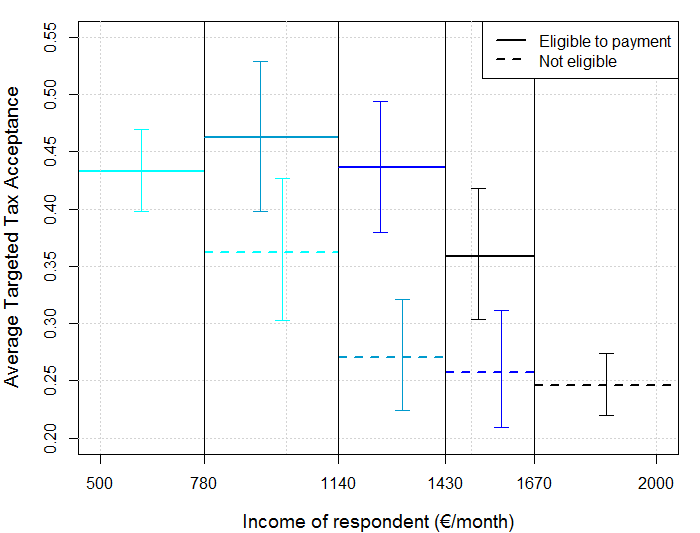
\includegraphics[width=0.75\columnwidth]{Images/RDD_Acceptance_flat_90CI_black.png}
% \caption{Average targeted tax acceptance rate by income category depending on eligibility, with 90\% confidence intervals.}
% \label{fig:rdd-iv}
% \end{figure}

\begin{equation}
%    G_i^T = \alpha_0 + \alpha_1 T_{1,i} + \alpha_2 T_{2,i} + \sum_{j=1}^J \alpha_{j+2} (I_{1,i})^{j} + \sum_{j=1}^J \alpha_{j+2+J} (I_{2,i})^{j} + \eta_i
    G_i^T = \alpha_0 + \alpha_1 T_{1,i} + \alpha_2 T_{2,i} + \alpha_c c_i  + \alpha_S S_i + \sum_{j=1}^2 \left( \alpha_{1,j} I_{1,i}^j + \alpha_{2,j} I_{2,i}^j \right) + \eta_i
    \label{eq:first_stage_parametric_rdd_approve_winner}
\end{equation}

\noindent
where second order terms for income bring more flexibility. We precise that eligibility is defined using income thresholds $c_i$ that are randomly allocated to households (see section \ref{subsubsec:the-survey}) and introduced as fixed effects to control for threshold-specific preferences. Formally, we define eligibility of adult $k\in \{1;2\}$ as:

\begin{equation}
T_{k,i} =
\begin{cases}
  0, & \text{if}\ I_{k,i} > c_i \\
  1, & \text{otherwise}
\end{cases}
\end{equation}

\medskip

\noindent
Finally, the second stage writes:

\begin{equation}
%    A_i^T = \beta_0 + \beta_1 \widehat{G}_i^T + \sum_{j=1}^J \beta_{j+2} (I_{1,i})^{j} + \sum_{j=1}^J \beta_{j+2+J} (I_{2,i})^{j} + \epsilon_i
    A_i^T = \beta_0 + \beta_1 \widehat{G}_i^T + \beta_c c_i + \beta_S S_i + \sum_{j=1}^2 \left( \beta_{1,j} I_{1,i}^j + \beta_{2,j} I_{2,i}^j \right) + \epsilon_i
    \label{eq:second_stage_with_rdd_approve_winner}
\end{equation}

\medskip

\noindent
where $\widehat{G_i}^T$ denotes the fitted value of $G_i^T$ from the first stage regression. As can be seen from first stage results in Appendix \ref{subsec:app_motives_1st_stage}, eligibility of both respondents and households' second adults are positively correlated with beliefs of winning, so both instruments are relevant. The exclusion restriction states that conditional on income, being eligible affects approval solely through beliefs of winning. The RDD procedure employed in the first stage ensures that this is the case: conditional on income, eligibility is random, and controlling for the target, it should affect acceptance only through self-interest.
% Note!: being eligible may not lead to think you win or not because you may anticipate a changing situation (ex: higher income next year so that if you are close to the threshold you lose eligibility).

\paragraph{Alternative specifications for robustness}

To further ensure the robustness of the results, we estimate several alternative specifications. First, we run the same RDD + IV design adding control variables (specification 2). In particular, we control for initial acceptance of our Tax \& Dividend as this should explain most of the variation in the dependent variable. Second, we compare our results with a simple OLS where we control for relevant variables (3). Third, we use a logit model (4) to ensure that imposing linearity does not bias the results. Finally, we exploit a methodology similar to the main specification but applied to the \DIFaddbegin \DIFadd{customized }\DIFaddend feedback, without (5) and with (6) control variables. Indeed, as our estimation of gains for this feedback is a continuous variable $\widehat{\gamma}$, but the feedback itself is a binary variable $\widehat{\Gamma}$, we run an RDD to predict the belief of winning after feedback $G^F$. We then exploit variations around the threshold of zero net gain (which are random conditional on net gain) to explain acceptance $A^F$. This alternative two-stage least square writes: %DIF >  Doneww: add "customized" before feedback

\begin{equation}
    G_i^F = \alpha_0 + \alpha_1 \widehat{\Gamma}_{i} + \sum_{j=1}^2 \alpha_{1,j} (\widehat{\gamma}_{i})^{j} + \eta_i
    \label{eq:first_stage_parametric_rdd_approve_winner_feedback}
\end{equation}

\vspace{-.0cm}

\begin{equation}
    A_i^F = \beta_0 + \beta_1 \widehat{G}_i^F + \sum_{j=1}^2 \beta_{1,j} (\widehat{\gamma}_{i})^{j} + \epsilon_i
    \label{eq:second_stage_feed_with_rdd_approve_winner}
\end{equation}

\vspace{.5cm}

\noindent
where $\widehat{G}_i^F$ denotes the fitted value of $G_i^F$ from the first stage regression. The identification assumption of this second IV states that conditional on estimated net gains $(\widehat{\gamma})$, receiving a win feedback $(\widehat{\Gamma} = 1)$ affects approval solely through self-interest. Finally, we also investigate alternative versions of the previous models where we estimate the effect to ``win'' instead of ``not to lose'', and on ``approval'' instead of ``acceptance''.

\paragraph{Results}


\begin{table}[!htbp] \centering 
  \caption{Effect of self-interest on acceptance.} 
  \label{results_private_benefits} 
\makebox[\textwidth][c]{ \begin{tabular}{@{\extracolsep{5pt}}lcccccc} 
\\[-1.8ex]\hline 
\hline \\[-1.8ex] 
\\[-1.8ex] & \multicolumn{4}{c}{Targeted Acceptance ($A^T$)} & \multicolumn{2}{c}{Feedback Acceptance ($A^F$)} \\ 
\\[-1.8ex] & \multicolumn{2}{c}{\textit{IV}} & \textit{OLS} & \textit{logit} & \multicolumn{2}{c}{\textit{IV}} \\ 
\\[-1.8ex] & (1) & (2) & (3) & (4) & (5) & (6)\\ 
\hline \\[-1.8ex] 
 Believes does not lose & 0.571 & 0.567 & 0.443 & 0.431 & 0.517 & 0.434 \\ 
  & (0.092) & (0.092) & (0.014) & (0.018) & (0.170) & (0.135) \\ 
  Initial tax Acceptance ($A^I$) &  & 0.339 & 0.360 & 0.342 &  & 0.428 \\ 
  &  & (0.033) & (0.026) & (0.034) &  & (0.055) \\ 
 \hline \\[-1.8ex] 
Controls: Incomes  & \checkmark  & \checkmark  & \checkmark   & \checkmark  &   & \checkmark \\ 
Controls: Estimated gain  &  & \checkmark  & \checkmark  & \checkmark  & \checkmark & \checkmark \\ 
Controls: Target of the tax  & \checkmark  & \checkmark  & \checkmark  & \checkmark   &  &  \\ 
Controls: Socio-demo, other motives  &  & \checkmark  & \checkmark  & \checkmark   &  & \checkmark   \\ 
Observations & 3,002 & 3,002 & 3,002 & 3,002 & 1,968 & 1,968 \\ 
R$^{2}$ & 0.033 & 0.302 & 0.470 &  & 0.044 & 0.526 \\ 
\hline 
\hline \\[-1.8ex] 
  \DIFaddbeginFL 

\DIFaddendFL \end{tabular} 
} {\footnotesize \\ \quad \\ \textsc{Note:} Standard errors are reported in parentheses. For logit, average marginal effects are reported and not coefficients. The list of controls can be found in Appendix \ref{set_controls}. }\end{table} 

% DONE: powerful -> highly efficient (strong?) => *** Problème : tous ces termes ont un sens assez spécifique en économétrie. Je pense qu'efficient est à éviter pour cette raison. Strong peut aussi induire en erreur avec l'IV. J'ai remis powerful qui me semble le plus adapté parce que cela renvoie à "explanatory power", ce qui est pertinent pour une variable de contrôle et en particulier celle-ci. => !! oui tu as raison, Christina ne connaît pas les termes d'économétrie c'est pour ça que ça lui a paru bizarre
% and the difference due -> and that the difference is due; remove a coma; add one after 6; 
First stage regression results are given in Appendix \ref{subsec:app_motives_1st_stage}. The effective F-Statistics \citep{montiel_pflueger_2013} range from 37 to 57, indicating that both targeted transfers and feedback are strong instruments. Table \ref{results_private_benefits} provides the second stage results for the six main specifications, and additional specifications can be found in Appendix \ref{subsec:app_motives_other}. Overall, the estimated effects of self-interest indicate that believing not to lose increases acceptance by about 50 p.p. The results obtained for the local average treatment effect (LATE) on compliers in IV regressions --- i.e. on people who recognize they would not lose because of the treatment --- are significantly higher than for the average treatment effect (ATE) estimated with OLS (57 vs. 44 p.p. for Tax \& Targeted Dividend). Given the wide set of control variables used, and in particular our powerful control $A^I$, one can be rather confident that the OLS estimate is unbiased, and that the difference is due to the specificity of compliers in the LATE. This explanation holds for both the targeted scheme and acceptance after feedback and is supported by the findings of section \ref{subsec:update_si} for the latter. Indeed, as respondents most likely to revise their beliefs after a ``win'' feedback are also more in favor of the tax, the IV coefficient for compliers is logically higher than the point estimate found with OLS. The comparisons of columns 1 with 2, and 5 with 6, show that adding control variables does not significantly affect the coefficient for Tax \& Targeted Dividend, but does for acceptance after feedback, where the controls seem to capture part of the specificity of compliers. Overall, both methods yield similar effects: 57 p.p. with targeted transfers and 52 p.p. with the feedback. Finally, results from the logit regression (4) confirm that the assumptions of the linear probability model (LPM) do not bias the results.\footnote{Separation occurs in logistic regressions for self-interest and effectiveness. We made sure this does not lead to biased coefficients by conducting likelihood ratio tests and by running penalized regressions \citep{firth_bias_1993,heinze_fixing_2003}. }
% With Firth regressions, coefficients change by no more than 3\%.
% The self-interest coefficient is also larger for targeted transfers (57 p.p.) than after feedback (52 p.p.), though not significantly. This may come from the higher average gains of winners for targeted mechanisms and stress that beyond a binary view of ``win''/``lose'', the magnitude of gains matter for acceptance. 
% As we have shown in section \ref{subsec:update_si}, one can identify based on observable characteristics the respondents most likely to revise their beliefs after a ``win'' feedback. As respondents less likely to update are also initially less in favor of the tax, the difference between these sub-populations may explain the lower point estimate found with OLS for the feedback. ... As shown in section \ref{subsec:update_si}, the respondents most likely to trust our feedback differ from the average, hence adding controls (and in particular on other acceptance motives) likely captures part of the specificity of compliers. 


By isolating \textit{beliefs} about self-interest \textit{ceteris paribus}, we showed that this motive has a large effect on carbon tax acceptance. This result confirms previous findings of the literature  \citep{stern_value_1993,thalmann_public_2004,baranzini_effectiveness_2017}, but contrasts with the results of \citet{kallbekken_saelen_2011} who found that self-interest plays a limited role in Norway. Their different result could come from their methodological approach that relies on proxies to capture self-interest in regressions, or on differences between preferences of French and Norwegian people. Our results also qualify the findings of \citet{anderson_can_2019} who suggest that ideology better predicts carbon tax acceptance than self-interest. By distinguishing beliefs from preferences, we find that ideology plays an indirect role by shaping beliefs about one's self-interest, and that beliefs directly affect acceptance.

%come from differences between preferences of French and Norwegian people, or from their methodological approach that relies on proxies to capture self-interest in regressions. Indeed, \citet{anderson_can_2019} shows that ideology and beliefs better predict carbon tax acceptance than objective gains, which suggests that beliefs of self-interest are poorly proxied by objective gains.

    \subsection{Environmental effectiveness}\label{subsec:motive_ee}

% Note!: Interprétation du LATE. Imbens : "Without (...) assumptions we can only identify average effects for subpopulations that are induced by the instrument to change the value of the endogenous regressors". Maybe those who change their mind because of information on CC (i.e. compliers) are much more receptive than others..

\paragraph{Main identification strategy}

One of the strongest barriers to carbon tax implementation is a widespread perception of its environmental ineffectiveness. Our objective is therefore to assess to what extent learning about the environmental benefits of the tax could increase acceptance. To identify this effect, we estimate a two-stage least squares (2SLS) where the first stage uses random information to explain beliefs about environmental effectiveness, while the second stage regresses acceptance on the fitted exogenous variations in these beliefs. Because information on particulate matter ($Z_{PM}$) is poorly correlated with beliefs of effectiveness, we restrict the set of instruments to our primings on the scientific consensus ($Z_{E}$) and climate change ($Z_{CC}$). As discussed in section \ref{subsec:update_ee}, these instruments are significantly related to our endogenous variable, yet are potentially weak, as our primings do not have a large effect on people's beliefs. If we denote by $E$ a dummy variable equal to 0 if the respondents think the policy is not environmentally effective and 1 otherwise, we can write a 2SLS model as follows:

\begin{equation}
    E_i = \alpha_0 + \alpha_1 Z_{E,i} + \alpha_2 Z_{CC,i} + \mathbf{\alpha_C C_i}  + \eta_i
    \label{eq:first_stage_parametric_rdd_approve_effective}
\end{equation}
%+ \mathbf{\alpha} \cdot \mathbf{C_i}  + \mathbf{\beta} \cdot \mathbf{C_i}

\vspace{-.5cm}

\begin{equation}
    A^I_i = \beta_0 + \beta_1 \widehat{E}_i + \mathbf{\beta_C C_i} + \epsilon_i
    \label{eq:second_stage_parametric_rdd_approve_effective}
\end{equation}

\vspace{.5cm}

\noindent
where $\widehat{E}_i$ denotes the fitted value of $E_i$ from the first stage regression, and $\textbf{C}$ a vector of characteristics.

\paragraph{Alternative specifications for robustness checks}

To ensure the robustness of our results, we estimate the previous 2SLS with control variables (1). Acknowledging that our primings could affect acceptation motives other than effectiveness alone, this potential bias should disappear when controlling for many variables including other motives. In addition, we estimate an OLS (2) model to compare the LATE of the first specifications with an ATE, and a logit model (3) to check the robustness of assumptions underlying the linear probability model. Finally, we also estimate two modified versions of our main specifications, where we switch from broad to strict definitions for environmental effectiveness (4) and for tax approval (5).
% We do not control for progressivity: as most of the people who did not answer the question were in the second half of the survey, the absence of response is too correlated with our instrument Z_EE (apres_modifs) which bias the results.

%As information provided in our primings could potentially affect respondents' preferences by other mechanisms than through beliefs about tax' environmental effectiveness, 

\paragraph{Results}

\begin{table}[!htbp] \centering 
  \caption{Effect of believing in environmental effectiveness on acceptance} 
  \label{tab:ee} 
\makebox[\textwidth][c]{ \begin{tabular}{@{\extracolsep{5pt}}lccccc} 
\\[-1.8ex]\hline 
\hline \\[-1.8ex] 
\\[-1.8ex] & \multicolumn{4}{c}{Tax Acceptance ($A^I$)} & Tax Approval ($\dot{A^I}$) \\ 
\\[-1.8ex] & \textit{IV} & \textit{OLS} & \textit{logit} & \textit{IV} & \textit{IV} \\ 
\\[-1.8ex] & (1) & (2) & (3) & (4) & (5)\\ 
\hline \\[-1.8ex] 
 Environmental effectiveness: not ``No'' & 0.479 & 0.391 & 0.370 &  &  \\ 
  & (0.230) & (0.015) & (0.018) &  &  \\ 
  Environmental effectiveness: ``Yes'' &  &  &  & 0.505 & 0.416 \\ 
  &  &  &  & (0.242) & (0.168) \\ 
 \hline \\[-1.8ex] 
Instruments: info E.E. \& C.C.  & \checkmark  &  &   & \checkmark  & \checkmark \\ 
Controls: Socio-demo, other motives  & \checkmark  & \checkmark   & \checkmark  & \checkmark  & \checkmark  \\ 
\hspace{1.6cm} incomes, estimated gains  &  &  &  &  &  \\
Observations & 3,002 & 3,002 & 3,002 & 3,002 & 3,002 \\ 
R$^{2}$ & 0.218 & 0.390 &  & 0.218 & 0.161 \\ 
\hline 
\hline \\[-1.8ex] 
\DIFaddbeginFL 

\DIFaddendFL \end{tabular} 
} {\footnotesize \\ \quad \\ \textsc{Note:} Standard errors are reported in parentheses. 
                    For logit, average marginal effects are reported and not coefficients. The list of controls can be found in Appendix \ref{set_controls}.}
\end{table} 
% pk "& PM"? Je ne comprends pas, je ne le vois pas => pck je l'ai enlevé je pense

% Andrews et al (2018) : 1) utiliser effective F-test (Montiel Olea & Pflueger, 2013) pour déterminer la faiblesse des instruments. Comparer la valeur au seuil critique de 10 ou aux seuils de MOP. 2) pour l'inférence, utiliser Anderson-Rubin inversion tests dans le cas avec un instrument. Lorsque le modèle est sur-idnetifié, utiliser le CLR de Moreira (2003).

% Suggestion: citer Andrews et al (2019)
% This difference could mean that absent control variables the coefficient is weakly identified, or that controls capture some of the specificities of compliers and thus part of the coefficient of interest. 
%Another possibility is that our primings affect acceptation motives other than effectiveness alone, a potential bias that disappears when controlling for many variables including other motives. In any case, the resulting difference is limited. 
The first stage regressions results can be found in Appendix \ref{subsec:app_motives_1st_stage}. Because of the relatively modest responses to our primings, the instruments are rather weak (effective F-statistic of 6 in column 1), a problem that is alleviated in the case of strict definitions (11 in columns 4 and 5). Given the exogeneity of our instruments, the only concern is a potential bias towards OLS, which would entail estimates that are too conservative in our case. Table \ref{tab:ee} reports the results of the second stages and alternative specifications. They all consistently indicate a strong positive effect of beliefs about environmental effectiveness on tax acceptance. Overall, the effects are statistically significant, and their size is comparable to that of self-interest, at 48 p.p. for our main IV regression (column 1). The LATE is again somewhat higher than the ATE estimated with OLS (2) --- 48 vs. 39 p.p. --- which is likely due to differences between compliers and other respondents: people who are most likely to change their mind following our information might also be more willing to accept the policy. Still, the coefficients obtained for the ATE remain large and indicate that beliefs over the policy's environmental effectiveness are critical for acceptance. Results of the logit model close to the ones of OLS confirm that the LPM does not induce a bias in the estimation (3). Lastly, the effect is relatively close with the strict definition of the dependent variable --- 42 p.p. in (5), showing that the coefficient is not driven by a correlation between ``PNR'' responses to tax effectiveness and approval.

%belief in effectiveness has more effect on acceptance (1, 5) than on approval (6), showing that compliers switch more easily from disapproval to indifference rather than from indifference to approval, when treated. 

% Note!: discuss LATE vs ATE: individuals that are convinced do not differ much from others based on observables (Cf. F-test, give the few variables that matter). Still, we cannot be sure that they are different on unobservable characteristics. The small difference between these people can explain the small difference between the LATE estimated with the IV and the ATE estimated with OLS, showing that the latter does a good job in the estimation.

The critical role found for beliefs about environmental effectiveness is in line with findings of the literature \citep{saelen_choice_2011,kallbekken_saelen_2011,baranzini_effectiveness_2017}, although previous studies do not properly identify a causal effect. Our results thus confirm that convincing people about the environmental effectiveness of a carbon tax would largely increase acceptance of this instrument.

    \subsection{Progressivity}

\paragraph{Identification challenge and strategies}

As informing respondents does not convince them that our Tax \& Dividend is progressive (see section \ref{subsec:persistence-prog}), we cannot identify the causal effect of understanding the progressivity on acceptance using an IV estimation. Thus, we estimate how one's belief in progressivity correlates with acceptance using simple OLS and logit regressions. Controlling for many respondents' characteristics and other acceptance motives, one can be confident that the effect of progressivity is properly isolated. We focus on the acceptance question \textit{after knowledge}, i.e. after asking whether the reform is progressive or not.\footnote{As self-interest and effectiveness were made salient from the \textit{initial} questions, treating progressivity \textit{after knowledge} is the only way to make results comparable across motives.} Table \ref{tab:progressivity} presents the results of different regressions, depending on the set of controls and on the choice of variables. Columns (1)-(4) report regressions of acceptance on the broad definition of motives of acceptance: answers \textit{not ``No''} to progressivity, effectiveness and \textit{not ``lose''} to winning category. On the contrary, columns (5)-(6) use strict definitions for both approval and the covariates, where only \textit{``Yes''} (or \textit{``win''}) answers activate the dummy variables. 

% footnote Estimating the regression using \textit{initial} acceptance instead yields lower coefficients: an intrinsic effect of 38 p.p. (instead of 56 p.p.) in the equivalent of specification (3) and non significant intrinsic effect together with interactions of around 20 p.p. /!\:màj_20pp in the equivalent of specification (1). These lower effects are due to the lack of salience of progressivity before we ask the question. 

\begin{table}[!htbp] \centering 
  \caption{Effect of beliefs over progressivity on acceptance. Covariates refer either to broad (1-4) or strict (5-6) definitions of the beliefs, where strict dummies do not cover ``PNR'' or ``Unaffected' answers.} 
  \label{tab:progressivity} 
\makebox[\textwidth][c]{ \begin{tabular}{@{\extracolsep{5pt}}lcccccc} 
\\[-1.8ex]\hline 
\hline \\[-1.8ex] 
\\[-1.8ex] & \multicolumn{4}{c}{Acceptance ($A^P$) on \textit{not ``No''}} & \multicolumn{2}{c}{Approval ($\dot{A^P}$) on \textit{``Yes''}} \\ 
\\[-1.8ex] & \multicolumn{3}{c}{\textit{OLS}} & \textit{logit} & \multicolumn{2}{c}{\textit{OLS}} \\ 
\\[-1.8ex] & (1) & (2) & (3) & (4) & (5) & (6)\\ 
\hline \\[-1.8ex] 
 Progressivity $(P)$ & 0.223 & 0.237 & 0.560 & 0.544 & 0.228 & 0.482 \\ 
  & (0.038) & (0.044) & (0.023) & (0.019) & (0.041) & (0.023) \\ 
  Winner $(G^P)$ & 0.332 & 0.332 &  &  & 0.303 &  \\ 
  & (0.020) & (0.020) &  &  & (0.019) &  \\ 
  Effective $(E)$ & 0.258 & 0.259 &  &  & 0.244 &  \\ 
  & (0.023) & (0.023) &  &  & (0.020) &  \\ 
  $(G^P \times E)$ & 0.127 & 0.127 &  &  & 0.126 &  \\ 
  & (0.034) & (0.034) &  &  & (0.037) &  \\ 
  Interaction: winner $(P \times G^P)$ & 0.183 & 0.183 &  &  & 0.098 &  \\ 
  & (0.050) & (0.050) &  &  & (0.048) &  \\ 
  Interaction: effective $(P \times E)$ & 0.172 & 0.172 &  &  & 0.281 &  \\ 
  & (0.057) & (0.057) &  &  & (0.059) &  \\ 
  Income ($I$, in k\euro{}/month) & 0.017 & 0.018 &  &  & 0.037 &  \\ 
  & (0.022) & (0.022) &  &  & (0.018) &  \\ 
  Interaction: income $(P \times I)$ &  & $-$0.008 &  &  & $-$0.019 &  \\ 
  &  & (0.013) &  &  & (0.014) &  \\ 
  $P \times G^P \times E$ & $-$0.400 & $-$0.399 &  &  & $-$0.314 &  \\ 
  & (0.072) & (0.072) &  &  & (0.083) &  \\ 
 \hline \\[-1.8ex] 
Controls: Socio-demo, incomes, & \checkmark  & \checkmark  &   &  & \checkmark  &  \\
\hspace{1.6cm} estimated gains & & & & & &  \\ 
Observations & 3,002 & 3,002 & 3,002 & 3,002 & 3,002 & 3,002 \\ 
R$^{2}$ & 0.460 & 0.460 & 0.162 &  & 0.391 & 0.130 \\ 
\hline 
\hline \\[-1.8ex] 
\DIFaddbeginFL 

\DIFaddendFL \end{tabular} 
} {\footnotesize \\ \quad \\ \textsc{Note:} Standard errors are reported in parentheses. For logit, average marginal effects are reported and not coefficients. The list of controls can be found in Appendix \ref{set_controls}.} \end{table}  


\paragraph{Results}

On average, believing that the reform is \textit{not regressive} is associated with a higher \textit{acceptance} rate by 56 p.p. (column 3), while believing it is \textit{progressive} is associated with a higher \textit{approval} rate by 48 p.p. (6). However, when one introduces other motives of acceptance and their interactions as covariates, with households characteristics as controls, one observes that the effect of progressivity \textit{ceteris paribus} is lower. The marginal effect of progressivity at the sample mean --- i.e. accounting for the average marginal effect of interaction terms --- is 27 p.p., slightly lower than the marginal effect obtained for self-interest (40 p.p.) and environmental effectiveness (31 p.p.). The effect obtained for the latter motive is lower than the OLS estimate found in section \ref{subsec:motive_ee}, because here acceptance is taken at a later step in the survey and not right after asking about environmental effectiveness, making it less salient. Besides, one might worry that perceived progressivity would be hard to disentangle from beliefs over net gains, as the latter is influenced by the former for a given income. To address this dependency, we include the interaction between progressivity and income as a covariate (2, 5). Although the coefficient is negative, in accordance with intuition, the effect is \DIFdelbegin \DIFdel{low }\DIFdelend \DIFaddbegin \DIFadd{small }\DIFaddend and not significant. Finally, using the strict definitions of beliefs and approval yields a smaller correlation (6) but similar results when accounting for relevant controls (5), showing that the effects are not driven by a correlation between ``PNR'' answers.

% investiguer interactions dans logit => l'effet d'interaction, l'écart-type de l'estimateur et la significativité dépendent de la valeur des régresseurs, et ne correspond pas à la valeur du coefficient.

%On average, believing that the reform is not regressive is associated with a higher acceptance rate by 56 p.p. (column 3), while believing it is progressive is associated with a higher approval rate by 48 p.p. (6). However, when one introduces other motives of acceptance and their interactions as covariates, with households characteristics as controls, one observes that the effect of progressivity \textit{per se} decreases, because most of the correlation is captured by interaction terms (1, 5). Indeed, the three motives (in their broad sense) have similar intrinsic effects of 17-18 p.p. and they interact so that the combined effect of progressivity with self-interest is 67 p.p.; with effectiveness, it is 61 p.p.; and the combined effect of self-interest and effectiveness is 49 p.p. (1). The combined effect of the three motives together is as high as 82 p.p., confirming that these motives are the critical beliefs needed to accept the policy, and that they complement (rather than substitute) one another. Besides, one might worry that perceived progressivity would be hard to disentangle from beliefs over net gains, as the latter is influenced by the former for a given income. To address this dependency, we include the interaction between progressivity and income as a covariate (2, 5). In accordance with intuition, we find that, when believing in progressivity, earning an additional thousand euros per month is associated with a lower approval rate by 2.5 p.p. (5): the coefficient is significant, but the other effects are not substantially affected by the inclusion of this interaction, which has a relatively low magnitude.

These results show that progressivity is a motive for acceptance almost as determinant as self-interest and effectiveness. This concern for distributional effects is consistent with the findings of \citet{kallbekken_saelen_2011}, \citet{brannlund_tax_2012}, and \citet{gevrek_public_2015}, but contrasts with the results of \citet{baranzini_effectiveness_2017}, who found that among Genevan, the concern exists but does not affect acceptance of environmental policies.

\subsection{Complementarity between motives}

%\subsubsection{Combined effects}

%The combined effects of progressivity with self-interest is 70 p.p.; with effectiveness, it is 62 p.p.; and the combined effect of self-interest and effectiveness is 70 p.p. (1). 

Table \ref{tab:progressivity} (column 1) shows that the combined effect of the three motives together --- i.e. adding up their coefficients and the ones of their interactions --- is as high as 90 p.p., confirming that these motives are the beliefs critically needed to accept the policy, and that they complement (rather than substitute) one another. Considering \textit{approval} when respondents \textit{do believe} that the policy is effective, progressive, and satisfies their self-interest (5), the results are quite similar, although it appears that the two altruistic motives are more complementary: their interaction term is high, and taken together they increase approval by 74 p.p. (marginal effect at the sample mean), against 64 p.p. for the combination of progressivity and self-interest, and 69 p.p. for self-interest and effectiveness. The combined effect on approval of the three motives with their strict definition reaches 97 p.p. Thus, in a scenario where everyone would believe in the effectiveness and progressivity of the policy, and the 70\% of households who win would know it, our estimation indicates that the approval rate would be as high as 90\%. These results suggest that the carbon tax rejection that appears at first glance is mainly due to biases in beliefs (fostered by tax aversion), and that if theses biases \DIFdelbegin \DIFdel{were }\DIFdelend \DIFaddbegin \DIFadd{could be }\DIFaddend corrected for, carbon pricing could become close to consensual.

% la raison pour laquelle il y a si peu de littérature sur tax aversion, c'est peut-être parce que ce concept est mal défini*. Ici, on pourrait profiter de nos résultats pour le définir comme "un rejet viscéral/instinctif d'une taxe (ou de la taxation en général) qui se matérialise par l'influence de ce rejet primaire sur des croyances auxiliaires concernant la taxe, comme son efficacité, sa justice, ou sa différence par rapport à une autre mesure aux effets objectivement équivalents. Nous mettons en évidence une telle influence par l'observation que le rejet initial à une taxe impacte l'intégration de nouvelle information dans les croyances (le raisonnement motivé)." Le problème, c'est que si on va dans cette direction, il faut revoir notre utilisation de tax aversion ci-dessus et dans l'abstract, qui ne sont qu'une simple "tax rejection". -> Je pense que c'est une bonne idée ! Ca ne nous fait pas changer tant que ça dans le texte, et ça donne l'opportunité de renforcer notre contribution là dessus. De manière générale c'est un truc sur lequel on n'insiste pas assez je pense. C'est dans notre titre mais très peu dans le papier. => ok, on en parle où alors ? intro ? dans motivated reasoning? conclu? cf. la Suggestion ci-dessus
% * les papiers sur le sujet se comptent sur les doigts d'une main; ils définissent "tax aversion" comme suit : Sussman & Olivola 2016: "a desire to avoid taxes per se that exceeds the rational economic motivation to avoid a monetary cost"; Kessler & Norton 2016:  "a decrease in productivity due simply to the fact that the same net decrease in wages is being implemented as a tax"; sinon y a tous les papier qui montrent un effet du label qu'on peut citer (ne définissent pas tax aversion),: Kallbekken, Kroll & Cherry 2011, Baranzini & Carattini (2017), Brannlud & Persson (2012)
% While one could be concerned that the rejection of carbon taxes come from tax aversion, i.e. from a dislike of price instruments \textit{per se}, these results show evidence that once biases in beliefs are corrected for, this effect can at the most play a very limited role and should not discourage the implementation of carbon pricing policies.


\section{Conclusion}\label{sec:conclusion}
% Suggestion: on how to communicate on CC: cite Polk (2018), Markowitz (2018), Swim (2018) & Kahan et al 2012. Cite Erhet / van Boven 2018 on political polarization.
% DONE: enabling ONE; disapprove OF; nor -> , nor; when believing ... people -> when people believe ... they; groundS; Adding to this -> Adding to these beliefs => *** C'est bizarre d'avoir "adding to these beliefs the effect" parce qu'on fait la somme de croyances et d'un effet ce qui n'est pas très logique. On veut plutôt faire la somme de l'effet des croyances (E+P)+SI, donc "Adding to this" me paraît mieux. => !! oui moi aussi, un autre pote bilingue me confirme qu'il y a pas de pb avec "adding to this" (Christina trouvait qu'on comprenait pas ce que désignait "this")

% proposition : ... => ok, c'est très bien. c'est vrai que c'était pas bien d'avoir deux fois MR, mais j'aimais bien " to protect their political identity and/or due to a subconscious taxaversion, people form beliefs consistent with these deeper affects, at the cost of losing accuracy." Mais bon après réflexion on le dit déjà ailleurs et ça permet d'aller droit au but dans la conclusion, donc ça me va comme ça. -> en effet c'est bien formulé, mais je pense que c'est pas nécessaire en conclusion.

%DIF >  DONEw: retirer "endogenously"? (pareil dans abstract) -> Ok
In this paper, we study how beliefs about a policy \DIFdelbegin \DIFdel{endogenously }\DIFdelend form and then determine attitudes towards it. We investigate this question through the study of carbon taxation in France during the Yellow Vests movement, that started against fuel price increases. Our analysis is based on a new survey and consumer survey data, enabling one to compare subjective beliefs with objective impacts on French households. We find that 70\% disapprove of a carbon Tax \& Dividend policy, which can be explained by biased beliefs about its properties. 89\% of our survey respondents overestimate its negative impact on their purchasing power, and most of them do not perceive it as environmentally effective, nor progressive. Biased beliefs appear correlated with people’s support for the scheme: the more they oppose the mechanism, the more biased they are. We show that causality between beliefs and attitude towards the policy goes in both directions. People more opposed to the tax are more (pessimistically) biased in their treatment of \textit{new} information with respect to it, indicating that beliefs about tax impacts are partly shaped by motivated reasoning. At the same time, we find that acceptance is causally determined by beliefs and that if all biased beliefs could be corrected, the approval rate \DIFdelbegin \DIFdel{could }\DIFdelend \DIFaddbegin \DIFadd{would }\DIFaddend reach 90\%.

However, our treatments that provide accurate arguments in favor of the scheme never convince more than 12\% of people. We can relate this conservatism to a strong distrust of the government, documented e.g. in \citet{alesina_intergenerational_2018} and \citet{algan_et_al_19}, echoing recent findings that the ambition of climate policies increases with the level of trust \citep{rafaty_perceptions_2018}. These results leave us with three main challenges. First, as it is unlikely that the issue of trust can be resolved in the short run, it seems necessary to find climate policies that would be accepted by a majority. We address this question in a companion paper \citep{douenne_french_2019}, in which we assess both knowledge and beliefs about climate change, and the preferred policies of French people. Second, as trust in government \DIFdelbegin \DIFdel{need }\DIFdelend \DIFaddbegin \DIFadd{needs }\DIFaddend to be restored in the \DIFdelbegin \DIFdel{long }\DIFdelend \DIFaddbegin \DIFadd{longer }\DIFaddend run, it is crucial to analyze what causes the distrust and how it can be overcome. Third, it is important to assess to what extent the mechanisms of belief formation and their effects on political attitudes we document can be generalized to other policies and other contexts. Although rejection of the tax may be lower in a different country, biases in perceptions and political polarization are likely common everywhere. Thus, a lesson must be learned for policy design and implementation, to avoid another carbon tax debacle \textit{à la Française}.
%DIF <  DONE: revoir "it is crucial to understand what causes the distrust and how it can be overcome" => on a tous un avis sur la question, c'est pas comme si on n'avait aucune idée d'où ça vient. Je change "understand" en "analyze", ça passe mieux (mais on peut trouver mieux). -> c'est bon comme ça non ? => ok
%DIF >  DONE: revoir "it is crucial to understand what causes the distrust and how it can be overcome" => on a tous un avis sur la question, c'est pas comme si on n'avait aucune idée d'où ça vient. Je change "understand" en "analyze", ça passe mieux (mais on peut trouver mieux).

%In this paper, we investigate the relation between beliefs and acceptance of a carbon tax and dividend policy... In particular, when people believe they would not lose or that the policy is effective, they are about 40 p.p. more likely to accept it. The effect of believing in progressivity is also large, at 27 p.p. Given the complementarity between motives, our results suggest that a majority of people can accept our Tax \& Dividend on purely altruistic grounds, provided they believe in the fairness and efficacy of the reform. Adding to this the effect of self-interest for the 70\% of households expected to win, we also find that if all biased beliefs could be corrected, the approval rate could reach 90\%.

% Suggestion: This result opens several challenges. First, we need to find better way to communicate about Tax \& Dividend, as providing simple information does not correct biases. For example, the government could first apply Tax \& Dividend to kerosene (as taxing aviation is popular, see \citet{douenne_french_2019}) and make the dividends salient. In-line with the experience in British-Columbia \citep{murray_british_2015}, the actual implementation of the policy on one sector could convince people of its advantages and build acceptance for its extension to other sectors. Second, if the trust issue cannot be resolved in the short run, it seems necessary to STUDY climate policies that Could ... Second -> Third, Third -> Fourth.

% We provide evidence that biases in beliefs and in their revision partly stem from motivated reasoning: to protect their political identity and/or due to a subconscious tax aversion, people form beliefs consistent with these deeper affects, at the cost of losing accuracy.

% Suggestion: remplacer "Third, it is important to assess to what extent our results are driven by the French context and influenced by the Yellow Vests movement. Although rejection of the tax may be lower in a different country, biases in perceptions are likely common everywhere." par autre chose, peut-être du genre "Regarding the carbon tax, it has been shown that an ambitious policy cannot be enacted without trust in politicians \citep{rafaty_perceptions_2018}. Also, widespread distrust and biases in perceptions are likely common in many places."

%DIF <  TODO: section 3.2 et 4.2 : essayer de creuser l'hétérogénéité des croyances, et de l'effet sur les croyances de l'information fournie
%DIF >  Suggestion: section 3.2 et 4.2 : essayer de creuser l'hétérogénéité des croyances, et de l'effet sur les croyances de l'information fournie

\newpage
%\nocite{*}
\bibliographystyle{plainnatnourl_clean}
\bibliography{CO2_tax_acceptability}

\newpage
\DIFaddbegin \newgeometry{left=1in,right=1in,top=1.3in,bottom=1.3in}
\DIFaddend \begin{appendices}

%\vspace{-1cm}
\DIFdelbegin %DIFDELCMD < 

%DIFDELCMD < %%%
\DIFdelend \begin{multicols}{2}[\section{Raw data\label{sec:Raw-Data}}]

\renewcommand{\arraystretch}{0.58}

\begin{table}[H]
\label{table:sample_characteristics}
\caption{\label{tab:Sample-Characteristics}Sample characteristics: quotas\DIFdelbeginFL \DIFdelFL{stratas}\DIFdelendFL .}
\centering
\begin{tabular}{lcc}
\hline \hline  \\[-1.8ex]
 & \emph{Population} & Sample  \tabularnewline \\[-1.8ex]
\hline  \\[-1.8ex]
\textbf{\DIFdelbeginFL \DIFdelFL{gender}\DIFdelendFL \DIFaddbeginFL \DIFaddFL{Gender}\DIFaddendFL } & & \tabularnewline  \\[-1.8ex]
woman & \emph{0.52} & 0.53\tabularnewline
man & \emph{0.48} & 0.47\tabularnewline
\hline \\[-1.8ex]
\textbf{\DIFdelbeginFL \DIFdelFL{age}\DIFdelendFL \DIFaddbeginFL \DIFaddFL{Age}\DIFaddendFL } &  & \tabularnewline  \\[-1.8ex]
18-24 & \emph{0.12} & 0.11\tabularnewline
25-34 & \emph{0.15} & 0.11\tabularnewline
35-49 & \emph{0.24} & 0.24\tabularnewline
50-64 & \emph{0.24} & 0.26\tabularnewline
>65 & \emph{0.25} & 0.27\tabularnewline
\hline \\[-1.8ex]
\textbf{\DIFdelbeginFL \DIFdelFL{profession}\DIFdelendFL \DIFaddbeginFL \DIFaddFL{Profession}\DIFaddendFL } &  & \tabularnewline  \\[-1.8ex]
farmer & \emph{0.01} & 0.01\tabularnewline
independent & \emph{0.03} & 0.04\tabularnewline
executive & \emph{0.09} & 0.09\tabularnewline
intermediate & \emph{0.14} & 0.14\tabularnewline
employee & \emph{0.15} & 0.16\tabularnewline
worker & \emph{0.12} & 0.13\tabularnewline
retired & \emph{0.33} & 0.33\tabularnewline
inactive & \emph{0.12} & 0.11\tabularnewline
\hline  \\[-1.8ex]
\textbf{\DIFdelbeginFL \DIFdelFL{education}\DIFdelendFL \DIFaddbeginFL \DIFaddFL{Education}\DIFaddendFL } &  & \tabularnewline  \\[-1.8ex]
No diploma or \emph{Brevet} & \emph{0.30} & 0.24\tabularnewline
\emph{CAP} or \emph{BEP} & \emph{0.25} & 0.26\tabularnewline
\emph{Bac} & \emph{0.17} & 0.18\tabularnewline
Higher & \emph{0.29} & 0.31\tabularnewline
\hline  \\[-1.8ex]
\textbf{\DIFdelbeginFL \DIFdelFL{size }\DIFdelendFL \DIFaddbeginFL \DIFaddFL{Size }\DIFaddendFL of town} &  & \tabularnewline  \\[-1.8ex]
rural & \emph{0.22} & 0.24\tabularnewline
<20k & \emph{0.17} & 0.18\tabularnewline
20-99k & \emph{0.14} & 0.13\tabularnewline
>100k & \emph{0.31} & 0.29\tabularnewline
Paris area & \emph{0.16} & 0.15\tabularnewline
\hline  \\[-1.8ex]
\textbf{\DIFdelbeginFL \DIFdelFL{region}\DIFdelendFL \DIFaddbeginFL \DIFaddFL{Region}\DIFaddendFL } &  & \tabularnewline  \\[-1.8ex]
\emph{IDF} & \emph{0.19} & 0.17\tabularnewline
 \emph{Nord} & \emph{0.09} & 0.10\tabularnewline
 \emph{Est} & \emph{0.13} & 0.12\tabularnewline
\emph{SO} & \emph{0.09} & 0.09\tabularnewline
\emph{Centre} & \emph{0.10} & 0.12\tabularnewline
 \emph{Ouest} & \emph{0.10} & 0.10\tabularnewline
 \emph{Occ} & \emph{0.09} & 0.09\tabularnewline
\emph{ARA} & \emph{0.12} & 0.13\tabularnewline
\emph{PACA} & \emph{0.09} & 0.09\tabularnewline  \\[-1.8ex]
\hline \hline 
\end{tabular}\bigskip{}
\end{table}


\begin{table}[H]
    \caption{Households' characteristics.\label{tab:app-energetic-characs}}
\centering
\begin{tabular}{lcc}
\hline \hline  \\[-1.8ex]
 & \emph{Population} & Sample  \tabularnewline \\[-1.8ex]
\hline  \\[-1.8ex]
\multicolumn{3}{l}{\textbf{Household composition (mean)}} \tabularnewline  \\[-1.8ex]
Household size & \emph{2.36} & 2.38\tabularnewline
Number of adults & \emph{2.03} & 1.93\tabularnewline
c.u. & \emph{1.60} & 1.61\tabularnewline
\hline   \\[-1.8ex]
\multicolumn{3}{l}{\textbf{Energy source (share)}} \tabularnewline  \\[-1.8ex]
Gas & \emph{0.42} & 0.36\tabularnewline
Fuel & \emph{0.12} & 0.09\tabularnewline
\hline   \\[-1.8ex]
\multicolumn{3}{l}{\textbf{Accomodation surface (m$^\textnormal{2}$)}} \tabularnewline  \\[-1.8ex]
mean & \emph{97} & 96\tabularnewline
p25 & \emph{69} & 66\tabularnewline
p50 & \emph{90} & 90\tabularnewline
p75 & \emph{120} & 115\tabularnewline
\hline   \\[-1.8ex]
\multicolumn{3}{l}{\textbf{Distance travelled by car (km/year)}} \tabularnewline  \\[-1.8ex]
mean & \emph{13,735} & 15,328\tabularnewline
p25 & \emph{4,000} & 4,000\tabularnewline
p50 & \emph{10,899} & 10,000 \tabularnewline
p75 & \emph{20,000 } & 20,000 \tabularnewline
\hline   \\[-1.8ex]
\multicolumn{3}{l}{\textbf{Fuel economy (L/100 km)}} \tabularnewline  \\[-1.8ex]
mean & \emph{6.39} & 7.25\tabularnewline
p25 & \emph{6} & 5\tabularnewline
p50 & \emph{6.5} & 6\tabularnewline
p75 & \emph{7.5} & 7\tabularnewline  \\[-1.8ex]
\hline \hline 
\end{tabular}\bigskip{}

    % \\ $\quad$ \\
     \footnotesize{\textsc{Sources:} Matched BdF; except for number of adults (ERFS) and domestic fuel (\href{https://www.lesechos.fr/industrie-services/energie-environnement/le-chauffage-au-fioul-devient-de-plus-en-plus-cher-147372}{CEREN}).} % DONE: hyperlink to href
\end{table}

\end{multicols}
\DIFaddbegin \restoregeometry

\DIFaddend \renewcommand{\arraystretch}{0.73}

\DIFaddbegin \section{\DIFadd{Questionnaire (}\emph{\DIFadd{For on-line publication}}\DIFadd{)}} \label{sec:questionnaire} 

\paragraph{\DIFadd{Priming}}
\begin{enumerate}[leftmargin=*]
\item {[}\DIFadd{No priming}{]} \DIFadd{Welcome to this survey. }\\
\DIFadd{It was conceived by two researchers in social science. It lasts about
15-20 minutes.
}\item {[}\DIFadd{Info PM}{]} \DIFadd{Welcome to this survey. }\\
\DIFadd{It was conceived by two researchers in social science. It lasts about
15-20 minutes.}\\
\\
\DIFadd{Before starting, please read carefully the information below on particulate
matter pollution: 
}\end{enumerate}
\begin{itemize}
\item \DIFadd{particulate matter are responsible for 48,000 deaths in France each
year; 
}\item \DIFadd{particulate matter reduce the life expectancy of French people by
9 months; 
}\item \DIFadd{reducing fuel consumption would reduce the health problems associated
with particulate matter. }\\
\\
\DIFadd{Source: }\href{http://invs.santepubliquefrance.fr/Publications-et-outils/Rapports-et-syntheses/Environnement-et-sante/2016/Impacts-de-l-exposition-chronique-aux-particules-fines-sur-la-mortalite-en-France-continentale-et-analyse-des-gains-en-sante-de-plusieurs-scenarios-de-reduction-de-la-pollution-atmospherique}{France Public Health Report (2016)}
\end{itemize}
\begin{enumerate}[resume,leftmargin=*]
\item {[}\DIFadd{Info CC}{]} \DIFadd{Welcome to this survey. }\\
\DIFadd{It was conceived by two researchers in social science. It lasts about
15-20 minutes.}\\
\\
\DIFadd{Please read carefully the information below on climate change. }\\
\end{enumerate}
\begin{itemize}
\item \DIFadd{Climate change is already responsible for 150,000 deaths annually.
}\item \DIFadd{If greenhouse gas emissions continue on their current trend, the average
global warming will be +5°C in 2100 and +8°C in 2250. 
}\item \DIFadd{A rapid transition to renewable energies is technically possible and
would contain global warming at +2°C. 
}\end{itemize}
\DIFadd{According to scientists, in the absence of ambitious measures: 
}\begin{itemize}
\item \DIFadd{a large proportion of species face an increased risk of extinction;
}\item \DIFadd{natural disasters will intensify (hurricanes, heat waves, droughts,
floods, forest fires, etc.); 
}\item \DIFadd{by 2100, 270 million more people would be flooded each year due to
sea-level rise; 
}\item \DIFadd{violent conflicts and migration flows can be expected to increase. 
}\end{itemize}
\DIFadd{Sources: }\href{http://www.pnas.org/content/106/49/20670}{Burke et al (2009)}\DIFadd{,
}\href{http://www.pnas.org/content/pnas/early/2014/01/29/1222469111.full.pdf}{Hinkel et al (2014)}\DIFadd{,
}\href{http://www.ipcc.ch/report/ar5/syr/}{IPCC Report (2014)}\DIFadd{, }\href{http://sci-hub.tw/10.1007/s10584-011-0156-z}{Meinshausen et al (2011)}\DIFadd{,
}\href{http://sci-hub.tw/https\%3A/www.nature.com/articles/nature04188}{Patz et al (2005)}

\paragraph{\DIFadd{Socio-demographics}}
\begin{enumerate}[resume,leftmargin=*]
\item \DIFadd{What is your postal code? 
}\item \DIFadd{What is your gender (in the sense of civil status)? }\emph{}\\
\emph{\DIFadd{Female; Male }}
\item \DIFadd{What is your age group? }\emph{}\\
\emph{\DIFadd{18 to 24 years old; 25 to 34 years old; 35 to 49 years old;
50 to 64 years old; 65 years old or more}} 
\item \DIFadd{What is your employment status? }\emph{}\\
\emph{\DIFadd{Permanent; Temporary contract; Unemployed; Student; Retired;
Other active; Inactive}}
\item \DIFadd{What is your socio-professional category? (Remember that the unemployed
are active workers). }\emph{}\\
\emph{\DIFadd{Farmer; Craftsperson, merchant; Independent; Executive; Intermediate
occupation; Employee; Worker; Retired; Other Inactive}} 
\item \DIFadd{What is your highest degree? }\emph{}\\
\emph{\DIFadd{No diploma; Brevet des collèges; CAP or BEP }{[}\DIFadd{secondary}{]}\DIFadd{;
Baccalaureate; Bac +2 (BTS, DUT, DEUG, schools of health and social
training...); Bac +3 (licence...) }{[}\DIFadd{bachelor}{]}\DIFadd{; Bac +5 or more (master,
engineering or business school, doctorate, medicine, master, DEA,
DESS...)}}
\item \DIFadd{How many people live in your household? Household includes: you, your
family members who live with you, and your dependents. 
}\item \DIFadd{What is your net }\textbf{\underline{\DIFadd{monthly}}} \DIFadd{income (in euros)? }\textbf{\underline{\DIFadd{All
income}}} \DIFadd{(before withholding tax) is included here: salaries, pensions,
allowances, APL }{[}\DIFadd{housing allowance}{]}\DIFadd{, land income, etc. 
}\item \DIFadd{What is the net }\textbf{\underline{\DIFadd{monthly}}} \DIFadd{income (in euros) }\textbf{\underline{\DIFadd{of
your household}}}\DIFadd{? }\textbf{\underline{\DIFadd{All income}}} \DIFadd{(before withholding
tax) is included here: salaries, pensions, allowances, APL }{[}\DIFadd{housing
allowance}{]}\DIFadd{, land income, etc. 
}\item \DIFadd{In your household how many people are 14 years old or older (}\textbf{\underline{\DIFadd{including
yourself}}}\DIFadd{)? 
}\item \DIFadd{In your household, how many people are over the age of majority (}\textbf{\underline{\DIFadd{including
yourself}}}\DIFadd{)? 
}\end{enumerate}

\paragraph{\DIFadd{Energy characteristics}}
\begin{enumerate}[resume,leftmargin=*]
\item \DIFadd{What is the surface area of your home? (in m\texttwosuperior )
}\item \DIFadd{What is the heating system in your home? }\emph{}\\
\emph{\DIFadd{Individual heating; Collective heating; PNR (Don't know, don't
say)}}
\item \DIFadd{What is the main heating energy source in your home? }\emph{}\\
\emph{\DIFadd{Electricity Town gas; Butane, propane, tank gas; Heating oil;
Wood, solar, geothermal, aerothermal (heat pump); Other; PNR (Don't
know, don't say)}}
\item \DIFadd{How many motor vehicles does your household have? }\emph{}\\
\emph{\DIFadd{None; One; Two or more}} 
\item {[}\DIFadd{Without a vehicle}{]} \DIFadd{How many kilometers have you driven in the
last 12 months? 
}\item {[}\DIFadd{One vehicle}{]} \DIFadd{What type of fuel do you use for this vehicle? }\emph{}\\
\emph{\DIFadd{Electric or hybrid; Diesel; Gasoline; Other}} 
\item {[}\DIFadd{One vehicle}{]} \DIFadd{What is the average fuel economy of your vehicle?
(in Liters per 100 km)
}\item {[}\DIFadd{One vehicle}{]} \DIFadd{How many kilometers have you driven with your vehicle
in the last 12 months?
}\item {[}\DIFadd{At least two vehicles}{]} \DIFadd{What type of fuel do you use for your
main vehicle?}\\
 \emph{\DIFadd{Electric or hybrid; Diesel; Gasoline; Other}} 
\item {[}\DIFadd{At least two vehicles}{]} \DIFadd{What type of fuel do you use for your
second vehicle?}\\
 \emph{\DIFadd{Electric or hybrid; Diesel; Gasoline; Other}} 
\item {[}\DIFadd{At least two vehicles}{]} \DIFadd{What is the average fuel economy of all
your vehicles? (in Liters per 100 km) 
}\item {[}\DIFadd{At least two vehicles}{]} \DIFadd{How many kilometers have you driven with
all your vehicles in the last 12 months? 
}\end{enumerate}

\paragraph{\DIFadd{Partial reforms }{[}\DIFadd{transport / housing}{]}}
\begin{enumerate}[resume,leftmargin=*]
\item \DIFadd{Do you think that an increase in VAT would result in a loss of more
purchasing power for your household than for the average French household?
}\emph{}\\
\emph{\DIFadd{Yes, much more; Yes, a little more; As much as the average;
No, a little less; No, a lot less; PNR (Don't know, don't say)}} 
\item \DIFadd{Do you think that an increase in }{[}\DIFadd{fuel taxes / taxes on gas and
heating oil}{]} \DIFadd{would cause your household to lose more purchasing
power than an average French household? }\emph{}\\
\emph{\DIFadd{Yes, much more; Yes, a little more; As much as the average;
No, a little less; No, a lot less; PNR (Don't know, don't say)}}
\item \DIFadd{The government is studying a fuel tax increase, whose revenues would
be redistributed to all households, regardless of their income. This
would imply: 
}\end{enumerate}
\begin{itemize}
\item {[}\DIFadd{an increase in the price of gasoline by 11 cents per liter and
diesel by 13 cents per liter / a 13\% increase in the price of gas,
and a 15\% increase in the price of heating oil}{]}\DIFadd{; 
}\item \DIFadd{an annual payment of }{[}\DIFadd{60 / 50}{]}\euro{} \DIFadd{to each adult, or }{[}\DIFadd{120 / 100}{]}\euro{}
\DIFadd{per year for a couple. }\\
\\
\textbf{\DIFadd{In terms of purchasing power, would your household be a winner
or a loser with such a measure?}} \emph{}\\
\emph{\DIFadd{Winner; Unaffected; Loser}} 
\end{itemize}
\begin{enumerate}[resume,leftmargin=*]
\item {[}\emph{\DIFadd{Winner}} \DIFadd{selected}{]} \textbf{\DIFadd{According to you, your household's
purchasing power would increase:}} \emph{}\\
\emph{\DIFadd{From 0 to }{[}\DIFadd{10$\cdot$uc}{]} \euro{} \DIFadd{per year; From }{[}\DIFadd{10$\cdot$uc}{]}
\DIFadd{to }{[}\DIFadd{20$\cdot$uc}{]} \euro{} \DIFadd{per year; From }{[}\DIFadd{20$\cdot$uc}{]} \DIFadd{to }{[}\DIFadd{30$\cdot$uc}{]}
\euro{} \DIFadd{per year; From }{[}\DIFadd{30$\cdot$uc}{]} \DIFadd{to }{[}\DIFadd{40$\cdot$uc}{]} \euro{} \DIFadd{per year;
More than }{[}\DIFadd{40$\cdot$uc}{]} \euro{} \DIFadd{per year}}
\item {[}\emph{\DIFadd{Loser}} \DIFadd{selected}{]} \textbf{\DIFadd{According to you, the purchasing
power of your household would decrease:}} \emph{}\\
\emph{\DIFadd{From 0 to }{[}\DIFadd{15$\cdot$uc}{]} \euro{} \DIFadd{per year; From }{[}\DIFadd{15$\cdot$uc}{]}
\DIFadd{to }{[}\DIFadd{40$\cdot$uc}{]} \euro{} \DIFadd{per year; From }{[}\DIFadd{40$\cdot$uc}{]} \DIFadd{to }{[}\DIFadd{70$\cdot$uc}{]}
\euro{} \DIFadd{per year; From }{[}\DIFadd{70$\cdot$uc}{]} \DIFadd{to }{[}\DIFadd{110$\cdot$uc}{]} \euro{} \DIFadd{per year;
From }{[}\DIFadd{110$\cdot$uc}{]} \DIFadd{to }{[}\DIFadd{160$\cdot$uc}{]} \euro{} \DIFadd{per year; From more
than }{[}\DIFadd{160$\cdot$uc}{]} \euro{} \DIFadd{per year}}
\item \DIFadd{If fuel prices increased by 50 cents per liter, by how much would
}\textbf{\underline{\DIFadd{your household}}} \DIFadd{reduce its fuel consumption? }\emph{}\\
\emph{\DIFadd{0\% -}} {[}\emph{\DIFadd{I already consume almost none }}\DIFadd{/}\emph{ I am
already not consuming}{]}\emph{; 0\% - }{[}\emph{\DIFadd{I am constrained
on all my trips}} \DIFadd{/ }\emph{I will not reduce it}{]}\emph{; From 0\%
to 10\%; From 10\% to 20\%; From 20\% to 30\%; More than 30\% - }{[}\emph{\DIFadd{I
would change my travel habits significantly }}\DIFadd{/ }\emph{I would change
my consumption significantly}{]}
\item \DIFadd{In your opinion, if }{[}\DIFadd{fuel prices increased by 50 cents per liter
/ gas and heating oil prices increased by 30\%}{]}\DIFadd{, by how much would
}\textbf{\underline{\DIFadd{French people}}} \DIFadd{reduce their consumption on average?
}\emph{}\\
\emph{\DIFadd{From 0\% to 3\%; From 3\% to 10\%; From 3\% to 10\%; From 10\%
to 20\%; From 20\% to 30\%; More than 30\%}} 
\end{enumerate}

\paragraph{\DIFadd{Tax \& dividend: initial}}
\begin{enumerate}[resume,leftmargin=*]
\item \DIFadd{The government is studying an increase in the carbon tax, whose revenues
would be redistributed to all households, regardless of their income.
This would imply: 
}\end{enumerate}
\begin{itemize}
\item \DIFadd{an increase in the price of gasoline by 11 cents per liter and diesel
by 13 cents per liter; 
}\item \DIFadd{an increase of 13\% in the price of gas, and 15\% in the price of
heating oil;
}\item \DIFadd{an annual payment of 110}\euro{} \DIFadd{to each adult, or 220}\euro{} \DIFadd{per year for a couple.
}\\
\\
\textbf{\DIFadd{In terms of purchasing power, would your household win or
loser with such a measure? }}\emph{}\\
\emph{\DIFadd{Win; Be unaffected; Lose}}
\end{itemize}
\begin{enumerate}[resume,leftmargin=*]
\item {[}\emph{\DIFadd{Winner}} \DIFadd{selected}{]} \textbf{\DIFadd{According to you, your household's
purchasing power would increase:}} \emph{}\\
\emph{\DIFadd{From 0 to }{[}\DIFadd{20$\cdot$uc}{]} \euro{} \DIFadd{per year; From }{[}\DIFadd{20$\cdot$uc}{]}
\DIFadd{to }{[}\DIFadd{40$\cdot$uc}{]} \euro{} \DIFadd{per year; From }{[}\DIFadd{40$\cdot$uc}{]} \DIFadd{to }{[}\DIFadd{60$\cdot$uc}{]}
\euro{} \DIFadd{per year; From }{[}\DIFadd{60$\cdot$uc}{]} \DIFadd{to }{[}\DIFadd{80$\cdot$uc}{]} \euro{} \DIFadd{per year;
From more than }{[}\DIFadd{80$\cdot$uc}{]} \euro{} \DIFadd{per year}}
\item {[}\emph{\DIFadd{Loser}} \DIFadd{selected}{]} \textbf{\DIFadd{According to you, the purchasing
power of your household would decrease:}} \emph{}\\
\emph{\DIFadd{From 0 to }{[}\DIFadd{30$\cdot$uc}{]} \euro{} \DIFadd{per year; From }{[}\DIFadd{30$\cdot$uc}{]}
\DIFadd{to }{[}\DIFadd{70$\cdot$uc}{]} \euro{} \DIFadd{per year; From }{[}\DIFadd{70$\cdot$uc}{]} \DIFadd{to }{[}\DIFadd{120$\cdot$uc}{]}
\euro{} \DIFadd{per year; From }{[}\DIFadd{120$\cdot$uc}{]} \DIFadd{to }{[}\DIFadd{190$\cdot$uc}{]} \euro{} \DIFadd{per
year; From }{[}\DIFadd{190$\cdot$uc}{]} \DIFadd{to }{[}\DIFadd{280$\cdot$uc}{]} \euro{} \DIFadd{per year;
From more than }{[}\DIFadd{280$\cdot$uc}{]} \euro{} \DIFadd{per year}} 
\item {[} {[}\DIFadd{empty}{]} \DIFadd{/ Scientists agree that a carbon tax would be effective
in reducing pollution.}{]} \DIFadd{Do you think that such a measure would reduce
pollution and fight climate change? }\emph{}\\
\emph{\DIFadd{Yes; No; PNR (Don't know, don't say)}}
\item \DIFadd{In your opinion, which categories would lose }{[} {[}\DIFadd{blank}{]} \DIFadd{/ purchasing
power}{]} \DIFadd{with such a measure? (Several answers possible) }\emph{}\\
\emph{\DIFadd{No one; The poorest; The middle classes; The richest; All French
people; Rural or peri-urban people; Some French people, but not a
particular income category; PNR (Don't know, don't say)}} 
\item \DIFadd{In your opinion, what categories would gain purchasing power with
such a measure? (Several answers possible) }\emph{}\\
\emph{\DIFadd{No one; The poorest; The middle classes; The richest; All French
people; Urban dwellers; Some French people, but not a particular income
category; PNR (Don't know, don't say)}} 
\end{enumerate}

\paragraph{\DIFadd{Tax \& dividend: after knowledge}}
\begin{enumerate}[resume,leftmargin=*]
\item {[}\DIFadd{Feedback}{]} \DIFadd{We always consider the same measure. As a reminder,
it would imply: 
}\end{enumerate}
\begin{itemize}
\item \DIFadd{an increase in the price of petrol by 11 cents per liter and diesel
by 13 cents per liter; 
}\item \DIFadd{an increase of 13\% in the price of gas, and 15\% in the price of
heating oil; 
}\item \DIFadd{an annual payment of 110}\euro{} \DIFadd{to each adult, or 220}\euro{} \DIFadd{per year for a couple. 
}\end{itemize}
\DIFadd{In five out of six cases, a household with the same characteristics
as yours would }\textbf{\underline{{[}\DIFadd{win / lose}{]}}}\DIFadd{. (The characteristics
taken into account are: heating with }{[}\DIFadd{source}{]} \DIFadd{for a dwelling of
}{[}\DIFadd{size}{]} \DIFadd{m\texttwosuperior ; }{[}\DIFadd{distance}{]} \DIFadd{km covered with an average
consumption of }{[}\DIFadd{fuel economy}{]} \DIFadd{liters per 100 km). }\\
\\
\DIFadd{Based on this estimate, do you now think that your household would
be: }\emph{}\\
\emph{\DIFadd{Winner; Unaffected; Loser}} 
\begin{enumerate}[resume,leftmargin=*]
\item {[}\DIFadd{Info on progressivity}{]} \DIFadd{On average, this measure would increase
the purchasing power of poorest households, and decrease that of the
richest, who consume more energy. }\\
\\
\DIFadd{In view of this new information, do you think this measure would benefit
the poorest? }\emph{}\\
\emph{\DIFadd{Yes; No; PNR (Don't know, don't say)}}
\item {[}\DIFadd{No info on progressivity}{]} \DIFadd{Do you think this measure would benefit
the poorest?}\\
\emph{\DIFadd{Yes; No; PNR (Don't know, don't say)}}
\item \DIFadd{In view of the above estimate, would you approve of such a measure?
}\emph{}\\
\emph{\DIFadd{Yes; No; PNR (Don't know, don't say)}} 
\item \DIFadd{Why do you think this measure is beneficial? (Maximum three responses)
}\emph{}\\
\emph{\DIFadd{Contributes to the fight climate change; Reduces the harmful
effects of pollution on health; Reduces traffic congestion; Increases
my purchasing power; Increases the purchasing power of the poorest;
Fosters France's independence from fossil energy imports; Prepares
the economy for tomorrow's challenges; For none of these reasons;
Other (specify): }}
\item \DIFadd{Why do you think this measure is unwanted? (Maximum three answers)
}\emph{}\\
\emph{\DIFadd{Is ineffective in reducing pollution; Alternatives are insufficient
or too expensive; Penalizes rural areas; Decreases my purchasing power;
Decreases the purchasing power of some modest households; Harms the
economy and employment; Is a pretext for raising taxes; For none of
these reasons; Other (specify):}} 
\end{enumerate}

\paragraph{\DIFadd{Tax \& targeted dividend}}
\begin{enumerate}[resume,leftmargin=*]
\item \DIFadd{The government is studying an increase in the carbon tax, whose revenues
would be redistributed }\textbf{\underline{\DIFadd{to the }{[}\DIFadd{20 / 30 / 40 /
50}{]}\DIFadd{\% of the poorest French people only}}}\DIFadd{. This would imply: 
}\end{enumerate}
\begin{itemize}
\item \DIFadd{an increase in the price of gasoline by 11 cents per liter and diesel
by 13 cents per liter; 
}\item \DIFadd{an increase of 13\% in the price of gas, and 15\% in the price of
heating oil; 
}\item \DIFadd{an annual payment of }{[}\DIFadd{550 / 360 / 270 / 220}{]}\euro{} \DIFadd{for each adult earning
less than }{[}\DIFadd{780 / 1140 / 1430 / 1670}{]}\euro{} \DIFadd{per month (welfare benefits
included, before withholding tax); 
}\item \DIFadd{no compensation for the others. 
}\end{itemize}
\DIFadd{We estimate that in your household, }{[}\DIFadd{number of recipients}{]} \DIFadd{persons
would receive this payment. }\\
\\
\DIFadd{In terms of purchasing power, would your household win or lose with
such a measure? }\emph{}\\
\emph{\DIFadd{Win; Be unaffected; Lose}}
\begin{enumerate}[resume,leftmargin=*]
\item \DIFadd{Would you approve such a measure? }\emph{}\\
\emph{\DIFadd{Yes; No; PNR (Don't know, don't say)}} 
\end{enumerate}

\paragraph{\DIFadd{Other questions}}

\DIFadd{The survey is completed by other attitudinal questions, treated in
our companion paper, \mbox{%DIFAUXCMD
\citet{douenne_french_2019}}\hspace{0pt}%DIFAUXCMD
. Hereafter, we only describe questions
that are used in the present paper.
}\begin{enumerate}[resume,leftmargin=*]
\item \DIFadd{Please select ``A little'' (test to check that you are attentive).
}\emph{}\\
\emph{\DIFadd{Not at all; A little; A lot; Completely; PNR (Don't know, don't
say)}}
\item \DIFadd{Do you smoke regularly? }\emph{\DIFadd{Yes; No}}
\item \DIFadd{How much are you interested in politics? }\emph{}\\
\emph{\DIFadd{Almost not; A little; A lot }}
\item \DIFadd{How would you define yourself? (Several answers possible) }\emph{}\\
\emph{\DIFadd{Extreme left; Left; Center; Right; Extreme right; Liberal; Conservative;
Liberal; Humanist; Patriot; Apolitical; Ecologist }}
\item \DIFadd{How do you keep yourself informed of current events? Mainly through...
}\emph{}\\
\emph{\DIFadd{Television; Press (written or online); Social networks; Radio;
Other}}
\item \DIFadd{What do you think of the Yellow Vests? (Several answers possible)
}\emph{}\\
\emph{\DIFadd{I am part of them; I support them; I understand them; I oppose
them; PNR (Don't know, don't say)}}
\item \DIFadd{The survey is nearing completion. You can now enter any comments,
comments or suggestions in the field below.
}\end{enumerate}

\DIFaddend \section{Estimation for feedback \label{subsec:app_estimation_feedback}}

    \subsection{Formulas to compute monetary effects of carbon tax policy \label{appendix:formulas}}

In order to compute the monetary impact of a carbon tax increase, we decompose current energy expenditures $E(\tau)$ as a product of current price $P(\tau)$ and current quantities consumed $Q(\tau)$, each being a function of the excise tax $\tau$ within which the carbon tax is comprised:\footnote{The French carbon tax ``Contribution Climat Energie'' is a component of existing taxes on energetic products: TICPE for transport and domestic fuels, TICGN for natural gas.}
$$
E\left( \tau \right) = P\left( \tau \right) Q\left(\tau\right)
$$
\noindent
All variations in expenditures can then be expressed as:
$$
\frac{dE}{E}\left(\tau\right) = \frac{dP}{P}\left(\tau\right) + \frac{dQ}{Q}\left(\tau\right)
$$
\noindent
from which we can write the effect of a price change on quantities consumed:
$$
Q\left(\tau '\right) = Q\left(\tau\right) \left(1 + e\frac{dP}{P}\left(\tau\right)\right)
$$
\noindent
where $e = \frac{dQ}{dP} \cdot \frac{P}{Q}$ is the price elasticity of the energetic good considered, that is here assumed constant. For all energies, the final price can itself be decomposed as:
$$
P\left(\tau\right) = \left(p+i\tau\right)\left(1+t\right)
$$
\noindent
where $t$ is the value added tax (VAT) rate that applies after excise taxes, $i$ the incidence of excise taxes on consumers assumed constant, and $p + \left(i-1\right)\tau$ the producer price as a function of $\tau$ and for a given value of $t$.\footnote{Hence $p$ is the producer price for a given value of $t$, when $\tau = 0$.} When the carbon price changes so that the excise taxes varies from $\tau$ to some level $\tau'$, we therefore have: 

$$
\frac{dP\left(\tau\right)}{P} = \frac{P\left(\tau '\right) - P\left(\tau\right)}{P\left(\tau\right)} = \frac{\left(p + i \tau '\right)\left(1+t\right) -  \left(p + i \tau\right)\left(1+t\right)}{\left(p + i \tau\right)\left(1+t\right)} = \frac{i\left(\tau' - \tau\right)}{p + i \tau}$$

\noindent
Thus, following a carbon price increase, one can express the associated increase in expenditures for each energy as:
$$
E\left(\tau'\right) - E\left(\tau\right) = E\left(\tau\right)\left(1+e\right) \frac{dP}{P} = E\left(\tau\right)\left(1+e\right) \frac{i\left(\tau' - \tau\right)}{p + i \tau}
$$
\noindent
We can replicate similar calculations to obtain the expected variations in tax revenue $T$. Starting from its expression --- which is the sum of excise taxes and the VAT over this tax --- we have:
$$
T\left(\tau\right) = Q\left(\tau\right) \left(\left(1+t\right) \tau + t \left(p + \left(i-1\right)\tau \right) \right)
$$
\noindent
from which we obtain:
$$
T\left(\tau '\right) - T\left(\tau\right) = Q\left(\tau\right) \left( 1 + e \frac{i\left(\tau' - \tau\right)}{p + i \tau} \right) \left[ t \left(p + \left(i-1\right)\tau' \right) + \left(1+t\right) \tau' \right] - Q\left(\tau\right) \left[ t \left(p + \left(i-1\right)\tau \right) + \left(1+t\right) \tau \right]
$$
\noindent
Following the literature, we assume price elasticities of $-0.4$ for transport fuels and $-0.2$ for housing energies. For the tax incidence on consumers, we assume a value of $0.8$. These values were used to compute aggregate variations in tax revenue and determine the level of lump sum transfer per adult that a budget neutral policy would finance. When asked to estimate the impact of the policy on their own purchasing power, respondents simply had to make an estimation over:
$$
E\left(\tau'\right) - E\left(\tau\right) = E\left(\tau\right)\left(1+e\right) \frac{dP}{P}
$$
\noindent
where for simplicity $dP$ was given for transport fuels, and $\frac{dP}{P}$ for housing energies. Thus, they were not required to make any specific assumption about existing taxes or tax incidence, but simply to estimate their consumption and price elasticity.

\subsection{Predicting gains and losses\label{appendix:estimation_feedback_regression}}

We regress the increase in housing energy expenditures on households' characteristic using EL 2013 survey. Table \ref{tab:reg_housing} presents several specifications for such regression, and its last row shows the out-of-sample error rate, computed with BdF data. All specifications yield a similar error rate of 15-17\%. Fearing that respondents could make mistakes when filling the accommodation size in the entry field, we used the first specification in our survey, as it does not rely as heavily as the others on the accommodation size. In order to balance the error rate for losing households that are mistakenly estimated winners, and winners who are mistakenly estimated losers, we add a constant of 16.1 in our estimation of yearly net gain, which is thus the sum of 16.1 plus 110 times one or two (depending on the number of adults) minus increases in transport and housing energy expenditures. We selected OLS as our prediction method for the estimation of net gain because it compared well with respect to alternative methods. We also classified winners and losers using a decision tree, and obtained an very close error rate: 17.4\% (see Figure \ref{fig:tree}). Finally, statistical matching provided an error rate of 17.7\%.

\begin{table}[H] \centering 
  \caption{Determinants of housing energy expenditures.} 
  \label{tab:reg_housing} 
\makebox[\textwidth][c]{ \begin{tabular}{@{\extracolsep{5pt}}lccc} 
\\[-1.8ex]\hline 
\hline \\[-1.8ex]
\\[-1.8ex] & \multicolumn{3}{c}{Increase in housing energy expenditures (\euro{}/year)} \\ 
\\[-1.8ex] & (1) & (2) & (3)\\ 
\hline \\[-1.8ex] 
  Constant & $-$55.51 &  & $-$0.634  \\ 
  & (1.237) &  & (1.489)  \\ 
  Housing energy: Gas & 124.6 &  & 1.173 \\ 
  & (1.037) &  & (2.323) \\ 
  Housing energy: Fuel oil & 221.1 & 129.8 & 130.4 \\ 
  & (1.719) & (3.752) &  (4.002) \\ 
  Accommodation size (m$^\textnormal{2}$) & 0.652 &  & 0.024 \\ 
  & (0.012) &  &  (0.015) \\ 
  Accommodation size $\times$ Gas  &  & 1.425 & 1.397 \\ 
  &  & (0.007)  & (0.024) \\ 
  Accommodation size $\times$ Fuel oil &  & 0.945 & 0.922 \\ 
  &  & (0.029)  & (0.032) \\ 
 \hline \\[-1.8ex] 
Observations & 26,729 & 26,729 & 26,729 \\ 
R$^{2}$ & 0.545 & 0.716 & 0.599 \\ 
Error rate & 0.166 & 0.155 & 0.155 \\
\hline 
\hline \\[-1.8ex] 
\DIFaddbeginFL 

\DIFaddendFL \end{tabular} 
} \end{table} 

% Above: elasticity of -0.15; all error rates computed with + 16.1

%\subsection{Alternative prediction methods %\label{appendix:estimation_feedback_others}}

%We selected OLS as our prediction method for the estimation of net gain because it compared well with respect to alternative methods. We ran logit (resp. probit) regressions with the variables used in first specification (see Table \ref{tab:reg_housing}) as well as households characteristics (composition, income, age of the referring individual), and obtained in-of-sample error rates of 19.2\% (resp. 19.4\%), slightly higher than the 18.8\% error rate obtained with OLS with less variables. We also classified winners and losers using a decision tree, and obtained an very close error rate: 17.4\% (see Figure \ref{fig:tree}). Finally, statistical matching provided an error rate of 17.7\%.

%DIF >  TODO (à la publication) ajouter un genre de "disclaimer" en footnote au début pour prévenir que notre intention n'est pas de pointer du doigt certaines catégories, mais de mettre en évidence des mécanismes cognitifs assez généraux au travers elles.
\DIFaddbegin 

\DIFaddend CHANGED FIGURE! + ADDED NOTE AT NEXT ONE
% Suggestion:size If we want to reduce the size of the paper, this figure could be omitted as it shows a technique we don't use. 


\subsection{Distributive effects \label{subsec:app_distributive}}



\vspace{1cm}

\section{Beliefs and persistence\label{sec:app_perception}}

    \subsection{Elasticities}

\begin{table}[H] \centering 
  \caption{Effect of subjective elasticities on perceived environmental effectiveness.} 
  \label{table:elasticities_effectiveness} 
\makebox[\textwidth][c]{ \begin{tabular}{@{\extracolsep{5pt}}lcccc} 
\\[-4ex]\hline 
\hline \\[-1.8ex] 
\\[-4ex] & \multicolumn{4}{c}{Environmental effectiveness: not `No'} \\ 
\\[-1.8ex] & (1) & (2) & (3) & (4)\\ 
\hline \\[-1.8ex] 
 Price elasticity: Housing & $-$0.062 &  & $-$0.055 &  \\ 
  & (0.032) &  & (0.032) &  \\ 
  Price elasticity: Transports &  & $-$0.056 &  & $-$0.060 \\ 
  &  & (0.030) &  & (0.030) \\ 
 \hline \\[-1.8ex] 
Controls: Socio-demo, energy &  &  & \checkmark   & \checkmark \\ 
\hspace{1.6cm} incomes, estimated gains &  &  &  & \\ 
Observations & 1,501 & 1,501 & 1,501 & 1,501 \\ 
R$^{2}$ & 0.003 & 0.002 & 0.089 & 0.090 \\ 
\hline 
\hline \\[-1.8ex] 
\DIFaddbeginFL 

\DIFaddendFL \end{tabular} 
} \end{table} 


    \subsection{Self-interest \label{subsec:app_perception_si}}

\medskip

\begin{table}[H]
\caption[table]{Transition matrix after telling respondents they are expected to \textit{win} (75.8\%).}
{\label{table:transition_matrix_positive_feedback}}
\centering
\begin{tabular}{lccc}
\textit{Before $\setminus$ After} & \textbf{Winner} (25\%) & \textbf{Unaffected} (28\%) & \textbf{Loser} (47\%) \\
\hline
\textbf{Winner} (16\%) & 79\% & 13\% & 8\%\\
\textbf{Unaffected} (24\%) & 22\% & 63\% & 15\% \\
\textbf{Loser} (60\%) & 12\% & 18\% & 70\% \\ \\
\end{tabular}
\end{table}

\vspace{1cm}

\begin{table}[H]
\caption[table]{Transition matrix after telling respondents they are expected to \textit{lose} (24.2\%).}
{\label{table:transition_matrix_negative_feedback}}
\centering
\begin{tabular}{lccc}
\textit{Before $\setminus$ After} & \textbf{Winner} (3\%) & \textbf{Unaffected} (12\%) & \textbf{Loser} (86\%) \\
\hline
\textbf{Winner} (7\%) & 16\% & 3\% & 81\% \\
\textbf{Unaffected} (15\%) & 5\% & 50\% & 46\% \\
\textbf{Loser} (78\%) & 1\% & 5\% & 94\% \\ \\
\end{tabular}
\end{table}

\vspace{1.5cm}




\begin{table}[H] \centering 
  \caption{Share with new beliefs aligned with feedback, among those with large gain or loss $(|\widehat{\gamma}| > 110)$.}
  \label{table:confidence_intervals_beliefs_feedback_biased} 
\begin{tabular}{@{\extracolsep{5pt}}lcc} 
\\[-1.8ex]\hline 
\hline \\[-1.8ex] 
 & \multicolumn{2}{c}{\textit{Aligned with feedback: $G^F = \widehat{\Gamma}$}} \\ 
\cline{2-3} 
\\[-1.8ex] & $\widehat{\Gamma} = 1$ & $\widehat{\Gamma} = 0$ \\ \vspace*{0.5cm} & (81.6\%)  & (18.4\%) \\ \hline \\[-1.8ex] 
 Initial belief winner ($g > 0$) & 77.6\% & 78.4\% \\ 
 (19.4\%) & {\small $\left[68.5\% ; 84.7\%\right]$} & {\small $\left[43.2\% ; 94.5\%\right]$} \\ 
  & & \\ 
 Initial belief unaffected ($g = 0$) & 20.7\% & 32.7\% \\ 
 (28.2\%) & {\small $\left[14.8\% ; 28.1\%\right]$} & {\small $\left[14.7\% ; 57.7\%\right]$} \\ 
  & & \\ 
 Initial belief loser ($g < 0$) & 10.8\% & 92.2\% \\ 
 (52.3\%) & {\small $\left[7.3\% ; 15.8\%\right]$} & {\small $\left[84.5\% ; 96.3\%\right]$} \\ 
   & & \\ 
 Initial belief affected ($g \neq 0$) & 32.7\% & 91.1\% \\ 
 (70.8\%) & {\small $\left[27.7\% ; 38.1\%\right]$} & {\small $\left[83.5\% ; 95.4\%\right]$} \\ 
  & & \\[-1.8ex] \hline \\[-1.8ex]
 All & 28.9\% & 83.0\% \\ 
 (100\%) & {\small $\left[24.8\% ; 33.3\%\right]$} & {\small $\left[74.8\% ; 88.9\%\right]$} \\ 
 & & \\[-1.8ex]\hline 
\hline \\[-1.8ex]
\end{tabular}
{
\\ $\quad$ \\
\footnotesize \textsc{Note:} The 95\% confidence intervals for binomial probabilities are given in brackets.}
\end{table}

\clearpage

    \subsection{Environmental effectiveness \label{subsec:app_perception_ee}}

%\vspace{-0.4cm}

\begin{table}[!htbp] \centering 
  \caption{Effect of primings on beliefs about environmental effectiveness} 
  \label{tab:update_ee} 
\makebox[\textwidth][c]{ \begin{tabular}{@{\extracolsep{5pt}}lcccc} 
\\[-4ex]\hline 
\hline \\[-2.3ex] 
 & \multicolumn{4}{c}{Environmental effectiveness} \\ 
\cline{2-5} 
\\[-2.3ex] & \multicolumn{3}{c}{not ``No''} & ``Yes'' \\ 
\\[-2.3ex] & \multicolumn{2}{c}{\textit{OLS}} & \textit{logit} & \textit{OLS} \\ 
 & (1) & (2) & (3) & (4) \\ 
\hline \\[-1.8ex] 
 Info on Environmental Effectiveness ($Z_{E}$) & 0.043 & 0.063 & 0.052 & 0.059 \\ 
  & (0.017) & (0.018) & (0.018) & (0.014) \\ 
  Info on Climate Change ($Z_{CC}$) & 0.044 & 0.041 & 0.043 & 0.029 \\ 
  & (0.024) & (0.024) & (0.024) & (0.018) \\ 
  Info on Particulate Matter ($Z_{PM}$) & 0.039 & 0.029 & 0.037 & 0.017 \\ 
  & (0.024) & (0.024) & (0.024) & (0.019) \\ 
  $Z_{CC} \times Z_{PM}$ & $-$0.040 & $-$0.033 & $-$0.042 & $-$0.005 \\ 
  & (0.035) & (0.034) & (0.033) & (0.027) \\ 
 \hline \\[-2.3ex] 
Controls: Socio-demographics  &  & \checkmark  & \checkmark  & \checkmark  \\ 
Observations & 3,002 & 3,002 & 3,002 & 3,002 \\ 
R$^{2}$ & 0.003 & 0.047 &  & 0.075 \\ 
\hline 
\hline \\[-3ex] 
\DIFaddbeginFL 

\DIFaddendFL \end{tabular} 
} \end{table} 

\vspace{-0.3cm}
%Note: check controls are correctly reported

\clearpage
\subsection{Progressivity \label{subsec:app-prog}}
%\vspace{-0.4cm}

\begin{table}[!htbp] \centering 
  \caption{Effect of information on perceived progressivity} 
  \label{tab:prog} 
\makebox[\textwidth][c]{ \begin{tabular}{@{\extracolsep{5pt}}lccc} 
\\[-4ex]\hline 
\hline \\[-4ex] 
\\[-1.8ex] & \multicolumn{3}{c}{Progressivity: not No ($P$)} \\ 
\\[-1.8ex] & (1) & (2) & (3)\\ 
\hline \\[-1.8ex] 
 Constant & 0.419 & 0.435 & 0.052 \\ 
  & (0.022) & (0.033) & (0.319) \\ 
  Information on progressivity ($Z_P$) & $-$0.021 & 0.050 & 0.051 \\ 
  & (0.027) & (0.040) & (0.041) \\ 
  Large bias $(\left|\widehat{\gamma}-g\right|>110)$ &  & $-$0.028 & $-$0.040 \\ 
  &  & (0.045) & (0.045) \\ 
  Interaction $Z_P \times (\left|\widehat{\gamma}-g\right|>110)$ &  & $-$0.130 & $-$0.117 \\ 
  &  & (0.055) & (0.055) \\ 
 \hline \\[-1.8ex] 
Controls: Socio-demo, politics  &  &  & \checkmark  \\ 
Observations & 1,444 & 1,444 & 1,444 \\ 
R$^{2}$ & 0.0004 & 0.018 & 0.094 \\ 
\hline 
\hline \\[-3ex] 
  \DIFaddbeginFL 

\DIFaddendFL \end{tabular} 
 } \end{table}  

\clearpage
\section{Robustness of motivated reasoning}\label{app:mr}


%Note: Our identification of motivated reasoning rests on well defined and objective notions (to win or lose in purchasing power through the reform), and it would be much less compelling if instead these notions were subject to interpretation. Indeed, in such cases, those who disapprove the reform could share this attitude on the basis of a well-founded theory, and their in-sensitiveness to new information could then stem from logical consequences of this theory rather than from excuses constructed a posteriori to justify their entrenched attitude. To the extent that any theory which predicts that most people would lose purchasing power through the Tax \& Dividend is false, our identification rules out that the motivated reasoning we find is the result of competing political theories among supporters and opponents to the reform. However, there could be another reason why motivated reasoning could come from an accuracy motive (i.e. the willingness to form a correct representation of reality) rather than a directional motive (i.e. the desire to preserve one's prejudices).

%DIF <  TODO: peut-être citer Cantoni et al (QJE, 2019) comme référence pour l'importance de prendre en compte l'hétérogénéité des priors pour éaluer l'effet d'un traitement sur les croyances.
%DIF <  Au delà de ce papier, on pourrait aussi développer notre littérature sur les papiers empiriques regardant l'effet des croyances sur les attitudes politiques, par exemple en matière de redistribution
%DIF > There could be a reason why motivated reasoning would come from an accuracy motive (i.e. the willingness to form a correct representation of reality) rather than a directional motive (i.e. the desire to preserve one's prejudices). The opponents to the reform could process new information in the same Bayesian way as the supporters, but have different (possibly well justified) priors. As argued by \citet{cantoni_et_al_2019}, accounting for the heterogeneity in priors is essential to correctly measure the effect of a treatment on beliefs. In our case, the only prior that matters is arguably the subjective gain. We do observe such difference: on average, those who disapprove the reform have an initial subjective gain at least 45\euro{} lower than those who accept it (see Table \ref{tab:gains}). Admittedly, this difference is partly explained by a larger bias, documented in Table \ref{tab:bias} in section \ref{subsec:perc_si}. Yet, should we find that the effect of approval disappears once we include the subjective gain in the determinants of correct updating, the evidence on motivated reasoning would require a re-interpretation. Indeed, it could be the case that informing a respondent that they would win makes them revise their subjective gain by, say, 100\euro{} upwards, leading most supporters of the reform to discover that they would win, while opponents would keep thinking they would lose. % DONE: removed " (column 3 of Table \ref{asymmetric_simple}, reproduced as column 1 in Table \ref{tab:robustness_mr})"

There could be a reason why motivated reasoning would come from an accuracy motive (i.e. the willingness to form a correct representation of reality) rather than a directional motive (i.e. the desire to preserve one's prejudices). The opponents to the reform could process new information in the same Bayesian way as the supporters, but have different (possibly well justified) priors. \DIFaddbegin \DIFadd{As argued by \mbox{%DIFAUXCMD
\citet{cantoni_et_al_2019}}\hspace{0pt}%DIFAUXCMD
, accounting for the heterogeneity in priors is essential to correctly measure the effect of a treatment on beliefs. }\DIFaddend In our case, the only prior that matters is arguably the subjective gain. \DIFdelbegin \DIFdel{We do observe such difference: on average, those who disapprove the reform have an initial subjective gain at least 45}%DIFDELCMD < \euro{} %%%
\DIFdel{lower than those who accept it (see Table \ref{tab:gains}). Admittedly, this difference is partly explained by a larger bias, documented in Table \ref{tab:bias} in section \ref{subsec:perc_si}. Yet, should we find that the effect of approval disappears once we include the subjective gain in the determinants of correct updating, the evidence on motivated reasoning would require a re-interpretation. }\DIFdelend Indeed, it could be the case that informing a respondent that they would win makes them revise their subjective gain by, say, 100\euro{} upwards, leading most supporters of the reform to discover that they would win, while opponents would keep thinking they would lose.

\DIFdelbegin %DIFDELCMD < \begin{table}[H]
%DIFDELCMD < %%%
%DIFDELCMD < \caption[table]{%
{%DIFAUXCMD
\DIFdelFL{Average subjective gain in function of initial approval and the correctness to the winning category (in }%DIFDELCMD < \euro{}%%%
\DIFdelFL{/year).}}
%DIFAUXCMD
%DIFDELCMD < {\label{tab:gains}}
%DIFDELCMD < \centering
%DIFDELCMD < \begin{tabular}{lccc}
%DIFDELCMD < %%%
\textit{\DIFdelFL{Category $\setminus$ Initial Approval}} %DIFAUXCMD
%DIFDELCMD < & %%%
\textbf{\DIFdelFL{Yes}} %DIFAUXCMD
\DIFdelFL{(70\%) }%DIFDELCMD < & %%%
\textbf{\DIFdelFL{PNR}} %DIFAUXCMD
\DIFdelFL{(20\%) }%DIFDELCMD < & %%%
\textbf{\DIFdelFL{No}} %DIFAUXCMD
\DIFdelFL{(10\%) }%DIFDELCMD < \\
%DIFDELCMD < \hline
%DIFDELCMD < %%%
\textbf{\DIFdelFL{All}} %DIFAUXCMD
\DIFdelFL{(100\%) }%DIFDELCMD < & %%%
\DIFdelFL{$-5$ }%DIFDELCMD < & %%%
\DIFdelFL{$-33$ }%DIFDELCMD < & %%%
\DIFdelFL{$-116$ }%DIFDELCMD < \\
%DIFDELCMD < %%%
\textbf{\DIFdelFL{Invalidated}} %DIFAUXCMD
\DIFdelFL{(69\%) }%DIFDELCMD < & %%%
\DIFdelFL{$-27$ }%DIFDELCMD < & %%%
\DIFdelFL{$-39$ }%DIFDELCMD < & %%%
\DIFdelFL{$-108$ }%DIFDELCMD < \\
%DIFDELCMD < %%%
\textbf{\DIFdelFL{Pessimistic losers}} %DIFAUXCMD
\DIFdelFL{(46\%) }%DIFDELCMD < & %%%
\DIFdelFL{$-98$ }%DIFDELCMD < & %%%
\DIFdelFL{$-93$ }%DIFDELCMD < & %%%
\DIFdelFL{$-142$ }%DIFDELCMD < \\ \\
%DIFDELCMD < \end{tabular}
%DIFDELCMD < \end{table}
%DIFDELCMD < %%%
\DIFdelend %DIF >  \begin{table}[H]
%DIF >  \caption[table]{Average subjective gain in function of initial approval and the correctness to the winning category (in \euro{}/year).}
%DIF >  {\label{tab:gains}}
%DIF >  \centering
%DIF >  \begin{tabular}{lccc}
%DIF >  \textit{Category $\setminus$ Initial Approval} & \textbf{Yes} (70\%) & \textbf{PNR} (20\%) & \textbf{No} (10\%) \\
%DIF >  \hline
%DIF >  \textbf{All} (100\%) & $-5$ & $-33$ & $-116$ \\
%DIF >  \textbf{Invalidated} (69\%) & $-27$ & $-39$ & $-108$ \\
%DIF >  \textbf{Pessimistic winners} (46\%) & $-98$ & $-93$ & $-142$ \\ \\
%DIF >  \end{tabular}
%DIF >  \end{table}



\begin{table}[!htbp] \centering 
  \caption{Asymmetric updating of winning category (complementary results).} 
  \label{tab:robustness_mr} 
\makebox[\textwidth][c]{ \begin{tabular}{@{\extracolsep{5pt}}lcccc} 
\\[-1.8ex]\hline 
\hline \\[-1.8ex] 
\\[-1.8ex] & \multicolumn{4}{c}{Correct updating ($U$)} \\ 
\\[-1.8ex] & (1) & (2) & (3) & (4)\\ 
\hline \\[-1.8ex] 
 Constant & $-$0.146 & $-$0.039 & $-$0.110 & $-$0.258 \\ 
  & (0.178) & (0.179) & (0.181) & (0.890) \\ 
  Winner, before feedback ($\dot{G}$) & 0.646 & 0.551 &  &  \\ 
  & (0.080) & (0.083) &  &  \\ 
  Initial tax: PNR (I don't know) & 0.163 & 0.179 & 0.199 & 0.113 \\ 
  & (0.031) & (0.032) & (0.033) & (0.155) \\ 
  Initial tax: Approves & 0.158 & 0.176 & 0.216 & $-$0.162 \\ 
  & (0.046) & (0.046) & (0.049) & (0.185) \\ 
  Subjective gain ($g$) &  & 0.0004 & 0.001 & $-$0.001 \\ 
  &  & (0.0002) & (0.0003) & (0.004) \\ 
  Subjective gain: unaffected ($g=0$) &  & $-$0.127 & $-$0.208 & $-$0.331 \\ 
  &  & (0.033) & (0.033) & (0.219) \\ 
  Bias about gain ($g - \hat{\gamma}$) &  & $-$0.00005 & $-$0.001 & $-$0.0003 \\ 
  &  & (0.0001) & (0.0003) & (0.0002) \\ 
  Diploma (1 to 4) & 0.016 & 0.014 & $-$0.001 & 0.148 \\ 
  & (0.013) & (0.013) & (0.013) & (0.078) \\ 
  Retired & 0.146 & 0.130 & 0.108 & 0.124 \\ 
  & (0.079) & (0.079) & (0.080) & (0.435) \\ 
  Active & 0.175 & 0.166 & 0.160 & 0.113 \\ 
  & (0.054) & (0.054) & (0.054) & (0.365) \\ 
  Student & 0.234 & 0.224 & 0.183 & 0.402 \\ 
  & (0.075) & (0.075) & (0.074) & (0.526) \\ 
  Yellow Vests: PNR & $-$0.043 & $-$0.045 & $-$0.031 & 0.013 \\ 
  & (0.047) & (0.047) & (0.048) & (0.246) \\ 
  Yellow Vests: understands & $-$0.063 & $-$0.065 & $-$0.059 & 0.141 \\ 
  & (0.034) & (0.034) & (0.034) & (0.170) \\ 
  Yellow Vests: supports & $-$0.059 & $-$0.063 & $-$0.050 & $-$0.156 \\ 
  & (0.036) & (0.036) & (0.036) & (0.206) \\ 
  Yellow Vests: is part & $-$0.137 & $-$0.141 & $-$0.106 & $-$0.985 \\ 
  & (0.062) & (0.061) & (0.063) & (0.367) \\ 
 \hline \\[-1.8ex] 
Includes ``pessimistic winners'' & \checkmark & \checkmark & \checkmark &  \\ 
Includes ``optimistic losers'' & \checkmark & \checkmark &  & \checkmark \\ 
Includes controls & \checkmark & \checkmark & \checkmark & \checkmark \\ 
Observations & 1,365 & 1,365 & 1,265 & 100 \\ 
R$^{2}$ & 0.133 & 0.144 & 0.115 & 0.696 \\ 
\hline 
\hline \\[-1.8ex] 
\DIFaddbeginFL 

\DIFaddendFL \end{tabular} 
 } \\ \quad \\ {\footnotesize \textsc{Note:} Omitted variables are \textit{Unemployed/Inactive}; \textit{Yellow Vests: opposes}. Cf. Appendix \ref{set_controls} for the list of controls. }  \end{table}  

 
Column (2) in Table \ref{tab:robustness_mr} somehow validates this hypothesis, as even controlling for the bias, a higher subjective gain is significantly associated with a higher propensity to update correctly (while those who feel unaffected update less correctly all else being equal). However, the coefficients relative to the approval are left practically unchanged (compared to column 1) when subjective gain is included.\footnote{Logically, the coefficient affected by the new specification is the binary version of subjective gain: \textit{Winner}.} This analysis provides robust evidence in favor of \textit{directional} motivated reasoning.

Finally, it is worth noticing that these results on motivated reasoning are entirely driven by the ``pessimistic winners'': we find no effect of motivated reasoning on the ``optimistic losers'' (columns 3-4). In other terms, the updating of people who wrongly think they win does not depend on their approval, another indication that motivated reasoning is driven by tax aversion. % 

% on pourrait peut-être nuancer la mise en évidence du motivated reasoning, en fournissant l'explication concurrente suivante (cf. lignes 365-380 de analyse.R mis à jour): On mesure le gain par une variable binaire, mais si on regarde l'intensité du gain subjectif, on remarque que parmi les gagnants pessimistes (invalidés), ceux qui rejettent initialement la TC ont un gain plus faible (-140 vs. -90). Ainsi, on peut penser qu'en moyenne, tous intègre l'info qu'ils sont gagnants de la même façon, en rajoutant +100 à leur gain, et du fait de leur particularité, ceux qui approuvaient initialement révisent logiquement plus leur gain binaire que ceux qui rejetaient. Ce raisonnement est validé par les données: gain est significatif quand on le rajoute dans (3). En même temps, il n'invalide pas la présence de raisonnement motivé, les coefs de taxe_approbation sont inchangés (c'est le coef de gagnant_before qui est réduit). Mais voilà ptet qu'il faut en parler quand même, vu que cette histoire de motivated reasoning prend de l'importance dans le papier. -> Tu crois pas que ça peut faire l'objet d'un appendix ? (je vois ça comme un test de robustesse du motivated reasoning, i.e. est-ce que ça tient encore si on ne prend plus seulement un point de vue binaire) => oui bonne idée


%DIF <  Suggestion: on pourrait par simplicité retirer cet Appendix en disant qu'on contrôle déjà pour simule_gain dans la Table 4.2. C'est un peu trompeur car ce n'est pas équivalent, mais ça raccourcit. 
\DIFaddbegin \clearpage
\DIFaddend 

%DIF < \clearpage
\section{Estimation of acceptation motives \label{sec:app_motives}}

\subsection{Two-stage least squares: first stage results\label{subsec:app_motives_1st_stage}}


\begin{table}[!htbp] \centering 
  \caption{First stage regressions results for self-interest} 
  \label{first_stage_private_benefits} 
\makebox[\textwidth][c]{ \begin{tabular}{@{\extracolsep{5pt}}lcccc} 
\\[-1.8ex]\hline 
\hline \\[-1.8ex] 
 & \multicolumn{4}{c}{Believes does not lose} \\ 
\cline{2-5} 
\\[-1.8ex] & \multicolumn{2}{c}{Targeted tax ($G^T$)} & \multicolumn{2}{c}{After feedback ($G^F$)} \\ 
 & (1) & (2) & (5) & (6) \\ 
\hline \\[-1.8ex] 
 Transfer to respondent ($T_1$) & 0.268 & 0.227 &  &  \\ 
  & (0.028) & (0.027) &  &  \\ 
  Transfer to spouse ($T_2$) & 0.180 & 0.174 &  &  \\ 
  & (0.031) & (0.030) &  &  \\ 
  $T_1 \times T_2$ & $-$0.190 & $-$0.161 &  &  \\ 
  & (0.038) & (0.037) &  &  \\ 
  Initial tax Acceptance ($A^I$) &  & 0.163 &  & 0.333 \\ 
  &  & (0.033) &  & (0.038) \\ 
  Simulated winner ($\widehat{\Gamma}$) &  &  & 0.217 & 0.210 \\ 
  &  &  & (0.036) & (0.035) \\ 
 \hline \\[-1.8ex] 
Controls: Incomes &  \checkmark &  \checkmark &  &  \checkmark \\ 
Controls: Estimated gain &  &  \checkmark  &  \checkmark &  \checkmark \\ 
Controls: Target of the tax &  \checkmark &  \checkmark &   &   \\ 
Controls: Socio-demo, other motives &  &  \checkmark &   &  \checkmark \\ 
Effective F-Statistic & 44.093 & 40.834 & 37.966 & 57.866 \\ 
Observations & 3,002 & 3,002 & 1,968 & 1,968 \\ 
R$^{2}$ & 0.082 & 0.177 & 0.131 & 0.319 \\ 
\hline 
\hline \\[-1.8ex] 
\DIFaddbeginFL 

\DIFaddendFL \end{tabular} 
} \end{table} 

%\hfill \break

\DIFdelbegin %DIFDELCMD < \begin{table}[!htbp] %%%
\DIFdelendFL \DIFaddbeginFL \begin{table}[H] \DIFaddendFL \centering 
  \caption{First stage regressions results for environmental effectiveness} 
  \label{first_stage_environmental_effectiveness} 
\makebox[\textwidth][c]{ \begin{tabular}{@{\extracolsep{5pt}}lcc} 
\\[-1.8ex]\hline 
\hline \\[-1.8ex] 
 & \multicolumn{2}{c}{Environmental effectiveness} \\ 
\cline{2-3} 
\\[-1.8ex] & not ``No'' & ``Yes'' \\ 
 & (1) & (4,5) \\ 
\hline \\[-1.8ex] 
 Info on Environmental Effectiveness ($Z_{E}$) & 0.062 & 0.059 \\ 
  & (0.017) & (0.014) \\ 
  Info on Climate Change ($Z_{CC}$) & 0.030 & 0.028 \\ 
  & (0.017) & (0.013) \\ 
 \hline \\[-1.8ex] 
Controls: Socio-demo, other motives,  &  \checkmark &  \checkmark \\ 
\hspace{1.6cm} incomes, estimated gains  &  &  \\
Effective F-Statistic & 5.886 & 11.145 \\ 
Observations & 3,002 & 3,002 \\ 
R$^{2}$ & 0.121 & 0.123 \\ 
\hline 
\hline \\[-1.8ex] 
\DIFaddbeginFL 

\DIFaddendFL \end{tabular} 
}
\end{table} 


\DIFdelbegin %DIFDELCMD < \clearpage
%DIFDELCMD < %%%
\DIFdelend %DIF > \clearpage
%\newpage
    \subsection{Additional specifications \label{subsec:app_motives_other}}

% \begin{table}[H] \centering 
%   \caption{Effect of self-interest on acceptance: second stages of alternative specifications.} 
%   \label{tab:alternative_si} 
% \makebox[\textwidth][c]{ \begin{tabular}{@{\extracolsep{5pt}}lcccccc} 
% \\[-1.8ex]\hline 
% \hline \\[-1.8ex] 
%  & \multicolumn{3}{c}{Targeted Tax} & \multicolumn{3}{c}{After Feedback} \\ 
% \cline{2-7} 
% \\[-1.8ex] & Acceptance & \multicolumn{2}{c}{Approval} & Acceptance & \multicolumn{2}{c}{Approval} \\ 
% \\[-1.8ex] & (1) & (2) & (3) & (4) & (5) & (6)\\ 
% \hline \\[-1.8ex] 
%  Believes wins & 0.636 & 0.382 &  & 0.754 & 0.534 &  \\ 
%   & (0.100) & (0.080) &  & (0.197) & (0.163) &  \\ 
%   Believes does not lose &  &  & 0.351 &  &  & 0.349 \\ 
%   &  &  & (0.073) &  &  & (0.107) \\ 
%   Initial tax Acceptance ($A^I$) &  &  &  & 0.384 & 0.487 & 0.527 \\ 
%   &  &  &  & (0.071) & (0.059) & (0.049) \\ 
%  \hline \\[-1.8ex] 
% Controls: Incomes  & \checkmark  & \checkmark  & \checkmark   & \checkmark & \checkmark & \checkmark \\ 
% Controls: Estimated gain  &  &  &  & \checkmark & \checkmark  & \checkmark  \\ 
% Controls: Target of the tax  & \checkmark  & \checkmark  & \checkmark  &  &  &  \\ 
% Observations & 3,002 & 3,002 & 3,002 & 1,968 & 1,968 & 1,968 \\ 
% R$^{2}$ & 0.033 & 0.018 & 0.018 & 0.491 & 0.418 & 0.418 \\ 
% \hline 
% \hline \\[-1.8ex] 
%DIF <  & \multicolumn{6}{r}{p$<$0.1; p$<$0.05; p$<$0.01} \\ 
%DIF >  
% \end{tabular} 
% } \end{table} 


\DIFdelbegin %DIFDELCMD < \begin{table}[!htbp] %%%
\DIFdelendFL \DIFaddbeginFL \begin{table}[H] \DIFaddendFL \centering 
  \caption{Effect of self-interest on acceptance: second stages of alternative specifications.} 
  \label{tab:alternative_si} 
\makebox[\textwidth][c]{ \begin{tabular}{@{\extracolsep{5pt}}lcccccc} 
\\[-1.8ex]\hline 
\hline \\[-1.8ex] 
 & \multicolumn{3}{c}{Targeted Tax} & \multicolumn{3}{c}{After Feedback} \\ 
\cline{2-7} 
\\[-1.8ex] & Acceptance & \multicolumn{2}{c}{Approval} & Acceptance & \multicolumn{2}{c}{Approval} \\ 
\\[-1.8ex] & (1) & (2) & (3) & (4) & (5) & (6)\\ 
\hline \\[-1.8ex] 
 Believes wins & 0.636 & 0.382 &  & 0.764 & 0.612 &  \\ 
  & (0.100) & (0.080) &  & (0.251) & (0.197) &  \\ 
  Believes does not lose &  &  & 0.351 &  &  & 0.414 \\ 
  &  &  & (0.073) &  &  & (0.133) \\ 
 \hline \\[-1.8ex] 
Controls: Incomes  & \checkmark  & \checkmark  & \checkmark   & \checkmark & \checkmark & \checkmark \\ 
Controls: Estimated gain  &  &  &  & \checkmark & \checkmark  & \checkmark  \\ 
Controls: Target of the tax  & \checkmark  & \checkmark  & \checkmark  &  &  &  \\ 
Observations & 3,002 & 3,002 & 3,002 & 1,968 & 1,968 & 1,968 \\ 
R$^{2}$ & 0.033 & 0.018 & 0.018 & 0.044 & 0.017 & 0.017 \\ 
\hline 
\hline \\[-1.8ex] 
\DIFaddbeginFL 

\DIFaddendFL \end{tabular} 
} \end{table} 

\clearpage
\section{Willingness to pay}\label{sec:WTP}

% DONE: not -> neither; ask directly -> directly ask
For respondents who believe in effectiveness of our Tax \& Dividend, we are able to infer their willingness to pay (WTP) for climate mitigation by studying the acceptance rate in function of subjective gain. We adopt a common practice in the literature and define the WTP as the monetary loss that the \textit{median} agent is willing to incur \citep{hanemann_welfare_1984}. Figure \ref{fig:WTP} indicates that this WTP is about 60\euro{}/year per c.u., as this corresponds to the subjective loss below which a majority accepts the policy. This WTP is computed only among people who believe that the tax is not ineffective, as it would make little sense to assume that some people are willing to pay for an instrument that does not achieve its expected goal. Indeed, Figure \ref{fig:WTP} shows that the ``WTP'' of the whole sample is zero, meaning that the median person accepts the policy only when they personally gain from it. Our method has several advantages. First, it can be interpreted as a willingness to accept as much as a willingness to pay, because our instrument is neither framed as a good to buy nor as a damage to be compensated for, and net gains do not distinguish cost increases from payments received. Second, our method is more akin to revealed preferences --- and hence probably less biased \citep{murphy_meta-analysis_2005} --- than previous ones, because most studies directly ask respondents to select their preferred option for climate mitigation, be it in a in a contingent valuation method \citep{berrens_information_2004,cameron_individual_2005,kotchen_willingness--pay_2013} or in a discrete choice experiment \citep{longo_internalization_2008,alberini_preferences_2018}. Still, our estimation has two notable limitations relative to the literature: it relies on a non-representative sub-sample, and subjective gains are endogenous with acceptance. 
% DONE: new line

To compare our estimation with those of the literature, expressed per household, we have to multiply our WTP by the average number of consumption units by households: 1.6. The WTP per household we get, 96\euro{}, lies in the typical range of the literature \citep{jenkins_political_2014,streimikiene_review_2019}, suggesting that the protests against carbon taxation encountered in France do not reflect specific preferences for environmental policies.

CHANGE IN FIGURE!



\section{Control variables}\label{set_controls}

\textbf{Socio-demographics:} \textit{respondent's income, household's income, sex, age \textnormal{(5 categories)}, employment status \DIFdelbegin \DIFdel{\textnormal{(9 cat.)}}\DIFdelend \DIFaddbegin \DIFadd{\textnormal{(9 categories)}}\DIFaddend , socio-professional category \DIFdelbegin \DIFdel{\textnormal{(8 cat.)}}\DIFdelend \DIFaddbegin \DIFadd{\textnormal{(8 categories)}}\DIFaddend , region of France \DIFdelbegin \DIFdel{\textnormal{(10 cat.)}}\DIFdelend \DIFaddbegin \DIFadd{\textnormal{(10 categories)}}\DIFaddend , size of town \DIFdelbegin \DIFdel{\textnormal{(5 cat.)}}\DIFdelend \DIFaddbegin \DIFadd{\textnormal{(5 categories)}}\DIFaddend , diploma \DIFdelbegin \DIFdel{\textnormal{4 cat.}}\DIFdelend \DIFaddbegin \DIFadd{\textnormal{4 categories}}\DIFaddend , household size, number of people above 14, number of adults, number of c.u., income per c.u., smokes, favored media for news \DIFdelbegin \DIFdel{\textnormal{(5 cat.)}}\DIFdelend \DIFaddbegin \DIFadd{\textnormal{(5 categories)}}\DIFaddend .}

\vspace{0.5cm}

\noindent
\textbf{Politics:} \textit{extreme left, left, center, right, extreme right, interest in politics \textnormal{(3 categories)}, conservative, liberal, humanist, patriot, ecologist, apolitical.}

\vspace{0.5cm}

\noindent
\textbf{Political leaning:} \textit{extreme left, left, center, right, extreme right, indeterminate.}

\vspace{0.5cm}

\noindent
\textbf{Energy:} \textit{heating mode \textnormal{(collective vs. indivual)}, heating energy \textnormal{(7 categories)}, annual distance travelled, fuel economy, diesel \textnormal{(binary)}, gasoline \textnormal{(binary)}, number of vehicles.}

\vspace{0.5cm}

\noindent
\textbf{Incomes:} \textit{income of respondent, income of the second adult, income of respondent squared, income of the second adult squared, dummy for absence of second adult.}

\vspace{0.5cm}

\noindent
\textbf{Estimated gains:} \textit{simulated net gain, squared simulated gain.}

\end{appendices}

% Lien questionnaire au cas où: https://hbs.qualtrics.com/jfe/form/SV_9zqdJWZXgpWfjsF
\DIFaddbegin 

 \DIFaddend\end{document}

